\chapter{Numerische Tests}
\label{cha:NumerischeTests}

In diesem Kapitel möchten wir die vorgestellten Verfahren verschiedenen numerischen Tests unterziehen. Dabei wollen wir hauptsächlich den Fehler der numerischen Lösung zur analytischen untersuchen, aber auch die Kondition der Kollokationsmatrizen, die Parameterwahl und die Laufzeit betrachten.

Dafür betrachten wir die Poisson-Gleichung mit Dirichlet-Randbedingung auf $\Omega = [-1,1] \times [-1,1] \subset \mathbb{R}^n$:
\begin{align*}
- \Delta u &= 2\pi^2 \sin(\pi x)\sin(\pi y)&&, (x,y) \in \Omega^\circ\\
u &= 0&&, (x,y) \in \partial \Omega
\end{align*}
mit analytischer Lösung $u(x,y) = \sin(\pi x)\sin(\pi y)$, dargestellt in Abbildung \ref{fig:plot}. Wir wählen als Gewichtsfunktion $w$ für $\Omega$ die Funktion aus Beispiel \ref{ex:Gewicht}:
\begin{align*}
w = -x^2-y^2+2 - \sqrt{x^4 -2x^2 + y^4 -2y^2+2}.
\end{align*}
\begin{figure}[ht]
\centering
\resizebox {\columnwidth} {!} {
% This file was created by matlab2tikz.
%
%The latest updates can be retrieved from
%  http://www.mathworks.com/matlabcentral/fileexchange/22022-matlab2tikz-matlab2tikz
%where you can also make suggestions and rate matlab2tikz.
%
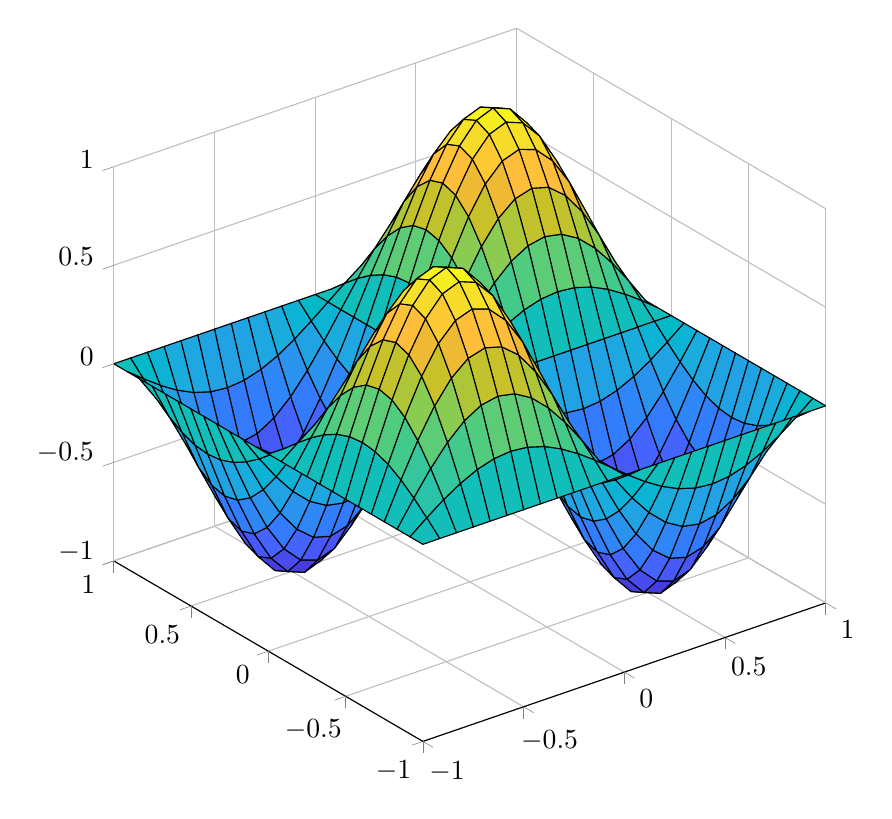
\begin{tikzpicture}

\begin{axis}[%
width=3.56in,
height=3.566in,
at={(0.597in,0.481in)},
scale only axis,
xmin=-1,
xmax=1,
tick align=outside,
ymin=-1,
ymax=1,
zmin=-1,
zmax=1,
view={-37.5}{30},
axis background/.style={fill=white},
axis x line*=bottom,
axis y line*=left,
axis z line*=left,
xmajorgrids,
ymajorgrids,
zmajorgrids,
legend style={at={(1.03,1)}, anchor=north west, legend cell align=left, align=left, draw=white!15!black}
]

\addplot3[%
surf,
shader=flat corner, draw=black, z buffer=sort, colormap={mymap}{[1pt] rgb(0pt)=(0.2422,0.1504,0.6603); rgb(1pt)=(0.25039,0.164995,0.707614); rgb(2pt)=(0.257771,0.181781,0.751138); rgb(3pt)=(0.264729,0.197757,0.795214); rgb(4pt)=(0.270648,0.214676,0.836371); rgb(5pt)=(0.275114,0.234238,0.870986); rgb(6pt)=(0.2783,0.255871,0.899071); rgb(7pt)=(0.280333,0.278233,0.9221); rgb(8pt)=(0.281338,0.300595,0.941376); rgb(9pt)=(0.281014,0.322757,0.957886); rgb(10pt)=(0.279467,0.344671,0.971676); rgb(11pt)=(0.275971,0.366681,0.982905); rgb(12pt)=(0.269914,0.3892,0.9906); rgb(13pt)=(0.260243,0.412329,0.995157); rgb(14pt)=(0.244033,0.435833,0.998833); rgb(15pt)=(0.220643,0.460257,0.997286); rgb(16pt)=(0.196333,0.484719,0.989152); rgb(17pt)=(0.183405,0.507371,0.979795); rgb(18pt)=(0.178643,0.528857,0.968157); rgb(19pt)=(0.176438,0.549905,0.952019); rgb(20pt)=(0.168743,0.570262,0.935871); rgb(21pt)=(0.154,0.5902,0.9218); rgb(22pt)=(0.146029,0.609119,0.907857); rgb(23pt)=(0.138024,0.627629,0.89729); rgb(24pt)=(0.124814,0.645929,0.888343); rgb(25pt)=(0.111252,0.6635,0.876314); rgb(26pt)=(0.0952095,0.679829,0.859781); rgb(27pt)=(0.0688714,0.694771,0.839357); rgb(28pt)=(0.0296667,0.708167,0.816333); rgb(29pt)=(0.00357143,0.720267,0.7917); rgb(30pt)=(0.00665714,0.731214,0.766014); rgb(31pt)=(0.0433286,0.741095,0.73941); rgb(32pt)=(0.0963952,0.75,0.712038); rgb(33pt)=(0.140771,0.7584,0.684157); rgb(34pt)=(0.1717,0.766962,0.655443); rgb(35pt)=(0.193767,0.775767,0.6251); rgb(36pt)=(0.216086,0.7843,0.5923); rgb(37pt)=(0.246957,0.791795,0.556743); rgb(38pt)=(0.290614,0.79729,0.518829); rgb(39pt)=(0.340643,0.8008,0.478857); rgb(40pt)=(0.3909,0.802871,0.435448); rgb(41pt)=(0.445629,0.802419,0.390919); rgb(42pt)=(0.5044,0.7993,0.348); rgb(43pt)=(0.561562,0.794233,0.304481); rgb(44pt)=(0.617395,0.787619,0.261238); rgb(45pt)=(0.671986,0.779271,0.2227); rgb(46pt)=(0.7242,0.769843,0.191029); rgb(47pt)=(0.773833,0.759805,0.16461); rgb(48pt)=(0.820314,0.749814,0.153529); rgb(49pt)=(0.863433,0.7406,0.159633); rgb(50pt)=(0.903543,0.733029,0.177414); rgb(51pt)=(0.939257,0.728786,0.209957); rgb(52pt)=(0.972757,0.729771,0.239443); rgb(53pt)=(0.995648,0.743371,0.237148); rgb(54pt)=(0.996986,0.765857,0.219943); rgb(55pt)=(0.995205,0.789252,0.202762); rgb(56pt)=(0.9892,0.813567,0.188533); rgb(57pt)=(0.978629,0.838629,0.176557); rgb(58pt)=(0.967648,0.8639,0.16429); rgb(59pt)=(0.96101,0.889019,0.153676); rgb(60pt)=(0.959671,0.913457,0.142257); rgb(61pt)=(0.962795,0.937338,0.12651); rgb(62pt)=(0.969114,0.960629,0.106362); rgb(63pt)=(0.9769,0.9839,0.0805)}, mesh/rows=25]
table[row sep=crcr, point meta=\thisrow{c}] {%
%
x	y	z	c\\
-1	-1	1.49975978266186e-32	1.49975978266186e-32\\
-0.916666666666667	-1	0	0\\
-0.833333333333333	-1	6.12323399573676e-17	6.12323399573676e-17\\
-0.75	-1	8.65956056235493e-17	8.65956056235493e-17\\
-0.666666666666667	-1	1.06057523872491e-16	1.06057523872491e-16\\
-0.583333333333333	-1	1.18291797137867e-16	1.18291797137867e-16\\
-0.5	-1	1.22464679914735e-16	1.22464679914735e-16\\
-0.416666666666667	-1	1.18291797137867e-16	1.18291797137867e-16\\
-0.333333333333333	-1	1.06057523872491e-16	1.06057523872491e-16\\
-0.25	-1	8.65956056235493e-17	8.65956056235493e-17\\
-0.166666666666667	-1	6.12323399573676e-17	6.12323399573676e-17\\
-0.0833333333333334	-1	3.16961915143177e-17	3.16961915143177e-17\\
0	-1	-0	-0\\
0.0833333333333333	-1	-3.16961915143176e-17	-3.16961915143176e-17\\
0.166666666666667	-1	-6.12323399573677e-17	-6.12323399573677e-17\\
0.25	-1	-8.65956056235493e-17	-8.65956056235493e-17\\
0.333333333333333	-1	-1.06057523872491e-16	-1.06057523872491e-16\\
0.416666666666667	-1	-1.18291797137867e-16	-1.18291797137867e-16\\
0.5	-1	-1.22464679914735e-16	-1.22464679914735e-16\\
0.583333333333333	-1	-1.18291797137867e-16	-1.18291797137867e-16\\
0.666666666666667	-1	-1.06057523872491e-16	-1.06057523872491e-16\\
0.75	-1	-8.65956056235493e-17	-8.65956056235493e-17\\
0.833333333333333	-1	-6.12323399573677e-17	-6.12323399573677e-17\\
0.916666666666667	-1	-3.16961915143176e-17	-3.16961915143176e-17\\
1	-1	-1.49975978266186e-32	-1.49975978266186e-32\\
-1	-0.916666666666667	3.16961915143177e-17	3.16961915143177e-17\\
-0.916666666666667	-0.916666666666667	0.0669872981077808	0.0669872981077808\\
-0.833333333333333	-0.916666666666667	0.12940952255126	0.12940952255126\\
-0.75	-0.916666666666667	0.18301270189222	0.18301270189222\\
-0.666666666666667	-0.916666666666667	0.224143868042014	0.224143868042014\\
-0.583333333333333	-0.916666666666667	0.25	0.25\\
-0.5	-0.916666666666667	0.258819045102521	0.258819045102521\\
-0.416666666666667	-0.916666666666667	0.25	0.25\\
-0.333333333333333	-0.916666666666667	0.224143868042014	0.224143868042014\\
-0.25	-0.916666666666667	0.183012701892219	0.183012701892219\\
-0.166666666666667	-0.916666666666667	0.12940952255126	0.12940952255126\\
-0.0833333333333334	-0.916666666666667	0.0669872981077808	0.0669872981077808\\
0	-0.916666666666667	-0	-0\\
0.0833333333333333	-0.916666666666667	-0.0669872981077807	-0.0669872981077807\\
0.166666666666667	-0.916666666666667	-0.129409522551261	-0.129409522551261\\
0.25	-0.916666666666667	-0.183012701892219	-0.183012701892219\\
0.333333333333333	-0.916666666666667	-0.224143868042014	-0.224143868042014\\
0.416666666666667	-0.916666666666667	-0.25	-0.25\\
0.5	-0.916666666666667	-0.258819045102521	-0.258819045102521\\
0.583333333333333	-0.916666666666667	-0.25	-0.25\\
0.666666666666667	-0.916666666666667	-0.224143868042014	-0.224143868042014\\
0.75	-0.916666666666667	-0.18301270189222	-0.18301270189222\\
0.833333333333333	-0.916666666666667	-0.129409522551261	-0.129409522551261\\
0.916666666666667	-0.916666666666667	-0.0669872981077807	-0.0669872981077807\\
1	-0.916666666666667	-3.16961915143177e-17	-3.16961915143177e-17\\
-1	-0.833333333333333	6.12323399573676e-17	6.12323399573676e-17\\
-0.916666666666667	-0.833333333333333	0.12940952255126	0.12940952255126\\
-0.833333333333333	-0.833333333333333	0.25	0.25\\
-0.75	-0.833333333333333	0.353553390593274	0.353553390593274\\
-0.666666666666667	-0.833333333333333	0.433012701892219	0.433012701892219\\
-0.583333333333333	-0.833333333333333	0.482962913144534	0.482962913144534\\
-0.5	-0.833333333333333	0.5	0.5\\
-0.416666666666667	-0.833333333333333	0.482962913144534	0.482962913144534\\
-0.333333333333333	-0.833333333333333	0.433012701892219	0.433012701892219\\
-0.25	-0.833333333333333	0.353553390593274	0.353553390593274\\
-0.166666666666667	-0.833333333333333	0.25	0.25\\
-0.0833333333333334	-0.833333333333333	0.12940952255126	0.12940952255126\\
0	-0.833333333333333	-0	-0\\
0.0833333333333333	-0.833333333333333	-0.12940952255126	-0.12940952255126\\
0.166666666666667	-0.833333333333333	-0.25	-0.25\\
0.25	-0.833333333333333	-0.353553390593274	-0.353553390593274\\
0.333333333333333	-0.833333333333333	-0.433012701892219	-0.433012701892219\\
0.416666666666667	-0.833333333333333	-0.482962913144534	-0.482962913144534\\
0.5	-0.833333333333333	-0.5	-0.5\\
0.583333333333333	-0.833333333333333	-0.482962913144534	-0.482962913144534\\
0.666666666666667	-0.833333333333333	-0.433012701892219	-0.433012701892219\\
0.75	-0.833333333333333	-0.353553390593274	-0.353553390593274\\
0.833333333333333	-0.833333333333333	-0.25	-0.25\\
0.916666666666667	-0.833333333333333	-0.12940952255126	-0.12940952255126\\
1	-0.833333333333333	-6.12323399573676e-17	-6.12323399573676e-17\\
-1	-0.75	8.65956056235493e-17	8.65956056235493e-17\\
-0.916666666666667	-0.75	0.18301270189222	0.18301270189222\\
-0.833333333333333	-0.75	0.353553390593274	0.353553390593274\\
-0.75	-0.75	0.5	0.5\\
-0.666666666666667	-0.75	0.612372435695795	0.612372435695795\\
-0.583333333333333	-0.75	0.68301270189222	0.68301270189222\\
-0.5	-0.75	0.707106781186548	0.707106781186548\\
-0.416666666666667	-0.75	0.683012701892219	0.683012701892219\\
-0.333333333333333	-0.75	0.612372435695795	0.612372435695795\\
-0.25	-0.75	0.5	0.5\\
-0.166666666666667	-0.75	0.353553390593274	0.353553390593274\\
-0.0833333333333334	-0.75	0.183012701892219	0.183012701892219\\
0	-0.75	-0	-0\\
0.0833333333333333	-0.75	-0.183012701892219	-0.183012701892219\\
0.166666666666667	-0.75	-0.353553390593274	-0.353553390593274\\
0.25	-0.75	-0.5	-0.5\\
0.333333333333333	-0.75	-0.612372435695794	-0.612372435695794\\
0.416666666666667	-0.75	-0.683012701892219	-0.683012701892219\\
0.5	-0.75	-0.707106781186548	-0.707106781186548\\
0.583333333333333	-0.75	-0.68301270189222	-0.68301270189222\\
0.666666666666667	-0.75	-0.612372435695795	-0.612372435695795\\
0.75	-0.75	-0.5	-0.5\\
0.833333333333333	-0.75	-0.353553390593274	-0.353553390593274\\
0.916666666666667	-0.75	-0.183012701892219	-0.183012701892219\\
1	-0.75	-8.65956056235493e-17	-8.65956056235493e-17\\
-1	-0.666666666666667	1.06057523872491e-16	1.06057523872491e-16\\
-0.916666666666667	-0.666666666666667	0.224143868042014	0.224143868042014\\
-0.833333333333333	-0.666666666666667	0.433012701892219	0.433012701892219\\
-0.75	-0.666666666666667	0.612372435695795	0.612372435695795\\
-0.666666666666667	-0.666666666666667	0.75	0.75\\
-0.583333333333333	-0.666666666666667	0.836516303737808	0.836516303737808\\
-0.5	-0.666666666666667	0.866025403784439	0.866025403784439\\
-0.416666666666667	-0.666666666666667	0.836516303737808	0.836516303737808\\
-0.333333333333333	-0.666666666666667	0.75	0.75\\
-0.25	-0.666666666666667	0.612372435695794	0.612372435695794\\
-0.166666666666667	-0.666666666666667	0.433012701892219	0.433012701892219\\
-0.0833333333333334	-0.666666666666667	0.224143868042013	0.224143868042013\\
0	-0.666666666666667	-0	-0\\
0.0833333333333333	-0.666666666666667	-0.224143868042013	-0.224143868042013\\
0.166666666666667	-0.666666666666667	-0.433012701892219	-0.433012701892219\\
0.25	-0.666666666666667	-0.612372435695794	-0.612372435695794\\
0.333333333333333	-0.666666666666667	-0.75	-0.75\\
0.416666666666667	-0.666666666666667	-0.836516303737808	-0.836516303737808\\
0.5	-0.666666666666667	-0.866025403784439	-0.866025403784439\\
0.583333333333333	-0.666666666666667	-0.836516303737808	-0.836516303737808\\
0.666666666666667	-0.666666666666667	-0.75	-0.75\\
0.75	-0.666666666666667	-0.612372435695795	-0.612372435695795\\
0.833333333333333	-0.666666666666667	-0.43301270189222	-0.43301270189222\\
0.916666666666667	-0.666666666666667	-0.224143868042013	-0.224143868042013\\
1	-0.666666666666667	-1.06057523872491e-16	-1.06057523872491e-16\\
-1	-0.583333333333333	1.18291797137867e-16	1.18291797137867e-16\\
-0.916666666666667	-0.583333333333333	0.25	0.25\\
-0.833333333333333	-0.583333333333333	0.482962913144534	0.482962913144534\\
-0.75	-0.583333333333333	0.68301270189222	0.68301270189222\\
-0.666666666666667	-0.583333333333333	0.836516303737808	0.836516303737808\\
-0.583333333333333	-0.583333333333333	0.93301270189222	0.93301270189222\\
-0.5	-0.583333333333333	0.965925826289068	0.965925826289068\\
-0.416666666666667	-0.583333333333333	0.933012701892219	0.933012701892219\\
-0.333333333333333	-0.583333333333333	0.836516303737808	0.836516303737808\\
-0.25	-0.583333333333333	0.683012701892219	0.683012701892219\\
-0.166666666666667	-0.583333333333333	0.482962913144534	0.482962913144534\\
-0.0833333333333334	-0.583333333333333	0.25	0.25\\
0	-0.583333333333333	-0	-0\\
0.0833333333333333	-0.583333333333333	-0.25	-0.25\\
0.166666666666667	-0.583333333333333	-0.482962913144534	-0.482962913144534\\
0.25	-0.583333333333333	-0.683012701892219	-0.683012701892219\\
0.333333333333333	-0.583333333333333	-0.836516303737808	-0.836516303737808\\
0.416666666666667	-0.583333333333333	-0.93301270189222	-0.93301270189222\\
0.5	-0.583333333333333	-0.965925826289068	-0.965925826289068\\
0.583333333333333	-0.583333333333333	-0.93301270189222	-0.93301270189222\\
0.666666666666667	-0.583333333333333	-0.836516303737808	-0.836516303737808\\
0.75	-0.583333333333333	-0.68301270189222	-0.68301270189222\\
0.833333333333333	-0.583333333333333	-0.482962913144535	-0.482962913144535\\
0.916666666666667	-0.583333333333333	-0.25	-0.25\\
1	-0.583333333333333	-1.18291797137867e-16	-1.18291797137867e-16\\
-1	-0.5	1.22464679914735e-16	1.22464679914735e-16\\
-0.916666666666667	-0.5	0.258819045102521	0.258819045102521\\
-0.833333333333333	-0.5	0.5	0.5\\
-0.75	-0.5	0.707106781186548	0.707106781186548\\
-0.666666666666667	-0.5	0.866025403784439	0.866025403784439\\
-0.583333333333333	-0.5	0.965925826289068	0.965925826289068\\
-0.5	-0.5	1	1\\
-0.416666666666667	-0.5	0.965925826289068	0.965925826289068\\
-0.333333333333333	-0.5	0.866025403784439	0.866025403784439\\
-0.25	-0.5	0.707106781186547	0.707106781186547\\
-0.166666666666667	-0.5	0.5	0.5\\
-0.0833333333333334	-0.5	0.258819045102521	0.258819045102521\\
0	-0.5	-0	-0\\
0.0833333333333333	-0.5	-0.258819045102521	-0.258819045102521\\
0.166666666666667	-0.5	-0.5	-0.5\\
0.25	-0.5	-0.707106781186547	-0.707106781186547\\
0.333333333333333	-0.5	-0.866025403784438	-0.866025403784438\\
0.416666666666667	-0.5	-0.965925826289068	-0.965925826289068\\
0.5	-0.5	-1	-1\\
0.583333333333333	-0.5	-0.965925826289068	-0.965925826289068\\
0.666666666666667	-0.5	-0.866025403784439	-0.866025403784439\\
0.75	-0.5	-0.707106781186548	-0.707106781186548\\
0.833333333333333	-0.5	-0.5	-0.5\\
0.916666666666667	-0.5	-0.258819045102521	-0.258819045102521\\
1	-0.5	-1.22464679914735e-16	-1.22464679914735e-16\\
-1	-0.416666666666667	1.18291797137867e-16	1.18291797137867e-16\\
-0.916666666666667	-0.416666666666667	0.25	0.25\\
-0.833333333333333	-0.416666666666667	0.482962913144534	0.482962913144534\\
-0.75	-0.416666666666667	0.683012701892219	0.683012701892219\\
-0.666666666666667	-0.416666666666667	0.836516303737808	0.836516303737808\\
-0.583333333333333	-0.416666666666667	0.933012701892219	0.933012701892219\\
-0.5	-0.416666666666667	0.965925826289068	0.965925826289068\\
-0.416666666666667	-0.416666666666667	0.933012701892219	0.933012701892219\\
-0.333333333333333	-0.416666666666667	0.836516303737808	0.836516303737808\\
-0.25	-0.416666666666667	0.683012701892219	0.683012701892219\\
-0.166666666666667	-0.416666666666667	0.482962913144534	0.482962913144534\\
-0.0833333333333334	-0.416666666666667	0.25	0.25\\
0	-0.416666666666667	-0	-0\\
0.0833333333333333	-0.416666666666667	-0.25	-0.25\\
0.166666666666667	-0.416666666666667	-0.482962913144534	-0.482962913144534\\
0.25	-0.416666666666667	-0.683012701892219	-0.683012701892219\\
0.333333333333333	-0.416666666666667	-0.836516303737808	-0.836516303737808\\
0.416666666666667	-0.416666666666667	-0.933012701892219	-0.933012701892219\\
0.5	-0.416666666666667	-0.965925826289068	-0.965925826289068\\
0.583333333333333	-0.416666666666667	-0.933012701892219	-0.933012701892219\\
0.666666666666667	-0.416666666666667	-0.836516303737808	-0.836516303737808\\
0.75	-0.416666666666667	-0.683012701892219	-0.683012701892219\\
0.833333333333333	-0.416666666666667	-0.482962913144534	-0.482962913144534\\
0.916666666666667	-0.416666666666667	-0.25	-0.25\\
1	-0.416666666666667	-1.18291797137867e-16	-1.18291797137867e-16\\
-1	-0.333333333333333	1.06057523872491e-16	1.06057523872491e-16\\
-0.916666666666667	-0.333333333333333	0.224143868042014	0.224143868042014\\
-0.833333333333333	-0.333333333333333	0.433012701892219	0.433012701892219\\
-0.75	-0.333333333333333	0.612372435695795	0.612372435695795\\
-0.666666666666667	-0.333333333333333	0.75	0.75\\
-0.583333333333333	-0.333333333333333	0.836516303737808	0.836516303737808\\
-0.5	-0.333333333333333	0.866025403784439	0.866025403784439\\
-0.416666666666667	-0.333333333333333	0.836516303737808	0.836516303737808\\
-0.333333333333333	-0.333333333333333	0.75	0.75\\
-0.25	-0.333333333333333	0.612372435695794	0.612372435695794\\
-0.166666666666667	-0.333333333333333	0.433012701892219	0.433012701892219\\
-0.0833333333333334	-0.333333333333333	0.224143868042013	0.224143868042013\\
0	-0.333333333333333	-0	-0\\
0.0833333333333333	-0.333333333333333	-0.224143868042013	-0.224143868042013\\
0.166666666666667	-0.333333333333333	-0.433012701892219	-0.433012701892219\\
0.25	-0.333333333333333	-0.612372435695794	-0.612372435695794\\
0.333333333333333	-0.333333333333333	-0.75	-0.75\\
0.416666666666667	-0.333333333333333	-0.836516303737808	-0.836516303737808\\
0.5	-0.333333333333333	-0.866025403784439	-0.866025403784439\\
0.583333333333333	-0.333333333333333	-0.836516303737808	-0.836516303737808\\
0.666666666666667	-0.333333333333333	-0.75	-0.75\\
0.75	-0.333333333333333	-0.612372435695795	-0.612372435695795\\
0.833333333333333	-0.333333333333333	-0.43301270189222	-0.43301270189222\\
0.916666666666667	-0.333333333333333	-0.224143868042013	-0.224143868042013\\
1	-0.333333333333333	-1.06057523872491e-16	-1.06057523872491e-16\\
-1	-0.25	8.65956056235493e-17	8.65956056235493e-17\\
-0.916666666666667	-0.25	0.183012701892219	0.183012701892219\\
-0.833333333333333	-0.25	0.353553390593274	0.353553390593274\\
-0.75	-0.25	0.5	0.5\\
-0.666666666666667	-0.25	0.612372435695794	0.612372435695794\\
-0.583333333333333	-0.25	0.683012701892219	0.683012701892219\\
-0.5	-0.25	0.707106781186547	0.707106781186547\\
-0.416666666666667	-0.25	0.683012701892219	0.683012701892219\\
-0.333333333333333	-0.25	0.612372435695794	0.612372435695794\\
-0.25	-0.25	0.5	0.5\\
-0.166666666666667	-0.25	0.353553390593274	0.353553390593274\\
-0.0833333333333334	-0.25	0.183012701892219	0.183012701892219\\
0	-0.25	-0	-0\\
0.0833333333333333	-0.25	-0.183012701892219	-0.183012701892219\\
0.166666666666667	-0.25	-0.353553390593274	-0.353553390593274\\
0.25	-0.25	-0.5	-0.5\\
0.333333333333333	-0.25	-0.612372435695794	-0.612372435695794\\
0.416666666666667	-0.25	-0.683012701892219	-0.683012701892219\\
0.5	-0.25	-0.707106781186547	-0.707106781186547\\
0.583333333333333	-0.25	-0.683012701892219	-0.683012701892219\\
0.666666666666667	-0.25	-0.612372435695794	-0.612372435695794\\
0.75	-0.25	-0.5	-0.5\\
0.833333333333333	-0.25	-0.353553390593274	-0.353553390593274\\
0.916666666666667	-0.25	-0.183012701892219	-0.183012701892219\\
1	-0.25	-8.65956056235493e-17	-8.65956056235493e-17\\
-1	-0.166666666666667	6.12323399573676e-17	6.12323399573676e-17\\
-0.916666666666667	-0.166666666666667	0.12940952255126	0.12940952255126\\
-0.833333333333333	-0.166666666666667	0.25	0.25\\
-0.75	-0.166666666666667	0.353553390593274	0.353553390593274\\
-0.666666666666667	-0.166666666666667	0.433012701892219	0.433012701892219\\
-0.583333333333333	-0.166666666666667	0.482962913144534	0.482962913144534\\
-0.5	-0.166666666666667	0.5	0.5\\
-0.416666666666667	-0.166666666666667	0.482962913144534	0.482962913144534\\
-0.333333333333333	-0.166666666666667	0.433012701892219	0.433012701892219\\
-0.25	-0.166666666666667	0.353553390593274	0.353553390593274\\
-0.166666666666667	-0.166666666666667	0.25	0.25\\
-0.0833333333333334	-0.166666666666667	0.12940952255126	0.12940952255126\\
0	-0.166666666666667	-0	-0\\
0.0833333333333333	-0.166666666666667	-0.12940952255126	-0.12940952255126\\
0.166666666666667	-0.166666666666667	-0.25	-0.25\\
0.25	-0.166666666666667	-0.353553390593274	-0.353553390593274\\
0.333333333333333	-0.166666666666667	-0.433012701892219	-0.433012701892219\\
0.416666666666667	-0.166666666666667	-0.482962913144534	-0.482962913144534\\
0.5	-0.166666666666667	-0.5	-0.5\\
0.583333333333333	-0.166666666666667	-0.482962913144534	-0.482962913144534\\
0.666666666666667	-0.166666666666667	-0.433012701892219	-0.433012701892219\\
0.75	-0.166666666666667	-0.353553390593274	-0.353553390593274\\
0.833333333333333	-0.166666666666667	-0.25	-0.25\\
0.916666666666667	-0.166666666666667	-0.12940952255126	-0.12940952255126\\
1	-0.166666666666667	-6.12323399573676e-17	-6.12323399573676e-17\\
-1	-0.0833333333333334	3.16961915143177e-17	3.16961915143177e-17\\
-0.916666666666667	-0.0833333333333334	0.0669872981077808	0.0669872981077808\\
-0.833333333333333	-0.0833333333333334	0.12940952255126	0.12940952255126\\
-0.75	-0.0833333333333334	0.183012701892219	0.183012701892219\\
-0.666666666666667	-0.0833333333333334	0.224143868042013	0.224143868042013\\
-0.583333333333333	-0.0833333333333334	0.25	0.25\\
-0.5	-0.0833333333333334	0.258819045102521	0.258819045102521\\
-0.416666666666667	-0.0833333333333334	0.25	0.25\\
-0.333333333333333	-0.0833333333333334	0.224143868042013	0.224143868042013\\
-0.25	-0.0833333333333334	0.183012701892219	0.183012701892219\\
-0.166666666666667	-0.0833333333333334	0.12940952255126	0.12940952255126\\
-0.0833333333333334	-0.0833333333333334	0.0669872981077807	0.0669872981077807\\
0	-0.0833333333333334	-0	-0\\
0.0833333333333333	-0.0833333333333334	-0.0669872981077806	-0.0669872981077806\\
0.166666666666667	-0.0833333333333334	-0.12940952255126	-0.12940952255126\\
0.25	-0.0833333333333334	-0.183012701892219	-0.183012701892219\\
0.333333333333333	-0.0833333333333334	-0.224143868042013	-0.224143868042013\\
0.416666666666667	-0.0833333333333334	-0.25	-0.25\\
0.5	-0.0833333333333334	-0.258819045102521	-0.258819045102521\\
0.583333333333333	-0.0833333333333334	-0.25	-0.25\\
0.666666666666667	-0.0833333333333334	-0.224143868042013	-0.224143868042013\\
0.75	-0.0833333333333334	-0.183012701892219	-0.183012701892219\\
0.833333333333333	-0.0833333333333334	-0.129409522551261	-0.129409522551261\\
0.916666666666667	-0.0833333333333334	-0.0669872981077806	-0.0669872981077806\\
1	-0.0833333333333334	-3.16961915143177e-17	-3.16961915143177e-17\\
-1	0	-0	-0\\
-0.916666666666667	0	-0	-0\\
-0.833333333333333	0	-0	-0\\
-0.75	0	-0	-0\\
-0.666666666666667	0	-0	-0\\
-0.583333333333333	0	-0	-0\\
-0.5	0	-0	-0\\
-0.416666666666667	0	-0	-0\\
-0.333333333333333	0	-0	-0\\
-0.25	0	-0	-0\\
-0.166666666666667	0	-0	-0\\
-0.0833333333333334	0	-0	-0\\
0	0	0	0\\
0.0833333333333333	0	0	0\\
0.166666666666667	0	0	0\\
0.25	0	0	0\\
0.333333333333333	0	0	0\\
0.416666666666667	0	0	0\\
0.5	0	0	0\\
0.583333333333333	0	0	0\\
0.666666666666667	0	0	0\\
0.75	0	0	0\\
0.833333333333333	0	0	0\\
0.916666666666667	0	0	0\\
1	0	0	0\\
-1	0.0833333333333333	-3.16961915143176e-17	-3.16961915143176e-17\\
-0.916666666666667	0.0833333333333333	-0.0669872981077807	-0.0669872981077807\\
-0.833333333333333	0.0833333333333333	-0.12940952255126	-0.12940952255126\\
-0.75	0.0833333333333333	-0.183012701892219	-0.183012701892219\\
-0.666666666666667	0.0833333333333333	-0.224143868042013	-0.224143868042013\\
-0.583333333333333	0.0833333333333333	-0.25	-0.25\\
-0.5	0.0833333333333333	-0.258819045102521	-0.258819045102521\\
-0.416666666666667	0.0833333333333333	-0.25	-0.25\\
-0.333333333333333	0.0833333333333333	-0.224143868042013	-0.224143868042013\\
-0.25	0.0833333333333333	-0.183012701892219	-0.183012701892219\\
-0.166666666666667	0.0833333333333333	-0.12940952255126	-0.12940952255126\\
-0.0833333333333334	0.0833333333333333	-0.0669872981077806	-0.0669872981077806\\
0	0.0833333333333333	0	0\\
0.0833333333333333	0.0833333333333333	0.0669872981077805	0.0669872981077805\\
0.166666666666667	0.0833333333333333	0.12940952255126	0.12940952255126\\
0.25	0.0833333333333333	0.183012701892219	0.183012701892219\\
0.333333333333333	0.0833333333333333	0.224143868042013	0.224143868042013\\
0.416666666666667	0.0833333333333333	0.25	0.25\\
0.5	0.0833333333333333	0.258819045102521	0.258819045102521\\
0.583333333333333	0.0833333333333333	0.25	0.25\\
0.666666666666667	0.0833333333333333	0.224143868042013	0.224143868042013\\
0.75	0.0833333333333333	0.183012701892219	0.183012701892219\\
0.833333333333333	0.0833333333333333	0.12940952255126	0.12940952255126\\
0.916666666666667	0.0833333333333333	0.0669872981077806	0.0669872981077806\\
1	0.0833333333333333	3.16961915143176e-17	3.16961915143176e-17\\
-1	0.166666666666667	-6.12323399573677e-17	-6.12323399573677e-17\\
-0.916666666666667	0.166666666666667	-0.129409522551261	-0.129409522551261\\
-0.833333333333333	0.166666666666667	-0.25	-0.25\\
-0.75	0.166666666666667	-0.353553390593274	-0.353553390593274\\
-0.666666666666667	0.166666666666667	-0.433012701892219	-0.433012701892219\\
-0.583333333333333	0.166666666666667	-0.482962913144534	-0.482962913144534\\
-0.5	0.166666666666667	-0.5	-0.5\\
-0.416666666666667	0.166666666666667	-0.482962913144534	-0.482962913144534\\
-0.333333333333333	0.166666666666667	-0.433012701892219	-0.433012701892219\\
-0.25	0.166666666666667	-0.353553390593274	-0.353553390593274\\
-0.166666666666667	0.166666666666667	-0.25	-0.25\\
-0.0833333333333334	0.166666666666667	-0.12940952255126	-0.12940952255126\\
0	0.166666666666667	0	0\\
0.0833333333333333	0.166666666666667	0.12940952255126	0.12940952255126\\
0.166666666666667	0.166666666666667	0.25	0.25\\
0.25	0.166666666666667	0.353553390593274	0.353553390593274\\
0.333333333333333	0.166666666666667	0.433012701892219	0.433012701892219\\
0.416666666666667	0.166666666666667	0.482962913144534	0.482962913144534\\
0.5	0.166666666666667	0.5	0.5\\
0.583333333333333	0.166666666666667	0.482962913144534	0.482962913144534\\
0.666666666666667	0.166666666666667	0.433012701892219	0.433012701892219\\
0.75	0.166666666666667	0.353553390593274	0.353553390593274\\
0.833333333333333	0.166666666666667	0.25	0.25\\
0.916666666666667	0.166666666666667	0.12940952255126	0.12940952255126\\
1	0.166666666666667	6.12323399573677e-17	6.12323399573677e-17\\
-1	0.25	-8.65956056235493e-17	-8.65956056235493e-17\\
-0.916666666666667	0.25	-0.183012701892219	-0.183012701892219\\
-0.833333333333333	0.25	-0.353553390593274	-0.353553390593274\\
-0.75	0.25	-0.5	-0.5\\
-0.666666666666667	0.25	-0.612372435695794	-0.612372435695794\\
-0.583333333333333	0.25	-0.683012701892219	-0.683012701892219\\
-0.5	0.25	-0.707106781186547	-0.707106781186547\\
-0.416666666666667	0.25	-0.683012701892219	-0.683012701892219\\
-0.333333333333333	0.25	-0.612372435695794	-0.612372435695794\\
-0.25	0.25	-0.5	-0.5\\
-0.166666666666667	0.25	-0.353553390593274	-0.353553390593274\\
-0.0833333333333334	0.25	-0.183012701892219	-0.183012701892219\\
0	0.25	0	0\\
0.0833333333333333	0.25	0.183012701892219	0.183012701892219\\
0.166666666666667	0.25	0.353553390593274	0.353553390593274\\
0.25	0.25	0.5	0.5\\
0.333333333333333	0.25	0.612372435695794	0.612372435695794\\
0.416666666666667	0.25	0.683012701892219	0.683012701892219\\
0.5	0.25	0.707106781186547	0.707106781186547\\
0.583333333333333	0.25	0.683012701892219	0.683012701892219\\
0.666666666666667	0.25	0.612372435695794	0.612372435695794\\
0.75	0.25	0.5	0.5\\
0.833333333333333	0.25	0.353553390593274	0.353553390593274\\
0.916666666666667	0.25	0.183012701892219	0.183012701892219\\
1	0.25	8.65956056235493e-17	8.65956056235493e-17\\
-1	0.333333333333333	-1.06057523872491e-16	-1.06057523872491e-16\\
-0.916666666666667	0.333333333333333	-0.224143868042014	-0.224143868042014\\
-0.833333333333333	0.333333333333333	-0.433012701892219	-0.433012701892219\\
-0.75	0.333333333333333	-0.612372435695794	-0.612372435695794\\
-0.666666666666667	0.333333333333333	-0.75	-0.75\\
-0.583333333333333	0.333333333333333	-0.836516303737808	-0.836516303737808\\
-0.5	0.333333333333333	-0.866025403784438	-0.866025403784438\\
-0.416666666666667	0.333333333333333	-0.836516303737808	-0.836516303737808\\
-0.333333333333333	0.333333333333333	-0.75	-0.75\\
-0.25	0.333333333333333	-0.612372435695794	-0.612372435695794\\
-0.166666666666667	0.333333333333333	-0.433012701892219	-0.433012701892219\\
-0.0833333333333334	0.333333333333333	-0.224143868042013	-0.224143868042013\\
0	0.333333333333333	0	0\\
0.0833333333333333	0.333333333333333	0.224143868042013	0.224143868042013\\
0.166666666666667	0.333333333333333	0.433012701892219	0.433012701892219\\
0.25	0.333333333333333	0.612372435695794	0.612372435695794\\
0.333333333333333	0.333333333333333	0.75	0.75\\
0.416666666666667	0.333333333333333	0.836516303737808	0.836516303737808\\
0.5	0.333333333333333	0.866025403784438	0.866025403784438\\
0.583333333333333	0.333333333333333	0.836516303737808	0.836516303737808\\
0.666666666666667	0.333333333333333	0.75	0.75\\
0.75	0.333333333333333	0.612372435695794	0.612372435695794\\
0.833333333333333	0.333333333333333	0.43301270189222	0.43301270189222\\
0.916666666666667	0.333333333333333	0.224143868042013	0.224143868042013\\
1	0.333333333333333	1.06057523872491e-16	1.06057523872491e-16\\
-1	0.416666666666667	-1.18291797137867e-16	-1.18291797137867e-16\\
-0.916666666666667	0.416666666666667	-0.25	-0.25\\
-0.833333333333333	0.416666666666667	-0.482962913144534	-0.482962913144534\\
-0.75	0.416666666666667	-0.683012701892219	-0.683012701892219\\
-0.666666666666667	0.416666666666667	-0.836516303737808	-0.836516303737808\\
-0.583333333333333	0.416666666666667	-0.93301270189222	-0.93301270189222\\
-0.5	0.416666666666667	-0.965925826289068	-0.965925826289068\\
-0.416666666666667	0.416666666666667	-0.933012701892219	-0.933012701892219\\
-0.333333333333333	0.416666666666667	-0.836516303737808	-0.836516303737808\\
-0.25	0.416666666666667	-0.683012701892219	-0.683012701892219\\
-0.166666666666667	0.416666666666667	-0.482962913144534	-0.482962913144534\\
-0.0833333333333334	0.416666666666667	-0.25	-0.25\\
0	0.416666666666667	0	0\\
0.0833333333333333	0.416666666666667	0.25	0.25\\
0.166666666666667	0.416666666666667	0.482962913144534	0.482962913144534\\
0.25	0.416666666666667	0.683012701892219	0.683012701892219\\
0.333333333333333	0.416666666666667	0.836516303737808	0.836516303737808\\
0.416666666666667	0.416666666666667	0.933012701892219	0.933012701892219\\
0.5	0.416666666666667	0.965925826289068	0.965925826289068\\
0.583333333333333	0.416666666666667	0.93301270189222	0.93301270189222\\
0.666666666666667	0.416666666666667	0.836516303737808	0.836516303737808\\
0.75	0.416666666666667	0.683012701892219	0.683012701892219\\
0.833333333333333	0.416666666666667	0.482962913144534	0.482962913144534\\
0.916666666666667	0.416666666666667	0.25	0.25\\
1	0.416666666666667	1.18291797137867e-16	1.18291797137867e-16\\
-1	0.5	-1.22464679914735e-16	-1.22464679914735e-16\\
-0.916666666666667	0.5	-0.258819045102521	-0.258819045102521\\
-0.833333333333333	0.5	-0.5	-0.5\\
-0.75	0.5	-0.707106781186548	-0.707106781186548\\
-0.666666666666667	0.5	-0.866025403784439	-0.866025403784439\\
-0.583333333333333	0.5	-0.965925826289068	-0.965925826289068\\
-0.5	0.5	-1	-1\\
-0.416666666666667	0.5	-0.965925826289068	-0.965925826289068\\
-0.333333333333333	0.5	-0.866025403784439	-0.866025403784439\\
-0.25	0.5	-0.707106781186547	-0.707106781186547\\
-0.166666666666667	0.5	-0.5	-0.5\\
-0.0833333333333334	0.5	-0.258819045102521	-0.258819045102521\\
0	0.5	0	0\\
0.0833333333333333	0.5	0.258819045102521	0.258819045102521\\
0.166666666666667	0.5	0.5	0.5\\
0.25	0.5	0.707106781186547	0.707106781186547\\
0.333333333333333	0.5	0.866025403784438	0.866025403784438\\
0.416666666666667	0.5	0.965925826289068	0.965925826289068\\
0.5	0.5	1	1\\
0.583333333333333	0.5	0.965925826289068	0.965925826289068\\
0.666666666666667	0.5	0.866025403784439	0.866025403784439\\
0.75	0.5	0.707106781186548	0.707106781186548\\
0.833333333333333	0.5	0.5	0.5\\
0.916666666666667	0.5	0.258819045102521	0.258819045102521\\
1	0.5	1.22464679914735e-16	1.22464679914735e-16\\
-1	0.583333333333333	-1.18291797137867e-16	-1.18291797137867e-16\\
-0.916666666666667	0.583333333333333	-0.25	-0.25\\
-0.833333333333333	0.583333333333333	-0.482962913144534	-0.482962913144534\\
-0.75	0.583333333333333	-0.68301270189222	-0.68301270189222\\
-0.666666666666667	0.583333333333333	-0.836516303737808	-0.836516303737808\\
-0.583333333333333	0.583333333333333	-0.93301270189222	-0.93301270189222\\
-0.5	0.583333333333333	-0.965925826289068	-0.965925826289068\\
-0.416666666666667	0.583333333333333	-0.933012701892219	-0.933012701892219\\
-0.333333333333333	0.583333333333333	-0.836516303737808	-0.836516303737808\\
-0.25	0.583333333333333	-0.683012701892219	-0.683012701892219\\
-0.166666666666667	0.583333333333333	-0.482962913144534	-0.482962913144534\\
-0.0833333333333334	0.583333333333333	-0.25	-0.25\\
0	0.583333333333333	0	0\\
0.0833333333333333	0.583333333333333	0.25	0.25\\
0.166666666666667	0.583333333333333	0.482962913144534	0.482962913144534\\
0.25	0.583333333333333	0.683012701892219	0.683012701892219\\
0.333333333333333	0.583333333333333	0.836516303737808	0.836516303737808\\
0.416666666666667	0.583333333333333	0.93301270189222	0.93301270189222\\
0.5	0.583333333333333	0.965925826289068	0.965925826289068\\
0.583333333333333	0.583333333333333	0.93301270189222	0.93301270189222\\
0.666666666666667	0.583333333333333	0.836516303737808	0.836516303737808\\
0.75	0.583333333333333	0.68301270189222	0.68301270189222\\
0.833333333333333	0.583333333333333	0.482962913144535	0.482962913144535\\
0.916666666666667	0.583333333333333	0.25	0.25\\
1	0.583333333333333	1.18291797137867e-16	1.18291797137867e-16\\
-1	0.666666666666667	-1.06057523872491e-16	-1.06057523872491e-16\\
-0.916666666666667	0.666666666666667	-0.224143868042014	-0.224143868042014\\
-0.833333333333333	0.666666666666667	-0.433012701892219	-0.433012701892219\\
-0.75	0.666666666666667	-0.612372435695795	-0.612372435695795\\
-0.666666666666667	0.666666666666667	-0.75	-0.75\\
-0.583333333333333	0.666666666666667	-0.836516303737808	-0.836516303737808\\
-0.5	0.666666666666667	-0.866025403784439	-0.866025403784439\\
-0.416666666666667	0.666666666666667	-0.836516303737808	-0.836516303737808\\
-0.333333333333333	0.666666666666667	-0.75	-0.75\\
-0.25	0.666666666666667	-0.612372435695794	-0.612372435695794\\
-0.166666666666667	0.666666666666667	-0.433012701892219	-0.433012701892219\\
-0.0833333333333334	0.666666666666667	-0.224143868042013	-0.224143868042013\\
0	0.666666666666667	0	0\\
0.0833333333333333	0.666666666666667	0.224143868042013	0.224143868042013\\
0.166666666666667	0.666666666666667	0.433012701892219	0.433012701892219\\
0.25	0.666666666666667	0.612372435695794	0.612372435695794\\
0.333333333333333	0.666666666666667	0.75	0.75\\
0.416666666666667	0.666666666666667	0.836516303737808	0.836516303737808\\
0.5	0.666666666666667	0.866025403784439	0.866025403784439\\
0.583333333333333	0.666666666666667	0.836516303737808	0.836516303737808\\
0.666666666666667	0.666666666666667	0.75	0.75\\
0.75	0.666666666666667	0.612372435695795	0.612372435695795\\
0.833333333333333	0.666666666666667	0.43301270189222	0.43301270189222\\
0.916666666666667	0.666666666666667	0.224143868042013	0.224143868042013\\
1	0.666666666666667	1.06057523872491e-16	1.06057523872491e-16\\
-1	0.75	-8.65956056235493e-17	-8.65956056235493e-17\\
-0.916666666666667	0.75	-0.18301270189222	-0.18301270189222\\
-0.833333333333333	0.75	-0.353553390593274	-0.353553390593274\\
-0.75	0.75	-0.5	-0.5\\
-0.666666666666667	0.75	-0.612372435695795	-0.612372435695795\\
-0.583333333333333	0.75	-0.68301270189222	-0.68301270189222\\
-0.5	0.75	-0.707106781186548	-0.707106781186548\\
-0.416666666666667	0.75	-0.683012701892219	-0.683012701892219\\
-0.333333333333333	0.75	-0.612372435695795	-0.612372435695795\\
-0.25	0.75	-0.5	-0.5\\
-0.166666666666667	0.75	-0.353553390593274	-0.353553390593274\\
-0.0833333333333334	0.75	-0.183012701892219	-0.183012701892219\\
0	0.75	0	0\\
0.0833333333333333	0.75	0.183012701892219	0.183012701892219\\
0.166666666666667	0.75	0.353553390593274	0.353553390593274\\
0.25	0.75	0.5	0.5\\
0.333333333333333	0.75	0.612372435695794	0.612372435695794\\
0.416666666666667	0.75	0.683012701892219	0.683012701892219\\
0.5	0.75	0.707106781186548	0.707106781186548\\
0.583333333333333	0.75	0.68301270189222	0.68301270189222\\
0.666666666666667	0.75	0.612372435695795	0.612372435695795\\
0.75	0.75	0.5	0.5\\
0.833333333333333	0.75	0.353553390593274	0.353553390593274\\
0.916666666666667	0.75	0.183012701892219	0.183012701892219\\
1	0.75	8.65956056235493e-17	8.65956056235493e-17\\
-1	0.833333333333333	0	0\\
-0.916666666666667	0.833333333333333	-0.129409522551261	-0.129409522551261\\
-0.833333333333333	0.833333333333333	-0.25	-0.25\\
-0.75	0.833333333333333	-0.353553390593274	-0.353553390593274\\
-0.666666666666667	0.833333333333333	-0.43301270189222	-0.43301270189222\\
-0.583333333333333	0.833333333333333	-0.482962913144535	-0.482962913144535\\
-0.5	0.833333333333333	-0.5	-0.5\\
-0.416666666666667	0.833333333333333	-0.482962913144534	-0.482962913144534\\
-0.333333333333333	0.833333333333333	-0.43301270189222	-0.43301270189222\\
-0.25	0.833333333333333	-0.353553390593274	-0.353553390593274\\
-0.166666666666667	0.833333333333333	-0.25	-0.25\\
-0.0833333333333334	0.833333333333333	-0.129409522551261	-0.129409522551261\\
0	0.833333333333333	0	0\\
0.0833333333333333	0.833333333333333	0.12940952255126	0.12940952255126\\
0.166666666666667	0.833333333333333	0.25	0.25\\
0.25	0.833333333333333	0.353553390593274	0.353553390593274\\
0.333333333333333	0.833333333333333	0.43301270189222	0.43301270189222\\
0.416666666666667	0.833333333333333	0.482962913144534	0.482962913144534\\
0.5	0.833333333333333	0.5	0.5\\
0.583333333333333	0.833333333333333	0.482962913144535	0.482962913144535\\
0.666666666666667	0.833333333333333	0.43301270189222	0.43301270189222\\
0.75	0.833333333333333	0.353553390593274	0.353553390593274\\
0.833333333333333	0.833333333333333	0.25	0.25\\
0.916666666666667	0.833333333333333	0.12940952255126	0.12940952255126\\
1	0.833333333333333	0	0\\
-1	0.916666666666667	-3.16961915143176e-17	-3.16961915143176e-17\\
-0.916666666666667	0.916666666666667	-0.0669872981077807	-0.0669872981077807\\
-0.833333333333333	0.916666666666667	-0.12940952255126	-0.12940952255126\\
-0.75	0.916666666666667	-0.183012701892219	-0.183012701892219\\
-0.666666666666667	0.916666666666667	-0.224143868042013	-0.224143868042013\\
-0.583333333333333	0.916666666666667	-0.25	-0.25\\
-0.5	0.916666666666667	-0.258819045102521	-0.258819045102521\\
-0.416666666666667	0.916666666666667	-0.25	-0.25\\
-0.333333333333333	0.916666666666667	-0.224143868042013	-0.224143868042013\\
-0.25	0.916666666666667	-0.183012701892219	-0.183012701892219\\
-0.166666666666667	0.916666666666667	-0.12940952255126	-0.12940952255126\\
-0.0833333333333334	0.916666666666667	-0.0669872981077806	-0.0669872981077806\\
0	0.916666666666667	0	0\\
0.0833333333333333	0.916666666666667	0.0669872981077806	0.0669872981077806\\
0.166666666666667	0.916666666666667	0.12940952255126	0.12940952255126\\
0.25	0.916666666666667	0.183012701892219	0.183012701892219\\
0.333333333333333	0.916666666666667	0.224143868042013	0.224143868042013\\
0.416666666666667	0.916666666666667	0.25	0.25\\
0.5	0.916666666666667	0.258819045102521	0.258819045102521\\
0.583333333333333	0.916666666666667	0.25	0.25\\
0.666666666666667	0.916666666666667	0.224143868042013	0.224143868042013\\
0.75	0.916666666666667	0.183012701892219	0.183012701892219\\
0.833333333333333	0.916666666666667	0.12940952255126	0.12940952255126\\
0.916666666666667	0.916666666666667	0.0669872981077806	0.0669872981077806\\
1	0.916666666666667	3.16961915143176e-17	3.16961915143176e-17\\
-1	1	-1.49975978266186e-32	-1.49975978266186e-32\\
-0.916666666666667	1	0	0\\
-0.833333333333333	1	-6.12323399573676e-17	-6.12323399573676e-17\\
-0.75	1	-8.65956056235493e-17	-8.65956056235493e-17\\
-0.666666666666667	1	-1.06057523872491e-16	-1.06057523872491e-16\\
-0.583333333333333	1	-1.18291797137867e-16	-1.18291797137867e-16\\
-0.5	1	-1.22464679914735e-16	-1.22464679914735e-16\\
-0.416666666666667	1	-1.18291797137867e-16	-1.18291797137867e-16\\
-0.333333333333333	1	-1.06057523872491e-16	-1.06057523872491e-16\\
-0.25	1	-8.65956056235493e-17	-8.65956056235493e-17\\
-0.166666666666667	1	-6.12323399573676e-17	-6.12323399573676e-17\\
-0.0833333333333334	1	-3.16961915143177e-17	-3.16961915143177e-17\\
0	1	0	0\\
0.0833333333333333	1	3.16961915143176e-17	3.16961915143176e-17\\
0.166666666666667	1	6.12323399573677e-17	6.12323399573677e-17\\
0.25	1	8.65956056235493e-17	8.65956056235493e-17\\
0.333333333333333	1	1.06057523872491e-16	1.06057523872491e-16\\
0.416666666666667	1	1.18291797137867e-16	1.18291797137867e-16\\
0.5	1	1.22464679914735e-16	1.22464679914735e-16\\
0.583333333333333	1	1.18291797137867e-16	1.18291797137867e-16\\
0.666666666666667	1	1.06057523872491e-16	1.06057523872491e-16\\
0.75	1	8.65956056235493e-17	8.65956056235493e-17\\
0.833333333333333	1	6.12323399573677e-17	6.12323399573677e-17\\
0.916666666666667	1	3.16961915143176e-17	3.16961915143176e-17\\
1	1	1.49975978266186e-32	1.49975978266186e-32\\
};
%\addlegendentry{data1}

\end{axis}
\end{tikzpicture}%
}
\caption{Lösung der \acs{PDE}}
\label{fig:plot}
\end{figure}

Diese werden wir mithilfe der Kernkollokation numerisch lösen. Dafür wählen wir den Gauß Kern aus Beispiel \ref{ex:Kern}. Aufgrund der fehlenden Praxisrelevanz werden wir die erste in Kapitel \ref{cha:Implementierung} vorgestellte Methode zur Fehlerberechnung in jeder Iteration nicht betrachten, sondern nur die in der Ableitung.

\section{Fehler}
\subsection{Absoluter Fehler}

Als Maß des Fehlers unserer numerischen Lösung wollen wir den maximalen absoluten Fehler zur analytischen Lösung berechnen, also
\begin{align*}
\text{error} = \max_{x \in \Omega} |u(x) - s_u (x)|,
\end{align*}
wobei $s_u$ die numerische Lösung bezeichnet.

Wir werden die drei in Kapitel \ref{cha:Implementierung} vorgestellten Methoden zur Kollokationspunktwahl testen und miteinander vergleichen. 
\subsubsection{Kollokationspunkte als Gitter}
Wir werden die Kollokationspunkte, so wie die Testpunkte, zunächst, wie in Abbildung \ref{fig:Kollok} gezeigt, in einem Gitter anordnen.
\begin{figure}[ht]
\centering
\resizebox {.8\columnwidth} {!} {
% This file was created by matlab2tikz.
%
%The latest updates can be retrieved from
%  http://www.mathworks.com/matlabcentral/fileexchange/22022-matlab2tikz-matlab2tikz
%where you can also make suggestions and rate matlab2tikz.
%
\definecolor{mycolor1}{rgb}{0.00000,0.44700,0.74100}%
%
\begin{tikzpicture}

\begin{axis}[%
width=4.in,
height=4.in,
at={(0.983in,0.681in)},
scale only axis,
xmin=-1,
xmax=1,
ymin=-1,
ymax=1,
axis background/.style={fill=white},
axis x line*=bottom,
axis y line*=left,
legend style={legend cell align=left, align=left, draw=white!15!black}
]
\addplot [color=red, draw=none, mark=+, mark options={solid, red}]
  table[row sep=crcr]{%
-0.777777777777778	-0.777777777777778\\
-0.555555555555556	-0.777777777777778\\
-0.333333333333333	-0.777777777777778\\
-0.111111111111111	-0.777777777777778\\
0.111111111111111	-0.777777777777778\\
0.333333333333333	-0.777777777777778\\
0.555555555555556	-0.777777777777778\\
0.777777777777778	-0.777777777777778\\
-0.777777777777778	-0.555555555555556\\
-0.555555555555556	-0.555555555555556\\
-0.333333333333333	-0.555555555555556\\
-0.111111111111111	-0.555555555555556\\
0.111111111111111	-0.555555555555556\\
0.333333333333333	-0.555555555555556\\
0.555555555555556	-0.555555555555556\\
0.777777777777778	-0.555555555555556\\
-0.777777777777778	-0.333333333333333\\
-0.555555555555556	-0.333333333333333\\
-0.333333333333333	-0.333333333333333\\
-0.111111111111111	-0.333333333333333\\
0.111111111111111	-0.333333333333333\\
0.333333333333333	-0.333333333333333\\
0.555555555555556	-0.333333333333333\\
0.777777777777778	-0.333333333333333\\
-0.777777777777778	-0.111111111111111\\
-0.555555555555556	-0.111111111111111\\
-0.333333333333333	-0.111111111111111\\
-0.111111111111111	-0.111111111111111\\
0.111111111111111	-0.111111111111111\\
0.333333333333333	-0.111111111111111\\
0.555555555555556	-0.111111111111111\\
0.777777777777778	-0.111111111111111\\
-0.777777777777778	0.111111111111111\\
-0.555555555555556	0.111111111111111\\
-0.333333333333333	0.111111111111111\\
-0.111111111111111	0.111111111111111\\
0.111111111111111	0.111111111111111\\
0.333333333333333	0.111111111111111\\
0.555555555555556	0.111111111111111\\
0.777777777777778	0.111111111111111\\
-0.777777777777778	0.333333333333333\\
-0.555555555555556	0.333333333333333\\
-0.333333333333333	0.333333333333333\\
-0.111111111111111	0.333333333333333\\
0.111111111111111	0.333333333333333\\
0.333333333333333	0.333333333333333\\
0.555555555555556	0.333333333333333\\
0.777777777777778	0.333333333333333\\
-0.777777777777778	0.555555555555556\\
-0.555555555555556	0.555555555555556\\
-0.333333333333333	0.555555555555556\\
-0.111111111111111	0.555555555555556\\
0.111111111111111	0.555555555555556\\
0.333333333333333	0.555555555555556\\
0.555555555555556	0.555555555555556\\
0.777777777777778	0.555555555555556\\
-0.777777777777778	0.777777777777778\\
-0.555555555555556	0.777777777777778\\
-0.333333333333333	0.777777777777778\\
-0.111111111111111	0.777777777777778\\
0.111111111111111	0.777777777777778\\
0.333333333333333	0.777777777777778\\
0.555555555555556	0.777777777777778\\
0.777777777777778	0.777777777777778\\
};
\addlegendentry{Kollokationspunkte}

\addplot [color=blue, draw=none, mark=asterisk, mark options={solid, blue}]
  table[row sep=crcr]{%
-0.5	-0.5\\
0	-0.5\\
0.5	-0.5\\
-0.5	0\\
0	0\\
0.5	0\\
-0.5	0.5\\
0	0.5\\
0.5	0.5\\
};
\addlegendentry{Validationspunkte}

\addplot [color=mycolor1, forget plot]
  table[row sep=crcr]{%
-1	-1\\
-1	1\\
1	1\\
1	-1\\
-1	-1\\
};
\end{axis}
\end{tikzpicture}%
}
\caption{Kollokationspunkte}
\label{fig:Kollok}
\end{figure}

Damit können wir uns anschauen, wie sich der Fehler bei Verfeinerung des Gitters verhält. Dieser ist in Abbildung \ref{fig:error} für die vier verschiedenen Verfahren dargestellt. 
\begin{figure}[ht]
\centering
\resizebox {\columnwidth} {!} {
\input{plots/error-grid.tex}
}
\caption{Fehler bei Kollokationspunkten auf Gitter}
\label{fig:error}
\end{figure}
%\begin{table}[H]
%\centering
%\begin{tabular}{c|c|c|c|c}
%%\hline 
% & $n = 9$ & $n = 100$ & $n = 1024$ & $n = 6084$ \\ 
%\hline 
%Standard N-Sym & \num{0.99974} & \num{2.18205e-04} & \num{2.61592e-06} & \num{9.07630e-06} \\ 
%%\hline 
%Standard Sym & \num{0.99974} & \num{2.48216e-05} & \num{1.08639e-07} & \num{1.31851e-07} \\ 
%%\hline 
%Gewichtet N-Sym & \num{0.37643} & \num{8.20819e-03} & \num{1.87889e-03} & \num{3.09914e-04} \\ 
%%\hline 
%Gewichtet Sym & \num{0.27994} & \num{6.40403e-03} & \num{1.04064e-03} & • \\ 
%%\hline 
%\end{tabular} 
%\caption{Vergleich der Verfahren}
%\label{tab:Vergleich Fehler}
%\end{table}

Wir stellen als erstes fest, dass alle Verfahren vernünftige Ergebnisse liefern und gegen die analytische Lösung konvergieren. Unsere theoretische Herleitung war demnach also sinnvoll. 

Wir erkennen, dass alle Verfahren sehr schnell gute Ergebnisse liefern. Die beiden Standardverfahren liefern bereits mit nahezu $200$ Kollokationspunkten ihre besten Ergebnisse in der Größenordnung von $10^{-6}$ für das nicht-symmetrische Verfahren und $10^{-7}$ für das symmetrische und verbessern sich danach nicht mehr. Im Gegensatz dazu stehen die gewichteten Verfahren, die am Anfang bei weitem nicht so gute Ergebnisse von rund $10^{-2}$ liefern, sich dann aber mit mehr Kollokationspunkten weiter verbessern, wenn auch ziemlich langsam. Gesamt erreichen die gewichteten Verfahren aber selbst mit $4500$ Kollokationspunkten nicht die Genauigkeit der Standardverfahren. Im Vergleich der symmetrischen und nicht-symmetrischen Verfahren schneidet beim Standardverfahren das symmetrische leicht besser ab, beim gewichteten ist kein Unterschied erkennbar.

\subsubsection{Zufällige Kollokationspunkte}
Als nächstes schauen wir uns zufällig verteilte Kollokationspunkte an. In Abbildung \ref{fig:error-random} ist der Fehler bei unterschiedlich vielen zufällig verteilten Kollokationspunkten dargestellt.
\begin{figure}[ht]
\centering
\resizebox {\columnwidth} {!} {
% This file was created by matlab2tikz.
%
%The latest updates can be retrieved from
%  http://www.mathworks.com/matlabcentral/fileexchange/22022-matlab2tikz-matlab2tikz
%where you can also make suggestions and rate matlab2tikz.
%
\definecolor{mycolor1}{rgb}{0.00000,0.44700,0.74100}%
\definecolor{mycolor2}{rgb}{0.85000,0.32500,0.09800}%
\definecolor{mycolor3}{rgb}{0.92900,0.69400,0.12500}%
\definecolor{mycolor4}{rgb}{0.49400,0.18400,0.55600}%
%
\begin{tikzpicture}

\begin{axis}[%
width=4.521in,
height=3.566in,
at={(0.758in,0.481in)},
scale only axis,
xmin=0,
xmax=4500,
xlabel style={font=\color{white!15!black}},
xlabel={Anzahl der Kollokationspunkte},
ymode=log,
ymin=1e-08,
ymax=1,
yminorticks=true,
ylabel style={font=\color{white!15!black}},
ylabel={Maximaler absoluter Fehler},
axis background/.style={fill=white},
%title style={font=\bfseries},
%title={error plot},
legend style={legend cell align=left, align=left, draw=white!15!black}
]
\addplot [color=mycolor1]
  table[row sep=crcr]{%
4	0.999748271191593\\
8	1.08133089295795\\
17	0.787488457043724\\
28	1.00876021033637\\
41	0.0527639218376913\\
56	0.0109041187286126\\
73	0.00406914619466443\\
92	0.000718967326502562\\
113	7.14934437407964e-05\\
136	1.0394229939939e-05\\
161	4.05968459937789e-05\\
188	1.59883979566899e-06\\
217	2.10279376054723e-06\\
248	7.56134738222336e-06\\
281	0.000153039106389988\\
316	7.55029009213981e-06\\
353	5.91196770269309e-06\\
392	4.59954539053925e-06\\
433	2.53142893736902e-05\\
476	1.4072184219005e-06\\
521	9.0805385786763e-06\\
568	7.02877939401381e-06\\
617	9.65326440827141e-06\\
668	6.53233612457615e-06\\
721	7.71608473371099e-06\\
776	4.47640278899986e-06\\
833	9.75911040312916e-07\\
892	2.536628800065e-06\\
953	1.03296259561514e-05\\
1016	4.49691019682036e-06\\
1081	5.79796909065677e-06\\
1148	5.36176315985015e-07\\
1217	6.67522949859833e-07\\
1288	5.7846619649915e-07\\
1361	1.02039667068676e-06\\
1436	2.01015942932758e-05\\
1513	1.49408012528607e-06\\
1592	1.53918436382461e-06\\
1673	4.58170527043722e-05\\
1756	9.44525468289659e-07\\
1841	3.6672603868082e-06\\
1928	8.21270517814554e-07\\
2017	5.44312765882182e-06\\
2108	2.58230115202096e-06\\
2201	1.30267089670788e-06\\
2296	9.10570958706503e-06\\
2393	2.30663158780342e-06\\
2492	1.63296681199299e-06\\
2593	1.28691629730504e-06\\
2696	2.50154829639637e-06\\
2801	3.03184176456139e-06\\
2908	3.54799379120863e-06\\
3017	4.79236326328715e-05\\
3128	6.02316715461737e-06\\
3241	1.7150268772359e-06\\
3356	2.44308890073874e-06\\
3473	1.87183747790698e-06\\
3592	1.51433275658031e-06\\
3713	2.6559932695791e-05\\
3836	2.06367698421528e-06\\
3961	1.84961640375958e-06\\
4088	5.45725167756111e-06\\
4217	4.84476203710393e-06\\
4348	3.95186519672186e-06\\
4481	8.80961123095325e-06\\
4616	8.48670397762818e-06\\
4753	3.75712176366172e-06\\
4892	2.6954752167796e-06\\
5033	1.11269877450804e-05\\
5176	4.55647059260933e-06\\
};
\addlegendentry{Standard N-Sym}

\addplot [color=mycolor2]
  table[row sep=crcr]{%
4	1.05433617432393\\
8	1.00032665947363\\
17	0.656244606477592\\
28	0.488123125287577\\
41	0.0167595794262468\\
56	0.0126425780735455\\
73	0.00176754336468821\\
92	0.000367559673635359\\
113	4.29232002490121e-05\\
136	4.42396413366519e-06\\
161	1.15774510173888e-06\\
188	1.37540730423685e-06\\
217	1.31405627492309e-05\\
248	2.4364927175835e-07\\
281	2.91152883069579e-06\\
316	4.04687917843205e-07\\
353	2.56703371314879e-07\\
392	4.61335609117097e-07\\
433	1.50778136864815e-07\\
476	3.88877087864614e-07\\
521	1.73850616269622e-06\\
568	1.86488130382578e-07\\
617	2.16339936420784e-06\\
668	1.75947158773115e-07\\
721	1.11544479042269e-07\\
776	2.07809496832745e-07\\
833	7.25611153162831e-07\\
892	6.27616288162436e-07\\
953	2.748787992779e-07\\
1016	4.25056406849755e-07\\
1081	4.95227150620892e-07\\
1148	6.60296271215444e-07\\
1217	3.6682225745821e-07\\
1288	6.01276105682835e-07\\
1361	2.35795907965741e-07\\
1436	9.30683431432655e-08\\
1513	2.39172673632826e-06\\
1592	3.42675820719229e-07\\
1673	9.38543386896917e-08\\
1756	2.5195072017592e-07\\
1841	5.76603644275586e-08\\
1928	7.46185584432624e-08\\
2017	1.35019466940278e-07\\
2108	1.8868877105227e-07\\
2201	1.48583618297948e-07\\
2296	5.29822003408897e-07\\
2393	3.40882660987418e-07\\
2492	5.04456426075883e-07\\
2593	2.10858148497195e-07\\
2696	7.93952114386265e-07\\
2801	1.4973639728133e-07\\
2908	8.17716342416119e-08\\
3017	6.1614441659863e-08\\
3128	2.44505821644925e-07\\
3241	2.26950638240742e-07\\
3356	4.01392113436039e-07\\
3473	7.69048774384995e-08\\
3592	1.52800960995236e-07\\
3713	2.01101086172439e-07\\
3836	4.73264991585065e-07\\
3961	1.58538790109852e-07\\
4088	5.90692866953013e-07\\
4217	1.7937911950261e-07\\
4348	2.46416590243825e-07\\
4481	1.53934107016696e-07\\
4616	2.18499662774096e-06\\
4753	2.78608662418467e-07\\
4892	2.08882456109727e-07\\
5033	1.68740294043124e-07\\
5176	1.25164081876683e-07\\
};
\addlegendentry{Standard Sym}

\addplot [color=mycolor3]
  table[row sep=crcr]{%
1	0.999748271191593\\
4	1.03142995437141\\
9	0.786116020859602\\
16	0.698872819735042\\
25	0.498915530291019\\
36	0.704722863175288\\
49	0.611470544068062\\
64	0.0106738238431806\\
81	0.00846406069694688\\
100	0.00742702542881313\\
121	0.0220102197149016\\
144	0.00457905440007705\\
169	0.00509467696278077\\
196	0.00703727304792809\\
225	0.00275120602099829\\
256	0.00441701737535992\\
289	0.00465806280572194\\
324	0.00276982772256065\\
361	0.0119481788398219\\
400	0.0013025263291274\\
441	0.00150669209981602\\
484	0.00217431067039899\\
529	0.00142201113861514\\
576	0.00221446456739976\\
625	0.00229094071132841\\
676	0.00119147529800234\\
729	0.000760281316827064\\
784	0.00103444806041601\\
841	0.0015600464205178\\
900	0.000626061907849821\\
961	0.00116075147651149\\
1024	0.000574065659955769\\
1089	0.0139310302097414\\
1156	0.00125073043455332\\
1225	0.000614581607711058\\
1296	0.000771687936694524\\
1369	0.0323749440009249\\
1444	0.000771991882251997\\
1521	0.000667891788862378\\
1600	0.00136046576912181\\
1681	0.000575470048991611\\
1764	0.000509889359674848\\
1849	0.000494766928465637\\
1936	0.000326558650546049\\
2025	0.00409080886488526\\
2116	0.000683812958245712\\
2209	0.00160371191726705\\
2304	0.000416075642606605\\
2401	0.000378952038433874\\
2500	0.000375028573406606\\
2601	0.000994625347152934\\
2704	0.000648966992822002\\
2809	0.000377421073108503\\
2916	0.000230095434709553\\
3025	0.000446172265639669\\
3136	0.000473324088424341\\
3249	0.000388508917245289\\
3364	0.000428032326772952\\
3481	0.000600606273141508\\
3600	0.000168717166663334\\
3721	0.000610215630281838\\
3844	0.000194586140408712\\
3969	0.000262959694313019\\
4096	0.00339953340739552\\
4225	0.000217113422204502\\
4356	0.00142888916798941\\
4489	0.000186455191880302\\
4624	0.000105405074523164\\
4761	0.000120611474983484\\
4900	0.000294025473507657\\
};
\addlegendentry{Gewichtet N-Sym}

\addplot [color=mycolor4]
  table[row sep=crcr]{%
1	0.999748271316304\\
4	0.999751384039337\\
9	0.909898599105437\\
16	0.620209403865854\\
25	0.0552234781086134\\
36	0.0362275171015879\\
49	0.0196258567645095\\
64	0.0216036616652308\\
81	0.0247118634926999\\
100	0.0125138003782383\\
121	0.00448730606378703\\
144	0.00939115922034597\\
169	0.00515212576558964\\
196	0.00894824020274193\\
225	0.0646436951925821\\
256	0.00196464535749688\\
289	0.00339906857097611\\
324	0.0021932638177733\\
361	0.0031423359427928\\
400	0.00237622812186326\\
441	0.00241798730992757\\
484	0.00237566816076224\\
529	0.00169974181119393\\
576	0.00162260594098848\\
625	0.00827509565468709\\
676	0.00201132129394521\\
729	0.00278213638848089\\
784	0.00322462890469077\\
841	0.000948345293616704\\
900	0.00499508125593828\\
961	0.000998783694139487\\
1024	0.00448608434440878\\
1089	0.000781102586880324\\
1156	0.00229222336556234\\
1225	0.00148211327985577\\
1296	0.000997588225633176\\
1369	0.000582902483207319\\
1444	0.000437834934091825\\
1521	0.00152806931504255\\
1600	0.000800994834489036\\
1681	0.000562049065303371\\
1764	0.000882555882422174\\
1849	0.000512296497525365\\
1936	0.00224544147747302\\
2025	0.000369847864830112\\
2116	0.0093295862010786\\
2209	0.000473890181991663\\
2304	0.00267560699936579\\
2401	0.000594623759577819\\
2500	0.000305277012374761\\
2601	0.000340357778171917\\
2704	0.000438210062154924\\
2809	0.000488154184416247\\
2916	0.00017351179575468\\
3025	0.000549801875980989\\
3136	0.00172170826323831\\
3249	0.000303202374866997\\
3364	0.000514541524357098\\
3481	0.000246569794449477\\
3600	0.000228484768325403\\
3721	0.000258760050246464\\
3844	0.000237294328006663\\
3969	0.000362760651774334\\
4096	0.000577334079776358\\
4225	0.000172971538741004\\
4356	9.61978437933678e-05\\
4489	0.000274622559107444\\
4624	0.000387234125001311\\
4761	0.000134364633395789\\
4900	0.000346110417145985\\
};
\addlegendentry{Gewichtet Sym}

\end{axis}
\end{tikzpicture}%
}
\caption{Fehler bei zufällig verteilten Kollokationspunkten}
\label{fig:error-random}
\end{figure}

Auch hier stellt man fest, dass alle Verfahren vernünftige Ergebnisse liefern. Die Standardverfahren erreichen mit $200$ Kollokationspunkten ihre besten Ergebnisse von rund $10^{-7}$ für die nicht-symmetrische Variante und $10^{-6}$ für die symmetrische und verbessern sich dann nicht mehr weiter. Die gewichteten Verfahren erreichen mit $200$ Kollokationspunkten nur einen Fehler von rund $10^{-2}$, verbessern sich aber mit mehr Kollokationspunkten noch leicht.

Vergleicht man die Fehler mit denen der Gitterpunktwahl, sieht man, dass diese sich in der gleichen Größenordnung bewegen. Allerdings weist die Kurve der zufällig gewählten Punkte mehrere Ausreißer nach oben auf. Diese sind auf eine zufällig schlechte Punktwahl zurückzuführen. Die zufälligen Punkte sind aber nie wesentlich besser als die Gitterpunkte. Von daher lässt sich bezüglich des Fehlers kein Vorteil für zufällig gewählte Kollokationspunkte feststellen.

\subsubsection{Greedy-Punktwahl}
Zuletzt schauen wir uns in Abbildung \ref{fig:error-greedy} mit einer Greedy-Punktwahl gesetzte Kollokationspunkte an. Es ist zu beachten, dass bei der benutzten Implementierung bei den Standardverfahren auf dem Rand festgesetzte Kollokationspunkte benutzt werden. Deswegen beginnen die Graphen der beiden Standardverfahren erst mit $37$ Kollokationspunkten.
\begin{figure}[ht]
\centering
\resizebox {\columnwidth} {!} {
% This file was created by matlab2tikz.
%
%The latest updates can be retrieved from
%  http://www.mathworks.com/matlabcentral/fileexchange/22022-matlab2tikz-matlab2tikz
%where you can also make suggestions and rate matlab2tikz.
%
\definecolor{mycolor1}{rgb}{0.00000,0.44700,0.74100}%
\definecolor{mycolor2}{rgb}{0.85000,0.32500,0.09800}%
\definecolor{mycolor3}{rgb}{0.92900,0.69400,0.12500}%
\definecolor{mycolor4}{rgb}{0.49400,0.18400,0.55600}%
%
\begin{tikzpicture}

\begin{axis}[%
width=4.521in,
height=3.566in,
at={(0.758in,0.481in)},
scale only axis,
xmin=0,
xmax=250,
xlabel style={font=\color{white!15!black}},
xlabel={amount of collocation points},
ymode=log,
ymin=1e-08,
ymax=1.08072077358145,
yminorticks=true,
ylabel style={font=\color{white!15!black}},
ylabel={max. error in derivative/absolute},
axis background/.style={fill=white},
title style={font=\bfseries},
title={error plot},
legend style={legend cell align=left, align=left, draw=white!15!black}
]
\addplot [color=mycolor1]
  table[row sep=crcr]{%
37	0.998741611743565\\
38	1.56698113662613\\
39	1.42136798220903\\
40	0.0390994708809781\\
41	0.248340994602959\\
42	0.164178755435491\\
43	0.257088561832482\\
44	0.167554018875751\\
45	0.15029555458974\\
46	0.0398405178523725\\
47	0.0694103139259503\\
48	0.109226237003303\\
49	0.0660520350648076\\
50	0.0964940963117123\\
51	0.047066728058674\\
52	0.0436910549210606\\
53	0.0293446055808344\\
54	0.0211006316855517\\
55	0.0276976929175761\\
56	0.0211921990730971\\
57	0.0103875764832617\\
58	0.00722064148989227\\
59	0.0177039765776462\\
60	0.00575367368897617\\
61	0.0105342257537943\\
62	0.0107192608931312\\
63	0.00571232584370718\\
64	0.00747417551773089\\
65	0.00803971394621961\\
66	0.00217473435728519\\
67	0.000544432385404914\\
68	0.00212014655870951\\
69	0.00182510019522034\\
70	0.00238868533305021\\
71	0.0017977098497024\\
72	0.00313880426820937\\
73	0.00027769726807847\\
74	0.000199044228941125\\
75	0.000152182261049516\\
76	0.000213736913746099\\
77	0.000169367025339068\\
78	0.000114396474979274\\
79	0.000226111735248113\\
80	0.000391137412042775\\
81	7.48447510755534e-05\\
82	6.55505141003987e-05\\
83	5.16668725266678e-05\\
84	6.38462591333235e-05\\
85	5.29867437146364e-05\\
86	3.24099167953174e-05\\
87	2.8184817476018e-05\\
88	7.01514168349737e-05\\
89	5.38085245929132e-05\\
90	7.96424812544716e-05\\
91	4.61174110738538e-05\\
92	0.000125646798511569\\
93	6.3031063632174e-05\\
94	4.35928687395615e-05\\
95	0.000121609145040336\\
96	0.000148883059174348\\
97	0.000168190838442772\\
98	0.000122397013144537\\
99	0.00014420174279639\\
100	5.7515047468093e-05\\
101	6.76378663823085e-05\\
102	8.53128828505745e-05\\
103	2.88029952404401e-05\\
104	6.37022037984214e-05\\
105	7.3024085412654e-05\\
106	1.52023887962649e-05\\
107	2.20632120445652e-05\\
108	2.00185477740034e-05\\
109	7.88067193646658e-06\\
110	1.00867147672101e-05\\
111	5.48402793965064e-06\\
112	2.93095168890645e-06\\
113	1.95215757103906e-06\\
114	2.91291108089897e-06\\
115	4.23796744453142e-06\\
116	3.13522598038851e-06\\
117	1.92348417737964e-06\\
118	2.01161908124081e-06\\
119	1.02840686746486e-05\\
120	1.06591099515163e-05\\
121	5.55714251626593e-06\\
122	2.34661021522031e-05\\
123	3.52198276348803e-06\\
124	4.37132932321616e-05\\
125	2.90177717393938e-05\\
126	1.4652397314241e-05\\
127	7.53043162186121e-05\\
128	4.3100259585066e-06\\
129	9.69079551874086e-06\\
130	7.54924190527473e-05\\
131	9.94064516535165e-06\\
132	4.67727586663802e-05\\
133	4.79153665757931e-05\\
134	3.40215561696333e-05\\
135	0.000114985307212753\\
136	1.33877551191097e-05\\
137	1.7530018551204e-06\\
138	2.58690877819046e-06\\
139	1.89040058848899e-05\\
140	2.32115074470796e-05\\
141	1.28663555314656e-05\\
142	3.08685266256492e-05\\
143	4.97353206898588e-05\\
144	9.76269943031571e-06\\
145	3.06063970799495e-05\\
146	8.02500194259023e-05\\
147	1.86278142921825e-06\\
148	1.2262106793004e-06\\
149	1.29598968778843e-06\\
150	3.13788924793945e-06\\
151	1.61457367919837e-06\\
152	5.41168843918444e-06\\
153	6.61483082907421e-06\\
154	4.65463416295109e-06\\
155	8.66060960447168e-06\\
156	1.60554174002958e-05\\
157	1.25704435132296e-05\\
158	1.37370083810318e-05\\
159	8.79492131000692e-06\\
160	7.27568834029552e-06\\
161	1.46426066033323e-05\\
162	4.77355503902821e-05\\
163	6.71181707522991e-06\\
164	5.21785565158958e-06\\
165	9.46208204951476e-07\\
166	2.89965253619587e-05\\
167	2.88297546069058e-06\\
168	2.40391578823496e-06\\
169	3.41594613788299e-05\\
170	2.22097211157735e-05\\
171	1.71961815898652e-06\\
172	3.1020287614876e-06\\
173	2.5149947394526e-06\\
174	5.00024582034825e-07\\
175	6.87626018940762e-07\\
176	7.67321397865395e-07\\
177	9.4475997900953e-07\\
178	1.82680942861085e-06\\
179	1.13451757221411e-06\\
180	1.04683133181974e-05\\
181	3.37050654277901e-06\\
182	4.95802940869705e-06\\
183	3.07210305964395e-06\\
184	6.79044503370391e-06\\
185	5.64683856812964e-06\\
186	1.09663409100236e-05\\
187	7.30988803717691e-05\\
188	1.03728167460959e-05\\
189	9.06277390511079e-06\\
190	6.30410775187551e-06\\
191	9.66814870873023e-06\\
192	9.16927192839978e-06\\
193	1.42454825590166e-05\\
194	3.00812930895122e-06\\
195	7.16764222927213e-06\\
196	4.65214028225538e-06\\
197	3.59663400642876e-06\\
198	3.3488819956469e-06\\
199	6.98167184631782e-06\\
200	6.85437615960405e-06\\
201	1.20088282382427e-05\\
202	2.03161507994487e-05\\
203	1.50728294141533e-05\\
204	7.21549488818043e-06\\
205	1.92467401248508e-05\\
206	5.70364407070922e-06\\
207	1.93434035592951e-06\\
208	1.69378566581072e-06\\
209	2.12906590106934e-06\\
210	3.98689617203338e-06\\
211	1.21925504755968e-06\\
212	1.43524642520765e-06\\
213	1.20986212643129e-06\\
214	9.46273552959731e-07\\
215	5.85205886316498e-06\\
216	1.98246935840668e-05\\
217	7.53921539808911e-06\\
218	7.93029211895724e-06\\
219	5.60904436581328e-06\\
220	8.19994867790053e-06\\
221	9.3438873458862e-06\\
222	1.46148893186877e-05\\
223	1.11015863456521e-05\\
224	1.09517603379405e-05\\
225	3.60010360977298e-06\\
226	2.52063406169789e-06\\
227	2.13661485071182e-06\\
228	2.05038870653151e-05\\
229	8.74761571328583e-06\\
230	8.87575459032619e-06\\
231	1.34440711934136e-05\\
232	1.50879539022597e-05\\
233	1.58447361684466e-05\\
234	1.3385582362524e-05\\
235	9.32978721808128e-06\\
236	6.38942167646706e-06\\
};
\addlegendentry{Standard N-Sym}

\addplot [color=mycolor2]
  table[row sep=crcr]{%
37	1.03925796185995\\
38	1.21925853575973\\
39	0.953899537015336\\
40	0.311344674365069\\
41	0.132660921307261\\
42	0.217824106088015\\
43	0.147806099333084\\
44	0.190297468099253\\
45	0.170352138967985\\
46	0.182005937175475\\
47	0.0579651817610906\\
48	0.0648839471041575\\
49	0.0581654960960183\\
50	0.0617166726204858\\
51	0.0459164030685324\\
52	0.0507645101639707\\
53	0.0303631254070664\\
54	0.0177728361019\\
55	0.0246177936773342\\
56	0.0112600891781378\\
57	0.0128368554240275\\
58	0.0198812143769135\\
59	0.00759902417964253\\
60	0.00395308689811827\\
61	0.00252612426278695\\
62	0.00139783938225202\\
63	0.000703972076575243\\
64	0.00150950510885459\\
65	0.00212606095027751\\
66	0.000864330983407879\\
67	0.000971458217521648\\
68	0.00146520815743983\\
69	0.000503461636711222\\
70	0.0009021949542386\\
71	0.0019110610410173\\
72	0.000799707726148625\\
73	0.000555792506063182\\
74	0.00103842260381154\\
75	0.000289364693190282\\
76	0.000242065518552881\\
77	0.000333394065264891\\
78	0.000145603691467711\\
79	0.000125189409854398\\
80	9.61764715140256e-05\\
81	0.000141525100402107\\
82	0.000312655550304658\\
83	0.000200965990207046\\
84	7.94059253084178e-05\\
85	4.26646603217014e-05\\
86	5.07404198771821e-05\\
87	4.89951116840193e-05\\
88	2.80464863463559e-05\\
89	5.16817716176288e-05\\
90	5.31165012571666e-05\\
91	4.31421949008692e-05\\
92	6.73774851916858e-05\\
93	0.000130673279927884\\
94	6.47941950494557e-05\\
95	9.41970751252574e-05\\
96	0.00010536614127582\\
97	2.57175465160353e-05\\
98	1.47825057383311e-05\\
99	1.99510763194688e-05\\
100	1.76969983393116e-05\\
101	2.01210698749232e-05\\
102	1.95388984690625e-05\\
103	8.92735127536182e-06\\
104	4.09417429314551e-06\\
105	4.39064677881795e-06\\
106	3.72261747560998e-06\\
107	5.3722657377131e-06\\
108	1.88601698136726e-06\\
109	2.67873699710819e-06\\
110	2.88197576683857e-06\\
111	4.1220557150945e-06\\
112	4.53084972840134e-06\\
113	1.75858277789986e-06\\
114	9.80654038196249e-07\\
115	2.77021749078843e-06\\
116	3.00678087611361e-06\\
117	4.47092222649603e-06\\
118	1.4820455579212e-05\\
119	1.25768541336946e-06\\
120	2.8121578780349e-06\\
121	1.54376435834713e-06\\
122	2.22558315104981e-06\\
123	4.0402124734662e-06\\
124	4.83483574875709e-06\\
125	3.40876634286058e-06\\
126	2.51659107630697e-06\\
127	1.83311196433333e-06\\
128	2.87653275132804e-06\\
129	5.77164040881442e-06\\
130	5.67008450351805e-06\\
131	2.39642349841862e-06\\
132	1.71210266634858e-06\\
133	1.59223235113304e-06\\
134	1.5579776355551e-06\\
135	1.00630275626234e-06\\
136	1.22656372027186e-06\\
137	1.07475476244373e-06\\
138	1.45146144203689e-06\\
139	2.00664602291456e-06\\
140	1.20093984584332e-06\\
141	8.44387664886148e-07\\
142	1.37072368949775e-06\\
143	1.70316842126525e-06\\
144	4.26217667132134e-07\\
145	2.18666042084426e-06\\
146	3.09248034457976e-06\\
147	1.3225557835006e-06\\
148	3.39007867448254e-07\\
149	3.09588640279301e-07\\
150	4.54109492994959e-07\\
151	2.62528628401648e-06\\
152	5.15110685686548e-06\\
153	1.59515296416224e-07\\
154	1.54019627496282e-07\\
155	3.34701327889264e-07\\
156	1.6172625917632e-06\\
157	3.10186507146426e-07\\
158	9.76000212666445e-07\\
159	1.69670936078781e-07\\
160	3.1838807971335e-07\\
161	1.3142545842483e-06\\
162	7.92024072403252e-08\\
163	6.08781768780819e-08\\
164	8.08605520874472e-08\\
165	5.39873796293056e-08\\
166	5.64991390408776e-08\\
167	6.84055656008375e-08\\
168	1.12683275044212e-06\\
169	8.07399500146744e-07\\
170	5.87374219263026e-08\\
171	9.83787944441872e-08\\
172	9.04699001269549e-08\\
173	1.13158936838886e-07\\
174	1.32263112684328e-07\\
175	1.40683381305573e-07\\
176	1.18689939321293e-07\\
177	1.5662985753187e-07\\
178	2.17918422945607e-07\\
179	4.84386459997932e-07\\
180	1.64414559633563e-07\\
181	8.79592348262959e-08\\
182	5.32668583928808e-08\\
183	7.09421055650195e-08\\
184	1.08842901869188e-06\\
185	5.61670101331679e-08\\
186	9.90720011861956e-08\\
187	5.72096788657717e-08\\
188	6.97628354112689e-08\\
189	7.35082405153853e-08\\
190	9.52878394418211e-08\\
191	5.74430095018341e-08\\
192	6.13678932011308e-08\\
193	4.39093322222861e-08\\
194	3.86265774435235e-08\\
195	4.22445158160256e-08\\
196	3.23343047857472e-08\\
197	8.59866307982571e-08\\
198	1.05596978147715e-07\\
199	6.16113591742073e-08\\
200	3.85025325476407e-08\\
201	2.44913955123327e-08\\
202	2.36393051383788e-08\\
203	3.97154888108486e-08\\
204	4.21878035630763e-08\\
205	4.83791127575683e-08\\
206	5.72367898875326e-08\\
207	4.66266203112686e-08\\
208	5.13525010327476e-08\\
209	8.96788210705268e-08\\
210	1.98531108747124e-07\\
211	3.08130111870142e-07\\
212	3.37345463119476e-07\\
213	2.13114121586089e-07\\
214	3.32066082291138e-07\\
215	2.93284754371292e-07\\
216	2.2965533674757e-07\\
217	1.83629807169045e-07\\
218	2.58606539071948e-07\\
219	3.15453726279502e-07\\
220	4.18505087612653e-07\\
221	1.70786825372943e-07\\
222	2.75214854315864e-07\\
223	4.17517577011584e-07\\
224	6.24701936069449e-07\\
225	3.94944251897941e-07\\
226	9.44175825128013e-08\\
227	1.64728921725477e-07\\
228	1.7589382404759e-07\\
229	1.61073251210911e-07\\
230	1.07038829189054e-07\\
231	9.90944136747274e-08\\
232	2.99635917820618e-07\\
233	2.8564784231716e-07\\
234	2.03585285921126e-07\\
235	1.25163636986031e-07\\
236	9.63603937129132e-08\\
};
\addlegendentry{Standard Sym}

\addplot [color=mycolor3]
  table[row sep=crcr]{%
1	0.998741609443206\\
2	1.11782909710195\\
3	1.11926170760454\\
4	1.40983203621008\\
5	1.10969550695886\\
6	1.33567891758359\\
7	0.298996213312286\\
8	0.221313887435694\\
9	0.248421513930931\\
10	0.604876225289608\\
11	0.604876037814775\\
12	0.604875839547888\\
13	0.604858381653724\\
14	0.578491875925202\\
15	0.578481760326244\\
16	0.579452446988342\\
17	0.382238755805239\\
18	0.421590176235896\\
19	0.300165185534495\\
20	0.578508692946284\\
21	0.578469647977221\\
22	0.533563361892498\\
23	0.527798093185627\\
24	0.393450710515231\\
25	0.23642514478024\\
26	0.236770985306091\\
27	0.272801118053134\\
28	0.277764420011758\\
29	0.283422618535751\\
30	0.277373268400972\\
31	0.28355140962863\\
32	0.105560713632535\\
33	0.276111172374523\\
34	0.0354377115826865\\
35	0.0464653857366514\\
36	0.0707343866231824\\
37	0.27203081647291\\
38	0.219728424362293\\
39	0.190559915524707\\
40	0.264410299991884\\
41	0.281798643759454\\
42	0.203734690822977\\
43	0.203248608743901\\
44	0.211417677678289\\
45	0.210970597575964\\
46	0.171671991338889\\
47	0.179562595635948\\
48	0.251771985633483\\
49	0.324214718209404\\
50	0.18794129282178\\
51	0.19581643398208\\
52	0.209107387978555\\
53	0.117454597061782\\
54	0.604509872410409\\
55	0.301742279869405\\
56	0.283629555507286\\
57	0.182164411925352\\
58	0.168710088274823\\
59	0.161396700102654\\
60	0.0499953184063313\\
61	0.183367051426817\\
62	0.126367607131372\\
63	0.16382595726141\\
64	0.190177746239862\\
65	0.0920513416136276\\
66	0.086749673607173\\
67	0.228885726641179\\
68	0.138596460517003\\
69	0.383390652706299\\
70	0.623054832282331\\
71	0.122377297481263\\
72	0.0913981761595432\\
73	0.0833582776914546\\
74	0.0838178942191408\\
75	0.0678816544031598\\
76	0.137351260478364\\
77	0.0428950643459319\\
78	0.183157377819299\\
79	0.159715438941322\\
80	0.159178498286082\\
81	0.159640836741087\\
82	0.331176754767593\\
83	0.0294232107325849\\
84	0.122756855380896\\
85	0.266599583226172\\
86	0.328693572508701\\
87	0.203017733731328\\
88	0.508179187183779\\
89	0.44801036082651\\
90	0.57706184199745\\
91	0.594617979567265\\
92	0.408069524306715\\
93	0.59457479846108\\
94	0.46056590938674\\
95	0.144760557491992\\
96	0.852732788727093\\
97	0.0901285131939859\\
98	0.745554480530656\\
99	0.417643232811998\\
100	0.293971019079699\\
101	0.590843236027544\\
102	0.175364650322357\\
103	0.101807320849548\\
104	0.0900465105199209\\
105	0.384350346215022\\
106	0.322900282935706\\
107	0.331919475136758\\
108	0.218153713155314\\
109	1.00940892279894\\
110	0.121878293269635\\
111	0.814008297646505\\
112	0.322980718580268\\
113	0.491818564844289\\
114	0.362518162595553\\
115	0.300674398038549\\
116	0.498217539334676\\
117	0.342758279546107\\
118	0.316777508411193\\
119	0.488983970255965\\
120	0.319698057467612\\
121	0.772788244909034\\
122	0.287706422892413\\
123	0.459396966667727\\
124	0.525614775199957\\
125	0.626937965415375\\
126	0.197378050283326\\
127	0.32165588001073\\
128	0.283421553404393\\
129	0.261483038377733\\
130	0.416475506251789\\
131	0.14547737467135\\
132	0.255742221279286\\
133	0.606508982534549\\
134	1.10027664939163\\
135	0.564400806417723\\
136	0.348102395960063\\
137	0.457001345977805\\
138	0.348459051431221\\
139	0.412079014886288\\
140	0.565389524389465\\
141	0.989199984079448\\
142	0.435805764088374\\
143	0.989185137203699\\
144	0.998586253258111\\
145	0.998313509714498\\
146	0.638648220532664\\
147	0.504413413562605\\
148	0.366082519410418\\
149	0.372250813989348\\
150	0.432804902110466\\
151	0.576498573046489\\
152	0.944461702754474\\
153	0.48389708833378\\
154	0.655431625102434\\
155	0.825623143164555\\
156	0.747457498187471\\
157	0.585910145645681\\
158	1.66178433993654\\
159	1.13288880767446\\
160	0.511109874266554\\
161	0.936351716700421\\
162	0.584807011916181\\
163	0.633224231468053\\
164	2.3570619538081\\
165	0.476254971377984\\
166	1.16589988534355\\
167	0.415343223071657\\
168	0.172007983516451\\
169	0.429825539130111\\
170	0.538081343941462\\
171	0.129183779255546\\
172	0.407690022869368\\
173	1.10285089436092\\
174	0.260425841219897\\
175	1.0693544596134\\
176	1.14413713137681\\
177	0.717540814806354\\
178	0.294334205830768\\
179	0.738494706122012\\
180	0.452014418895125\\
181	0.688116647026599\\
182	0.60295376850186\\
183	0.403717870260455\\
184	0.782122735495744\\
185	0.261428633491739\\
186	0.9037747753403\\
187	0.629272294773887\\
188	0.337875198021642\\
189	0.401897294796143\\
190	1.58890049950707\\
191	0.473934705130939\\
192	1.19584551227356\\
193	0.545253385903161\\
194	0.850035308853414\\
195	0.309778590073588\\
196	0.562377838681034\\
197	0.246994752953103\\
198	0.539647446297994\\
199	0.200012462999764\\
200	1.48470154187804\\
201	0.69627394615953\\
202	0.597664524503675\\
203	0.620930879789426\\
204	0.237192192650629\\
205	0.199353298195462\\
206	0.282381708551619\\
207	0.37008383644784\\
208	0.342011756523453\\
209	1.17481258791866\\
210	0.351013910459668\\
211	0.261099473364089\\
212	0.700672823531981\\
213	0.570521157791295\\
214	1.63474634207842\\
215	0.333817112146321\\
216	0.870019926075269\\
217	0.205260110061192\\
218	0.568904894778107\\
219	0.279092775882512\\
220	0.843941397119131\\
221	0.793167933811759\\
222	0.236216745426569\\
223	0.214883456163585\\
224	0.861520932998331\\
225	0.681830333216637\\
226	0.282743984799185\\
227	0.635163927002778\\
228	0.224244188869927\\
229	0.186700138309314\\
230	0.298720114858592\\
231	0.269573685163897\\
232	0.236628090766631\\
233	0.0960263482240983\\
234	0.224829099264673\\
235	0.380839224431898\\
236	0.999888376319259\\
237	0.565859529695832\\
238	0.0738314169173088\\
239	0.170181029883029\\
240	0.249901487810149\\
};
\addlegendentry{Gewichtet N-Sym}

\addplot [color=mycolor4]
  table[row sep=crcr]{%
1	1.02484217867147\\
2	1.02554578477296\\
3	0.83635283475308\\
4	0.933329991098311\\
5	0.969606313860041\\
6	1.00547318953995\\
7	1.08072077358145\\
8	0.289742408891181\\
9	0.325262983759867\\
10	0.255326252458312\\
11	0.197858863131244\\
12	0.176554421267266\\
13	0.167846653057257\\
14	0.173316894260342\\
15	0.185073612685206\\
16	0.16296730150267\\
17	0.18155803742131\\
18	0.248244531043177\\
19	0.289567090018472\\
20	0.203197412317112\\
21	0.195063225333063\\
22	0.0972638751024082\\
23	0.136469593981298\\
24	0.403326081910369\\
25	0.842761947590126\\
26	0.625536036563596\\
27	0.333309067135447\\
28	0.511062828867\\
29	0.115888668665778\\
30	0.13040449228531\\
31	0.30002263029214\\
32	0.332287345854838\\
33	0.307815608439699\\
34	0.459295495125214\\
35	0.361490868064863\\
36	0.336765198402641\\
37	0.342548418816372\\
38	0.336596340436893\\
39	0.312626555955864\\
40	0.16357524095106\\
41	0.218479674444893\\
42	0.201835278109159\\
43	0.192118568464154\\
44	0.153855587238745\\
45	0.171794089622536\\
46	0.311875367378069\\
47	0.346751415391745\\
48	0.244875430289839\\
49	0.425235816276175\\
50	0.40883414024166\\
51	0.211234247648313\\
52	0.248889069690286\\
53	0.27276305420293\\
54	0.170704732836132\\
55	0.335933171190241\\
56	0.152404256606503\\
57	0.193825156714183\\
58	0.142849416988152\\
59	0.169683111158547\\
60	0.168013424225748\\
61	0.141697662968108\\
62	0.238040643064449\\
63	0.28520922204866\\
64	0.195638045323904\\
65	0.220286951422864\\
66	0.184416470372689\\
67	0.115755422903718\\
68	0.101707895679167\\
69	0.0932631506699045\\
70	0.0664120935883454\\
71	0.0455567768009428\\
72	0.0622742461464154\\
73	0.0778682497549726\\
74	0.041353463122343\\
75	0.049178997048163\\
76	0.0918031025351237\\
77	0.0324071907021634\\
78	0.0415618306515539\\
79	0.0641638278132399\\
80	0.0453540091467152\\
81	0.0421559818950792\\
82	0.0677443994633729\\
83	0.0569113666038654\\
84	0.0364683994499446\\
85	0.0313441585701817\\
86	0.0285700250686894\\
87	0.055672798295885\\
88	0.0574033670131144\\
89	0.0352216383191439\\
90	0.0345476682395708\\
91	0.0429122514392265\\
92	0.0364634822688497\\
93	0.0452570509449989\\
94	0.0424573776183379\\
95	0.0304817056595101\\
96	0.122482546721349\\
97	0.0433342168060967\\
98	0.0377987003407813\\
99	0.161713375708295\\
100	0.0733809934702112\\
101	0.0828172890494832\\
102	0.0902112258815324\\
103	0.0665102578248266\\
104	0.0523587596524288\\
105	0.0489596248693221\\
106	0.0521950279225069\\
107	0.0335577579103379\\
108	0.0531088349867518\\
109	0.047459828625217\\
110	0.0441312301521303\\
111	0.0279126869857855\\
112	0.0409372048311243\\
113	0.0354943593975902\\
114	0.0222140258203309\\
115	0.0362036111277441\\
116	0.0194146861168986\\
117	0.017100126277896\\
118	0.0186935999885637\\
119	0.0196328649477973\\
120	0.0210218450466058\\
121	0.0216479012769678\\
122	0.039813065178658\\
123	0.0449864125319129\\
124	0.059021442302048\\
125	0.0882925168638806\\
126	0.10051672267746\\
127	0.0347596885396955\\
128	0.0677105569186029\\
129	0.076882932177032\\
130	0.0484846731367857\\
131	0.0426999715074399\\
132	0.0480446752338148\\
133	0.0434754356950965\\
134	0.0413944900496132\\
135	0.0711869616731398\\
136	0.21899904400517\\
137	0.25658236837814\\
138	0.248363967607871\\
139	0.168664405592472\\
140	0.0802897736179331\\
141	0.188573824273064\\
142	0.150559688280388\\
143	0.370600363207112\\
144	0.240848992238541\\
145	0.0548591546546142\\
146	0.0605539017991303\\
147	0.0464054248781844\\
148	0.0577741017325724\\
149	0.0422330708889931\\
150	0.0375699887128825\\
151	0.0572519057604307\\
152	0.0406348192525929\\
153	0.0405749545869164\\
154	0.0387296904158216\\
155	0.261912353901395\\
156	0.0582992503556677\\
157	0.0263410722226635\\
158	0.0319647599912443\\
159	0.0464114013864724\\
160	0.0214391961265942\\
161	0.0291313738296188\\
162	0.0140454229187514\\
163	0.0436939043542569\\
164	0.0251281644203188\\
165	0.040396637919527\\
166	0.546918888399524\\
167	0.356148934684874\\
168	0.473713622217578\\
169	0.183712395704341\\
170	0.151354722070804\\
171	0.347255130464107\\
172	0.0718627018284358\\
173	0.320772036526761\\
174	0.715117905162348\\
175	0.450410046567719\\
176	0.263044037806802\\
177	0.307170952012439\\
178	0.178809092878458\\
179	0.235642460602787\\
180	0.0727370352628505\\
181	0.151905307483285\\
182	0.0296392799993229\\
183	0.0762257504382402\\
184	0.0753281317752419\\
185	0.0316454932428856\\
186	0.841235011140368\\
187	0.273152728376703\\
188	0.251140327465402\\
189	0.505342682776225\\
190	0.0478576734616419\\
191	0.0508786119231577\\
192	0.17150238807909\\
193	0.0391445173974968\\
194	0.0663909960610598\\
195	0.143021808020651\\
196	0.5197046690696\\
197	0.49929988855036\\
198	0.414645449425904\\
199	0.219226356527429\\
200	0.186878966904125\\
201	0.257129080820021\\
202	0.0495398501730366\\
203	0.0638479785782775\\
204	0.0959971625334947\\
205	0.0560245999955874\\
206	0.239888490774414\\
207	0.0414452911589673\\
208	0.540160980464651\\
209	0.494619130544883\\
210	0.078999229521905\\
211	0.239402038977085\\
212	0.416565538841353\\
213	0.597704345029667\\
214	0.332902699097246\\
215	0.507409910262476\\
216	0.349566300868792\\
217	0.871949422209032\\
218	0.229696746173245\\
219	0.18630735308048\\
220	0.231151902326783\\
221	0.571762879285483\\
222	0.0470321405061241\\
223	0.0530101846670843\\
224	0.296927190120473\\
225	0.298641880215295\\
226	0.328004628179816\\
227	0.461398090141728\\
228	0.389450120321725\\
229	0.117031657901161\\
230	0.30748111728075\\
231	0.387499311896518\\
232	0.918875315056545\\
233	0.551686924886223\\
234	0.592517683996341\\
235	0.367453146444282\\
236	0.640217039580792\\
237	0.185214663145421\\
238	0.384514337487475\\
239	0.198212448037092\\
240	0.161241036166096\\
};
\addlegendentry{Gewichtet Sym}

\end{axis}
\end{tikzpicture}%
}
\caption{Fehler beim Greedy-Verfahren}
\label{fig:error-greedy}
\end{figure}

Wir erkennen, dass nur die Standardverfahren vernünftige Ergebnisse liefern. Diese pendeln sich nach ungefähr $110$ Kollokationspunkten für das nicht-symmetrische Verfahren bei einem Fehler von rund $10^{-5}$ und nach ungefähr $160$ Iterationen für das symmetrische bei einem Fehler von rund $10^{-7}$ ein. Damit benötigt die Greedy-Punktwahl jeweils $80$ und $320$ Kollokationspunkte weniger, um das gleiche Ergebnis wie Gitterpunktwahl zu erzielen.

Die gewichteten Verfahren hingegen geben uns beide keine vernünftigen Ergebnisse. Ein Grund dafür wird erkennbar, wenn man sich anschaut, wo die Kollokationspunkte hingelegt werden. Dies ist in Abbildung \ref{fig:greedy-points} dargestellt.
\begin{figure}[ht]
\centering
\resizebox {\columnwidth} {!} {
% This file was created by matlab2tikz.
%
%The latest updates can be retrieved from
%  http://www.mathworks.com/matlabcentral/fileexchange/22022-matlab2tikz-matlab2tikz
%where you can also make suggestions and rate matlab2tikz.
%
\definecolor{mycolor1}{rgb}{0.00000,0.44700,0.74100}%
%
\begin{tikzpicture}

\begin{axis}[%
width=1.952in,
%height=3.566in,
height=1.952in,
at={(0.758in,0.481in)},
scale only axis,
xmin=-1,
xmax=1,
%ymin=-1.82648556876061,
%ymax=1.82648556876061,
ymin=-1,
ymax=1,
axis background/.style={fill=white},
title style={font=\bfseries},
title={Standardkollokation},
axis x line*=bottom,
axis y line*=left,
legend style={legend cell align=left, align=left, draw=white!15!black}
]
\addplot [color=red, draw=none, mark=+, mark options={solid, red}]
  table[row sep=crcr]{%
-0.494949494949495	-0.494949494949495\\
0.515151515151515	0.494949494949495\\
0.515151515151515	-0.515151515151515\\
-0.494949494949495	0.474747474747475\\
-0.696969696969697	0.717171717171717\\
0.434343434343434	0.97979797979798\\
0.97979797979798	0.434343434343434\\
-0.252525252525252	-0.111111111111111\\
0.232323232323232	-0.252525252525252\\
0.0909090909090908	0.434343434343434\\
-0.474747474747475	0.97979797979798\\
-0.97979797979798	0.414141414141414\\
0.535353535353535	0.0707070707070707\\
-0.818181818181818	-0.0101010101010101\\
-0.757575757575758	-0.717171717171717\\
0.696969696969697	-0.818181818181818\\
0.878787878787879	-0.292929292929293\\
-0.171717171717172	-0.818181818181818\\
0.777777777777778	0.797979797979798\\
-0.252525252525252	0.212121212121212\\
-0.111111111111111	0.696969696969697\\
-0.474747474747475	-0.97979797979798\\
0.838383838383838	0.252525252525253\\
0.0707070707070707	-0.575757575757576\\
0.97979797979798	-0.474747474747475\\
0.292929292929293	0.777777777777778\\
-0.737373737373737	0.292929292929293\\
-0.97979797979798	-0.414141414141414\\
0.0101010101010102	0.97979797979798\\
0.191919191919192	-0.797979797979798\\
0.373737373737374	-0.97979797979798\\
0.97979797979798	-0.797979797979798\\
-0.97979797979798	-0.797979797979798\\
0.858585858585859	0.97979797979798\\
-0.97979797979798	0.818181818181818\\
-0.818181818181818	-0.434343434343434\\
0.171717171717172	0.131313131313131\\
0.97979797979798	-0.0303030303030303\\
-0.97979797979798	-0.97979797979798\\
0.97979797979798	0.97979797979798\\
-0.0909090909090909	-0.97979797979798\\
-0.818181818181818	-0.97979797979798\\
0.797979797979798	-0.97979797979798\\
0.97979797979798	-0.97979797979798\\
-0.595959595959596	-0.0707070707070707\\
-0.97979797979798	0.97979797979798\\
-0.97979797979798	0.0909090909090908\\
-0.212121212121212	0.878787878787879\\
0.97979797979798	0.838383838383838\\
-0.838383838383838	0.97979797979798\\
-0.919191919191919	-0.616161616161616\\
-0.656565656565657	-0.898989898989899\\
0.97979797979798	0.656565656565657\\
-0.595959595959596	0.898989898989899\\
0.858585858585859	0.535353535353535\\
-0.878787878787879	0.454545454545455\\
-0.494949494949495	-0.757575757575758\\
-0.919191919191919	-0.898989898989899\\
-0.878787878787879	0.777777777777778\\
0.777777777777778	-0.595959595959596\\
0.0101010101010102	-0.111111111111111\\
0.676767676767677	-0.171717171717172\\
0.696969696969697	0.414141414141414\\
-0.212121212121212	-0.515151515151515\\
0.454545454545455	0.898989898989899\\
-0.434343434343434	0.757575757575758\\
-0.313131313131313	-0.919191919191919\\
0.515151515151515	-0.717171717171717\\
-0.494949494949495	0.191919191919192\\
0.595959595959596	0.676767676767677\\
0.919191919191919	-0.696969696969697\\
-0.97979797979798	0.636363636363636\\
-0.939393939393939	-0.252525252525252\\
0.696969696969697	0.97979797979798\\
-0.0707070707070707	-0.333333333333333\\
-0.97979797979798	-0.919191919191919\\
0.333333333333333	-0.919191919191919\\
0.919191919191919	-0.919191919191919\\
0.797979797979798	-0.0101010101010101\\
-0.252525252525252	0.515151515151515\\
-0.919191919191919	0.232323232323232\\
-0.676767676767677	0.97979797979798\\
0.171717171717172	0.919191919191919\\
0.898989898989899	0.919191919191919\\
0.97979797979798	0.191919191919192\\
0.636363636363636	-0.97979797979798\\
0.454545454545455	-0.151515151515151\\
-0.939393939393939	0.939393939393939\\
-0.97979797979798	-0.151515151515151\\
0.0909090909090908	-0.939393939393939\\
0.313131313131313	-0.555555555555556\\
-0.737373737373737	0.878787878787879\\
-0.636363636363636	-0.616161616161616\\
-0.191919191919192	0.97979797979798\\
0.191919191919192	0.595959595959596\\
0.919191919191919	0.777777777777778\\
-0.656565656565657	-0.212121212121212\\
0.353535353535354	0.333333333333333\\
0.171717171717172	-0.97979797979798\\
0.97979797979798	-0.313131313131313\\
0.97979797979798	-0.919191919191919\\
0.919191919191919	-0.97979797979798\\
-0.191919191919192	0.0505050505050506\\
-0.636363636363636	-0.97979797979798\\
0.555555555555556	-0.919191919191919\\
0.494949494949495	-0.838383838383838\\
-0.0303030303030303	0.858585858585859\\
0.111111111111111	-0.272727272727273\\
-0.0909090909090909	0.434343434343434\\
0.939393939393939	0.474747474747475\\
0.737373737373737	-0.474747474747475\\
-0.919191919191919	-0.97979797979798\\
-0.97979797979798	-0.595959595959596\\
-0.474747474747475	0.616161616161616\\
0.636363636363636	0.858585858585859\\
0.97979797979798	-0.656565656565657\\
0.919191919191919	0.0101010101010102\\
-0.939393939393939	-0.0101010101010101\\
-0.0101010101010101	0.212121212121212\\
0.474747474747475	-0.313131313131313\\
-0.97979797979798	0.919191919191919\\
-0.636363636363636	0.212121212121212\\
0.919191919191919	-0.414141414141414\\
0.232323232323232	0.97979797979798\\
-0.454545454545455	-0.232323232323232\\
-0.939393939393939	-0.494949494949495\\
-0.858585858585859	0.898989898989899\\
-0.272727272727273	-0.97979797979798\\
-0.353535353535353	-0.818181818181818\\
0.97979797979798	0.919191919191919\\
-0.0505050505050505	-0.656565656565657\\
-0.797979797979798	0.616161616161616\\
0.595959595959596	0.292929292929293\\
0.0505050505050506	-0.838383838383838\\
0.939393939393939	0.97979797979798\\
0.737373737373737	0.939393939393939\\
0.414141414141414	0.656565656565657\\
-0.0707070707070707	0.939393939393939\\
-0.656565656565657	0.454545454545455\\
0.696969696969697	0.151515151515152\\
-0.838383838383838	-0.171717171717172\\
0.939393939393939	-0.171717171717172\\
-0.313131313131313	-0.353535353535353\\
0.838383838383838	-0.858585858585859\\
-0.515151515151515	-0.919191919191919\\
-0.939393939393939	-0.818181818181818\\
-0.939393939393939	0.696969696969697\\
-0.313131313131313	0.95959595959596\\
-0.535353535353535	-0.878787878787879\\
-0.232323232323232	0.757575757575758\\
0.0101010101010102	0.737373737373737\\
0.797979797979798	0.676767676767677\\
-0.636363636363636	-0.353535353535353\\
-0.97979797979798	0.252525252525253\\
0.858585858585859	-0.515151515151515\\
0.575757575757576	0.97979797979798\\
0.0505050505050506	0.898989898989899\\
0.939393939393939	0.212121212121212\\
0.878787878787879	0.0505050505050506\\
0.898989898989899	0.232323232323232\\
0.97979797979798	0.535353535353535\\
0.818181818181818	-0.939393939393939\\
0.636363636363636	-0.656565656565657\\
0.212121212121212	0.95959595959596\\
-0.535353535353535	0.818181818181818\\
0.313131313131313	0.0101010101010102\\
-0.636363636363636	0.636363636363636\\
-0.414141414141414	0.434343434343434\\
-0.353535353535353	0.0505050505050506\\
-0.838383838383838	-0.797979797979798\\
-0.373737373737374	-0.676767676767677\\
0.393939393939394	0.191919191919192\\
0.131313131313131	0.858585858585859\\
0.373737373737374	0.919191919191919\\
0.939393939393939	0.616161616161616\\
-0.414141414141414	0.898989898989899\\
0.696969696969697	-0.919191919191919\\
-0.818181818181818	-0.595959595959596\\
-0.95959595959596	-0.95959595959596\\
0.232323232323232	0.737373737373737\\
-0.232323232323232	0.676767676767677\\
-0.454545454545455	0.515151515151515\\
-0.232323232323232	0.494949494949495\\
-0.95959595959596	-0.97979797979798\\
-0.474747474747475	-0.373737373737374\\
0.838383838383838	0.454545454545455\\
0.171717171717172	0.818181818181818\\
0.232323232323232	0.757575757575758\\
-0.737373737373737	-0.95959595959596\\
0.939393939393939	-0.555555555555556\\
-0.717171717171717	-0.474747474747475\\
-0.939393939393939	0.555555555555556\\
-0.737373737373737	-0.838383838383838\\
-0.939393939393939	0.858585858585859\\
-0.0303030303030303	0.616161616161616\\
-0.717171717171717	0.575757575757576\\
-0.858585858585859	0.757575757575758\\
0.878787878787879	0.696969696969697\\
-0.95959595959596	-0.373737373737374\\
-0.919191919191919	0.97979797979798\\
};
%\addlegendentry{Kollokationspunkte}

\addplot [color=mycolor1, forget plot]
  table[row sep=crcr]{%
-1	-1\\
-1	1\\
1	1\\
1	-1\\
-1	-1\\
};
\end{axis}

\begin{axis}[%
width=1.952in,
height=1.982in,
at={(3.327in,0.481in)},
scale only axis,
xmin=-1,
xmax=1,
ymin=-1,
ymax=1,
axis background/.style={fill=white},
title style={font=\bfseries},
title={Gewichtete Kollokation},
axis x line*=bottom,
axis y line*=left,
legend style={legend cell align=left, align=left, draw=white!15!black}
]
\addplot [color=red, draw=none, mark=+, mark options={solid, red}]
  table[row sep=crcr]{%
-0.494949494949495	-0.494949494949495\\
0.515151515151515	0.494949494949495\\
0.97979797979798	0.97979797979798\\
-0.97979797979798	-0.97979797979798\\
-0.535353535353535	0.515151515151515\\
-0.97979797979798	0.97979797979798\\
0.515151515151515	-0.515151515151515\\
0.97979797979798	-0.97979797979798\\
0.777777777777778	0.97979797979798\\
0.97979797979798	0.777777777777778\\
0.333333333333333	0.737373737373737\\
0.757575757575758	0.353535353535354\\
0.272727272727273	0.272727272727273\\
-0.454545454545455	-0.777777777777778\\
-0.777777777777778	-0.494949494949495\\
-0.313131313131313	-0.292929292929293\\
0.454545454545455	-0.797979797979798\\
0.777777777777778	0.797979797979798\\
0.97979797979798	-0.717171717171717\\
0.797979797979798	-0.97979797979798\\
0.737373737373737	-0.333333333333333\\
-0.454545454545455	0.797979797979798\\
-0.797979797979798	0.494949494949495\\
-0.353535353535353	0.333333333333333\\
0.272727272727273	-0.333333333333333\\
0.636363636363636	0.656565656565657\\
-0.636363636363636	-0.191919191919192\\
-0.97979797979798	-0.434343434343434\\
-0.757575757575758	-0.777777777777778\\
-0.535353535353535	-0.97979797979798\\
-0.232323232323232	-0.656565656565657\\
0.353535353535354	0.95959595959596\\
-0.212121212121212	0.97979797979798\\
-0.737373737373737	0.818181818181818\\
0.97979797979798	0.272727272727273\\
-0.838383838383838	0.97979797979798\\
0.97979797979798	-0.252525252525252\\
-0.97979797979798	0.676767676767677\\
-0.97979797979798	-0.878787878787879\\
-0.97979797979798	0.191919191919192\\
0.0101010101010102	0.575757575757576\\
-0.636363636363636	0.212121212121212\\
-0.191919191919192	0.535353535353535\\
0.535353535353535	0.212121212121212\\
0.272727272727273	0.515151515151515\\
0.151515151515152	-0.636363636363636\\
0.353535353535354	-0.97979797979798\\
-0.878787878787879	-0.97979797979798\\
0.797979797979798	-0.696969696969697\\
-0.0505050505050505	-0.454545454545455\\
-0.919191919191919	-0.919191919191919\\
-0.171717171717172	-0.97979797979798\\
-0.97979797979798	-0.676767676767677\\
-0.97979797979798	0.878787878787879\\
-0.0707070707070707	0.0303030303030303\\
-0.838383838383838	-0.252525252525252\\
-0.636363636363636	0.676767676767677\\
-0.838383838383838	0.0505050505050506\\
-0.252525252525252	0.191919191919192\\
-0.696969696969697	-0.919191919191919\\
-0.575757575757576	0.97979797979798\\
-0.898989898989899	0.797979797979798\\
0.97979797979798	0.555555555555556\\
0.111111111111111	0.97979797979798\\
0.474747474747475	-0.131313131313131\\
0.636363636363636	-0.636363636363636\\
-0.97979797979798	0.454545454545455\\
-0.95959595959596	-0.97979797979798\\
0.97979797979798	-0.919191919191919\\
-0.939393939393939	-0.95959595959596\\
0.95959595959596	0.97979797979798\\
0.878787878787879	-0.919191919191919\\
0.656565656565657	-0.898989898989899\\
-0.797979797979798	0.656565656565657\\
-0.212121212121212	0.838383838383838\\
0.858585858585859	-0.171717171717172\\
-0.737373737373737	0.313131313131313\\
0.575757575757576	-0.97979797979798\\
0.333333333333333	-0.555555555555556\\
-0.878787878787879	-0.393939393939394\\
-0.272727272727273	0.676767676767677\\
-0.535353535353535	-0.878787878787879\\
-0.95959595959596	-0.95959595959596\\
0.939393939393939	-0.97979797979798\\
0.878787878787879	-0.515151515151515\\
0.515151515151515	-0.292929292929293\\
-0.0303030303030303	-0.898989898989899\\
-0.97979797979798	0.95959595959596\\
-0.939393939393939	-0.97979797979798\\
-0.97979797979798	-0.939393939393939\\
0.95959595959596	-0.97979797979798\\
-0.97979797979798	0.939393939393939\\
0.97979797979798	-0.95959595959596\\
-0.95959595959596	0.939393939393939\\
0.898989898989899	-0.97979797979798\\
0.515151515151515	0.97979797979798\\
0.95959595959596	0.95959595959596\\
0.919191919191919	0.515151515151515\\
-0.95959595959596	0.919191919191919\\
-0.97979797979798	-0.898989898989899\\
-0.95959595959596	0.95959595959596\\
-0.97979797979798	-0.919191919191919\\
0.636363636363636	0.878787878787879\\
0.393939393939394	-0.919191919191919\\
0.97979797979798	-0.0101010101010101\\
0.939393939393939	0.939393939393939\\
0.97979797979798	0.95959595959596\\
-0.97979797979798	-0.95959595959596\\
0.97979797979798	0.939393939393939\\
-0.919191919191919	0.97979797979798\\
0.898989898989899	0.939393939393939\\
0.95959595959596	0.919191919191919\\
-0.919191919191919	-0.97979797979798\\
-0.898989898989899	-0.97979797979798\\
-0.939393939393939	-0.919191919191919\\
0.919191919191919	0.95959595959596\\
0.858585858585859	0.97979797979798\\
-0.95959595959596	0.97979797979798\\
0.919191919191919	-0.97979797979798\\
-0.95959595959596	-0.919191919191919\\
0.95959595959596	-0.939393939393939\\
0.95959595959596	0.898989898989899\\
0.878787878787879	0.171717171717172\\
-0.878787878787879	-0.878787878787879\\
-0.95959595959596	-0.898989898989899\\
-0.97979797979798	0.898989898989899\\
-0.939393939393939	0.95959595959596\\
-0.878787878787879	-0.95959595959596\\
0.97979797979798	-0.939393939393939\\
0.95959595959596	-0.95959595959596\\
-0.898989898989899	0.939393939393939\\
0.0101010101010102	0.919191919191919\\
-0.878787878787879	-0.696969696969697\\
-0.95959595959596	0.858585858585859\\
-0.939393939393939	-0.898989898989899\\
0.898989898989899	0.97979797979798\\
0.939393939393939	-0.757575757575758\\
0.939393939393939	-0.95959595959596\\
-0.838383838383838	-0.97979797979798\\
-0.97979797979798	0.919191919191919\\
0.919191919191919	0.919191919191919\\
-0.939393939393939	0.97979797979798\\
-0.939393939393939	0.212121212121212\\
-0.515151515151515	0.919191919191919\\
-0.515151515151515	-0.515151515151515\\
-0.474747474747475	-0.535353535353535\\
-0.95959595959596	-0.939393939393939\\
-0.97979797979798	-0.171717171717172\\
0.97979797979798	-0.878787878787879\\
0.898989898989899	-0.95959595959596\\
-0.919191919191919	-0.95959595959596\\
0.939393939393939	0.97979797979798\\
0.939393939393939	-0.939393939393939\\
0.97979797979798	-0.898989898989899\\
0.97979797979798	-0.696969696969697\\
0.939393939393939	-0.595959595959596\\
-0.878787878787879	0.97979797979798\\
0.676767676767677	0.0505050505050506\\
-0.97979797979798	0.858585858585859\\
-0.939393939393939	-0.939393939393939\\
-0.858585858585859	0.97979797979798\\
-0.95959595959596	0.878787878787879\\
-0.939393939393939	0.939393939393939\\
-0.95959595959596	-0.878787878787879\\
-0.898989898989899	0.97979797979798\\
-0.939393939393939	0.717171717171717\\
-0.313131313131313	-0.818181818181818\\
-0.95959595959596	0.898989898989899\\
0.0909090909090908	0.818181818181818\\
0.97979797979798	0.898989898989899\\
-0.95959595959596	0.818181818181818\\
0.878787878787879	0.696969696969697\\
0.272727272727273	0.0303030303030303\\
-0.97979797979798	0.838383838383838\\
0.939393939393939	0.0101010101010102\\
0.97979797979798	0.919191919191919\\
-0.939393939393939	0.898989898989899\\
0.95959595959596	-0.878787878787879\\
-0.878787878787879	-0.939393939393939\\
-0.919191919191919	0.939393939393939\\
-0.373737373737374	-0.898989898989899\\
0.95959595959596	0.939393939393939\\
0.919191919191919	0.97979797979798\\
-0.838383838383838	-0.878787878787879\\
0.878787878787879	-0.939393939393939\\
-0.95959595959596	-0.696969696969697\\
0.878787878787879	-0.97979797979798\\
-0.95959595959596	-0.818181818181818\\
0.898989898989899	-0.919191919191919\\
-0.919191919191919	-0.0909090909090909\\
0.95959595959596	-0.898989898989899\\
-0.373737373737374	-0.0303030303030303\\
-0.919191919191919	0.919191919191919\\
-0.898989898989899	-0.95959595959596\\
0.838383838383838	-0.97979797979798\\
0.858585858585859	0.898989898989899\\
-0.97979797979798	-0.858585858585859\\
-0.898989898989899	-0.838383838383838\\
-0.898989898989899	0.919191919191919\\
0.191919191919192	-0.838383838383838\\
-0.919191919191919	0.494949494949495\\
0.97979797979798	-0.858585858585859\\
0.878787878787879	0.939393939393939\\
-0.97979797979798	-0.818181818181818\\
-0.696969696969697	0.95959595959596\\
0.858585858585859	0.95959595959596\\
0.0909090909090908	-0.95959595959596\\
-0.818181818181818	-0.97979797979798\\
0.95959595959596	-0.858585858585859\\
-0.919191919191919	-0.939393939393939\\
-0.737373737373737	-0.0505050505050505\\
-0.878787878787879	0.95959595959596\\
-0.858585858585859	-0.97979797979798\\
-0.858585858585859	-0.95959595959596\\
0.97979797979798	-0.656565656565657\\
0.656565656565657	0.474747474747475\\
0.97979797979798	-0.676767676767677\\
0.939393939393939	0.858585858585859\\
0.878787878787879	-0.95959595959596\\
-0.0101010101010101	0.272727272727273\\
0.939393939393939	0.95959595959596\\
0.878787878787879	0.97979797979798\\
0.414141414141414	0.858585858585859\\
-0.313131313131313	0.939393939393939\\
0.919191919191919	-0.95959595959596\\
0.717171717171717	0.97979797979798\\
0.898989898989899	-0.939393939393939\\
0.838383838383838	-0.95959595959596\\
0.858585858585859	-0.97979797979798\\
0.616161616161616	-0.939393939393939\\
0.95959595959596	-0.838383838383838\\
0.95959595959596	-0.919191919191919\\
0.919191919191919	0.898989898989899\\
0.696969696969697	-0.555555555555556\\
-0.919191919191919	0.95959595959596\\
0.919191919191919	-0.919191919191919\\
0.939393939393939	-0.838383838383838\\
-0.0505050505050505	-0.171717171717172\\
-0.919191919191919	0.878787878787879\\
-0.212121212121212	-0.0707070707070707\\
};
%\addlegendentry{Kollokationspunkte}

\addplot [color=mycolor1, forget plot]
  table[row sep=crcr]{%
-1	-1\\
-1	1\\
1	1\\
1	-1\\
-1	-1\\
};
\end{axis}
\end{tikzpicture}%
}
\caption{Kollokationspunkte beim Greedy-Verfahren}
\label{fig:greedy-points}
\end{figure}

Man erkennt, dass die Kollokationspunkte im Standard Fall gleichmäßig über das Einheitsquadrat verteilt sind, sich im gewichteten Fall allerdings in den Ecken drängen. Dies führt zu einer in Abbildung \ref{fig:greedy-verrauscht} erkennbaren numerisch verrauschten Lösung. Das gewichtete Greedy-Verfahren ist demnach unbrauchbar.

\begin{figure}[ht]
\centering
\resizebox {\columnwidth} {!} {
\input{plots/plot-weighted-verrauscht.pdf_tex}
}
\caption{Lösung bei gewichtetem Greedy-Verfahren}
\label{fig:greedy-verrauscht}
\end{figure}

\subsection{Fehler auf dem Rand}

Wir werden nun überprüfen, ob die gewichtete Kollokation ihren Sinn erfüllt, d.h. ob die Lösung auf dem Rand auch wirklich Null ist. Dafür plotten wir eine mit dem Standardverfahren erstellte Lösung und eine mit dem gewichteten Verfahren erstellte Lösung in Abbildung \ref{fig:rand-vergleich} über einen Teil des Randes.

\begin{figure}[ht]
\centering
\resizebox {\columnwidth} {!} {
\input{plots/Rand-vergleich.tex}
}
\caption{Rand bei gewichteter Kollokation}
\label{fig:rand-vergleich}
\end{figure}

Bei der Standardkollokation sind deutlich Schwankungen über den Rand erkennbar, wohingegen der Rand bei der gewichteten Kollokation bis auf kleine numerische Ungenauigkeiten tatsächlich Null ist. Das Ziel der gewichteten Kollokation wurde also erreicht.

\subsection{Testpunkte}

Wir sind bisher nur auf die Wahl der Kollokationspunkte eingegangen, aber noch nicht auf die der Testpunkte. Dafür stellen wir den Fehler unserer numerischen Lösung in Abbildung \ref{fig:testpunkte} bei gleichbleibenden Kollokationspunkten, aber bei unterschiedlichen Anzahlen von Testpunkten dar. Diese sind auch hier wieder in einem Gitter angeordnet.
\begin{figure}[H]
\centering
\resizebox {\columnwidth} {!} {
% This file was created by matlab2tikz.
%
%The latest updates can be retrieved from
%  http://www.mathworks.com/matlabcentral/fileexchange/22022-matlab2tikz-matlab2tikz
%where you can also make suggestions and rate matlab2tikz.
%
\definecolor{mycolor1}{rgb}{0.00000,0.44700,0.74100}%
%
\begin{tikzpicture}

\begin{axis}[%
width=4.521in,
height=3.566in,
at={(0.758in,0.481in)},
scale only axis,
xmin=0,
xmax=800,
xlabel style={font=\color{white!15!black}},
xlabel={Anzahl der Validationspunkte},
ymode=log,
ymin=1e-07,
ymax=0.1,
yminorticks=true,
ylabel style={font=\color{white!15!black}},
ylabel={Maximaler absoluter Testfehler},
axis background/.style={fill=white},
%title style={font=\bfseries},
%title={error plot},
legend style={legend cell align=left, align=left, draw=white!15!black}
]
\addplot [color=mycolor1]
  table[row sep=crcr]{%
1	0.00760991427227309\\
4	2.97143941410671e-07\\
9	0.00812231198249842\\
16	2.97143941410671e-07\\
25	2.97143941410671e-07\\
36	2.97143941410671e-07\\
49	0.0162268723810862\\
64	2.97143941410671e-07\\
81	2.97143941410671e-07\\
100	2.97143941410671e-07\\
121	2.97143941410671e-07\\
144	2.97143941410671e-07\\
169	2.97143941410671e-07\\
196	2.97143941410671e-07\\
225	0.0162268723810862\\
256	2.97143941410671e-07\\
289	2.97143941410671e-07\\
324	2.97143941410671e-07\\
361	2.97143941410671e-07\\
400	2.97143941410671e-07\\
441	2.97143941410671e-07\\
484	2.97143941410671e-07\\
529	2.97143941410671e-07\\
576	2.97143941410671e-07\\
625	2.97143941410671e-07\\
676	2.97143941410671e-07\\
729	2.97143941410671e-07\\
784	2.97143941410671e-07\\
};
%\addlegendentry{data1}

\end{axis}
\end{tikzpicture}%
}
\caption{Fehler bei unterschiedlicher Anzahl an Testpunkten}
\label{fig:testpunkte}
\end{figure}
Wir erkennen, dass der Fehler bis auf wenige Ausreißer konstant bleibt. Demnach spielt die Wahl der Testpunkte keine zu große Rolle. Die großen Fehler entstehen genau dann, wenn alle Testpunkte mit den Kollokationspunkten zusammenfallen. Den hier auftretenden Effekt nennt man Überanpassung. Die Lösung wird dabei zu gut an die Testdaten angepasst und verliert dabei an Genauigkeit, wenn man das ganze Gebiet $\Omega$ betrachtet. 

In Abbildung \ref{fig:testpunkte-gamma} ist der gewählte Parameter $\gamma$ bei unterschiedlichen Testpunktanzahlen dargestellt.
\begin{figure}[ht]
\centering
\resizebox {\columnwidth} {!} {
% This file was created by matlab2tikz.
%
%The latest updates can be retrieved from
%  http://www.mathworks.com/matlabcentral/fileexchange/22022-matlab2tikz-matlab2tikz
%where you can also make suggestions and rate matlab2tikz.
%
\definecolor{mycolor1}{rgb}{0.00000,0.44700,0.74100}%
%
\begin{tikzpicture}

\begin{axis}[%
width=4.521in,
height=3.605in,
at={(0.758in,0.487in)},
scale only axis,
xmin=0,
xmax=800,
xlabel style={font=\color{white!15!black}},
xlabel={Anzahl der Testpunkte},
ymode=log,
ymin=0.1,
ymax=100,
yminorticks=true,
ylabel style={font=\color{white!15!black}},
ylabel={$\gamma$},
axis background/.style={fill=white},
%title style={font=\bfseries},
%title={gamma plot},
legend style={legend cell align=left, align=left, draw=white!15!black}
]
\addplot [color=mycolor1]
  table[row sep=crcr]{%
1	0.316227766016838\\
4	3.16227766016838\\
9	56.2341325190349\\
16	3.16227766016838\\
25	3.16227766016838\\
36	3.16227766016838\\
49	100\\
64	3.16227766016838\\
81	3.16227766016838\\
100	3.16227766016838\\
121	3.16227766016838\\
144	3.16227766016838\\
169	3.16227766016838\\
196	3.16227766016838\\
225	100\\
256	3.16227766016838\\
289	3.16227766016838\\
324	3.16227766016838\\
361	3.16227766016838\\
400	3.16227766016838\\
441	3.16227766016838\\
484	3.16227766016838\\
529	3.16227766016838\\
576	3.16227766016838\\
625	3.16227766016838\\
676	3.16227766016838\\
729	3.16227766016838\\
784	3.16227766016838\\
};
%\addlegendentry{data1}

\end{axis}
\end{tikzpicture}%
}
\caption{Gammawerte bei unterschiedlicher Anzahl an Testpunkten}
\label{fig:testpunkte-gamma}
\end{figure}
Dabei stellt man fest, dass genau dann, wenn ein großer Fehler auftritt auch ein großes $\gamma$ gewählt wird. Wir erinnern uns an Abbildung \ref{fig:Kerne}, dass ein großes $\gamma$ einem schmalen \glqq Hütchen\grqq  der Kernfunktion entspricht. Das kann man so interpretieren, dass, wenn Test- und Kollokationspunkte zusammenfallen, die Ansatzfunktionen so gewählt werden, dass sie, wenn möglich, nur Einfluss auf einen Testpunkt nehmen. Erkennbar ist dies in Abbildung \ref{fig:overfitting}.
\begin{figure}[ht]
\centering
\resizebox {\columnwidth} {!} {
% This file was created by matlab2tikz.
%
%The latest updates can be retrieved from
%  http://www.mathworks.com/matlabcentral/fileexchange/22022-matlab2tikz-matlab2tikz
%where you can also make suggestions and rate matlab2tikz.
%
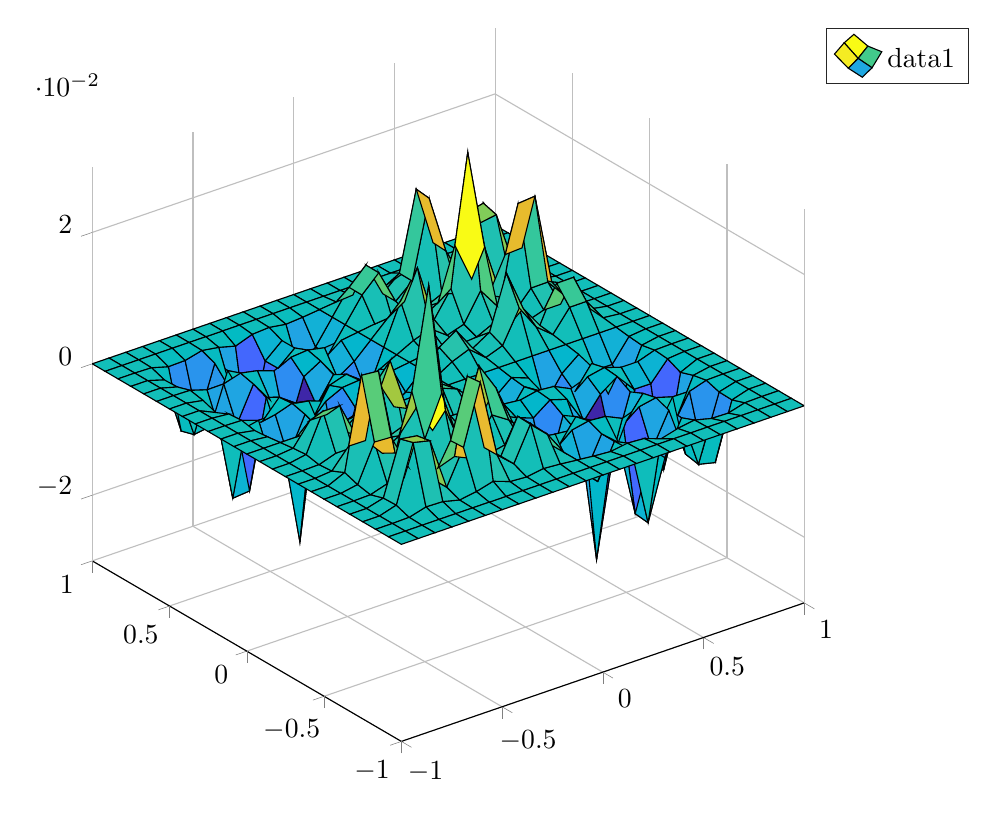
\begin{tikzpicture}

\begin{axis}[%
width=3.56in,
height=3.566in,
at={(0.597in,0.481in)},
scale only axis,
xmin=-1,
xmax=1,
tick align=outside,
ymin=-1,
ymax=1,
zmin=-0.03,
zmax=0.03,
view={-37.5}{30},
axis background/.style={fill=white},
axis x line*=bottom,
axis y line*=left,
axis z line*=left,
xmajorgrids,
ymajorgrids,
zmajorgrids,
legend style={at={(1.03,1)}, anchor=north west, legend cell align=left, align=left, draw=white!15!black}
]

\addplot3[%
surf,
shader=flat corner, draw=black, z buffer=sort, colormap={mymap}{[1pt] rgb(0pt)=(0.2422,0.1504,0.6603); rgb(1pt)=(0.25039,0.164995,0.707614); rgb(2pt)=(0.257771,0.181781,0.751138); rgb(3pt)=(0.264729,0.197757,0.795214); rgb(4pt)=(0.270648,0.214676,0.836371); rgb(5pt)=(0.275114,0.234238,0.870986); rgb(6pt)=(0.2783,0.255871,0.899071); rgb(7pt)=(0.280333,0.278233,0.9221); rgb(8pt)=(0.281338,0.300595,0.941376); rgb(9pt)=(0.281014,0.322757,0.957886); rgb(10pt)=(0.279467,0.344671,0.971676); rgb(11pt)=(0.275971,0.366681,0.982905); rgb(12pt)=(0.269914,0.3892,0.9906); rgb(13pt)=(0.260243,0.412329,0.995157); rgb(14pt)=(0.244033,0.435833,0.998833); rgb(15pt)=(0.220643,0.460257,0.997286); rgb(16pt)=(0.196333,0.484719,0.989152); rgb(17pt)=(0.183405,0.507371,0.979795); rgb(18pt)=(0.178643,0.528857,0.968157); rgb(19pt)=(0.176438,0.549905,0.952019); rgb(20pt)=(0.168743,0.570262,0.935871); rgb(21pt)=(0.154,0.5902,0.9218); rgb(22pt)=(0.146029,0.609119,0.907857); rgb(23pt)=(0.138024,0.627629,0.89729); rgb(24pt)=(0.124814,0.645929,0.888343); rgb(25pt)=(0.111252,0.6635,0.876314); rgb(26pt)=(0.0952095,0.679829,0.859781); rgb(27pt)=(0.0688714,0.694771,0.839357); rgb(28pt)=(0.0296667,0.708167,0.816333); rgb(29pt)=(0.00357143,0.720267,0.7917); rgb(30pt)=(0.00665714,0.731214,0.766014); rgb(31pt)=(0.0433286,0.741095,0.73941); rgb(32pt)=(0.0963952,0.75,0.712038); rgb(33pt)=(0.140771,0.7584,0.684157); rgb(34pt)=(0.1717,0.766962,0.655443); rgb(35pt)=(0.193767,0.775767,0.6251); rgb(36pt)=(0.216086,0.7843,0.5923); rgb(37pt)=(0.246957,0.791795,0.556743); rgb(38pt)=(0.290614,0.79729,0.518829); rgb(39pt)=(0.340643,0.8008,0.478857); rgb(40pt)=(0.3909,0.802871,0.435448); rgb(41pt)=(0.445629,0.802419,0.390919); rgb(42pt)=(0.5044,0.7993,0.348); rgb(43pt)=(0.561562,0.794233,0.304481); rgb(44pt)=(0.617395,0.787619,0.261238); rgb(45pt)=(0.671986,0.779271,0.2227); rgb(46pt)=(0.7242,0.769843,0.191029); rgb(47pt)=(0.773833,0.759805,0.16461); rgb(48pt)=(0.820314,0.749814,0.153529); rgb(49pt)=(0.863433,0.7406,0.159633); rgb(50pt)=(0.903543,0.733029,0.177414); rgb(51pt)=(0.939257,0.728786,0.209957); rgb(52pt)=(0.972757,0.729771,0.239443); rgb(53pt)=(0.995648,0.743371,0.237148); rgb(54pt)=(0.996986,0.765857,0.219943); rgb(55pt)=(0.995205,0.789252,0.202762); rgb(56pt)=(0.9892,0.813567,0.188533); rgb(57pt)=(0.978629,0.838629,0.176557); rgb(58pt)=(0.967648,0.8639,0.16429); rgb(59pt)=(0.96101,0.889019,0.153676); rgb(60pt)=(0.959671,0.913457,0.142257); rgb(61pt)=(0.962795,0.937338,0.12651); rgb(62pt)=(0.969114,0.960629,0.106362); rgb(63pt)=(0.9769,0.9839,0.0805)}, mesh/rows=25]
table[row sep=crcr, point meta=\thisrow{c}] {%
%
x	y	z	c\\
-1	-1	0	0\\
-0.916666666666667	-1	0	0\\
-0.833333333333333	-1	1.02695723625141e-24	1.02695723625141e-24\\
-0.75	-1	0	0\\
-0.666666666666667	-1	0	0\\
-0.583333333333333	-1	0	0\\
-0.5	-1	0	0\\
-0.416666666666667	-1	0	0\\
-0.333333333333333	-1	0	0\\
-0.25	-1	0	0\\
-0.166666666666667	-1	0	0\\
-0.0833333333333334	-1	0	0\\
0	-1	0	0\\
0.0833333333333333	-1	0	0\\
0.166666666666667	-1	0	0\\
0.25	-1	0	0\\
0.333333333333333	-1	0	0\\
0.416666666666667	-1	0	0\\
0.5	-1	0	0\\
0.583333333333333	-1	0	0\\
0.666666666666667	-1	0	0\\
0.75	-1	0	0\\
0.833333333333333	-1	0	0\\
0.916666666666667	-1	-4.38399307163469e-27	-4.38399307163469e-27\\
1	-1	0	0\\
-1	-0.916666666666667	0	0\\
-0.916666666666667	-0.916666666666667	2.55753406345044e-09	2.55753406345044e-09\\
-0.833333333333333	-0.916666666666667	3.85777718973534e-07	3.85777718973534e-07\\
-0.75	-0.916666666666667	4.17100875631788e-06	4.17100875631788e-06\\
-0.666666666666667	-0.916666666666667	3.64929550800072e-06	3.64929550800072e-06\\
-0.583333333333333	-0.916666666666667	3.45860111752149e-07	3.45860111752149e-07\\
-0.5	-0.916666666666667	2.33954300020683e-06	2.33954300020683e-06\\
-0.416666666666667	-0.916666666666667	5.70854139583692e-06	5.70854139583692e-06\\
-0.333333333333333	-0.916666666666667	1.17920908563584e-06	1.17920908563584e-06\\
-0.25	-0.916666666666667	3.45029265806706e-07	3.45029265806706e-07\\
-0.166666666666667	-0.916666666666667	2.26755661545572e-06	2.26755661545572e-06\\
-0.0833333333333334	-0.916666666666667	1.33785564740444e-06	1.33785564740444e-06\\
0	-0.916666666666667	-4.2425755489483e-22	-4.2425755489483e-22\\
0.0833333333333333	-0.916666666666667	-1.33785564740444e-06	-1.33785564740444e-06\\
0.166666666666667	-0.916666666666667	-2.26755661545571e-06	-2.26755661545571e-06\\
0.25	-0.916666666666667	-3.45029265806705e-07	-3.45029265806705e-07\\
0.333333333333333	-0.916666666666667	-1.17920908563584e-06	-1.17920908563584e-06\\
0.416666666666667	-0.916666666666667	-5.70854139583693e-06	-5.70854139583693e-06\\
0.5	-0.916666666666667	-2.33954300020683e-06	-2.33954300020683e-06\\
0.583333333333333	-0.916666666666667	-3.4586011175215e-07	-3.4586011175215e-07\\
0.666666666666667	-0.916666666666667	-3.64929550800072e-06	-3.64929550800072e-06\\
0.75	-0.916666666666667	-4.17100875631788e-06	-4.17100875631788e-06\\
0.833333333333333	-0.916666666666667	-3.85777718973533e-07	-3.85777718973533e-07\\
0.916666666666667	-0.916666666666667	-2.55753406345042e-09	-2.55753406345042e-09\\
1	-0.916666666666667	0	0\\
-1	-0.833333333333333	1.02695723625141e-24	1.02695723625141e-24\\
-0.916666666666667	-0.833333333333333	3.85777718973533e-07	3.85777718973533e-07\\
-0.833333333333333	-0.833333333333333	6.71198962422951e-05	6.71198962422951e-05\\
-0.75	-0.833333333333333	0.000778127800887982	0.000778127800887982\\
-0.666666666666667	-0.833333333333333	0.000707315736756557	0.000707315736756557\\
-0.583333333333333	-0.833333333333333	6.86074746915453e-05	6.86074746915453e-05\\
-0.5	-0.833333333333333	0.000471138162446881	0.000471138162446881\\
-0.416666666666667	-0.833333333333333	0.00116140316014542	0.00116140316014542\\
-0.333333333333333	-0.833333333333333	0.000241610914204461	0.000241610914204461\\
-0.25	-0.833333333333333	7.10368896279139e-05	7.10368896279139e-05\\
-0.166666666666667	-0.833333333333333	0.000468336406285743	0.000468336406285743\\
-0.0833333333333334	-0.833333333333333	0.000276812375771035	0.000276812375771035\\
0	-0.833333333333333	-7.74552301490904e-20	-7.74552301490904e-20\\
0.0833333333333333	-0.833333333333333	-0.000276812375771035	-0.000276812375771035\\
0.166666666666667	-0.833333333333333	-0.000468336406285742	-0.000468336406285742\\
0.25	-0.833333333333333	-7.10368896279136e-05	-7.10368896279136e-05\\
0.333333333333333	-0.833333333333333	-0.00024161091420446	-0.00024161091420446\\
0.416666666666667	-0.833333333333333	-0.00116140316014542	-0.00116140316014542\\
0.5	-0.833333333333333	-0.000471138162446881	-0.000471138162446881\\
0.583333333333333	-0.833333333333333	-6.86074746915456e-05	-6.86074746915456e-05\\
0.666666666666667	-0.833333333333333	-0.000707315736756559	-0.000707315736756559\\
0.75	-0.833333333333333	-0.000778127800887981	-0.000778127800887981\\
0.833333333333333	-0.833333333333333	-6.7119896242295e-05	-6.7119896242295e-05\\
0.916666666666667	-0.833333333333333	-3.85777718973525e-07	-3.85777718973525e-07\\
1	-0.833333333333333	-1.0269572362514e-24	-1.0269572362514e-24\\
-1	-0.75	0	0\\
-0.916666666666667	-0.75	4.17100875631788e-06	4.17100875631788e-06\\
-0.833333333333333	-0.75	0.000778127800887983	0.000778127800887983\\
-0.75	-0.75	0.00943571698715445	0.00943571698715445\\
-0.666666666666667	-0.75	0.00882480124123988	0.00882480124123988\\
-0.583333333333333	-0.75	0.000872104526134152	0.000872104526134152\\
-0.5	-0.75	0.0060652983794619	0.0060652983794619\\
-0.416666666666667	-0.75	0.0150841772008774	0.0150841772008774\\
-0.333333333333333	-0.75	0.00315753528677166	0.00315753528677166\\
-0.25	-0.75	0.000932352964394895	0.000932352964394895\\
-0.166666666666667	-0.75	0.00616423466770155	0.00616423466770155\\
-0.0833333333333334	-0.75	0.00364924259814257	0.00364924259814257\\
0	-0.75	-8.76737641779841e-19	-8.76737641779841e-19\\
0.0833333333333333	-0.75	-0.00364924259814257	-0.00364924259814257\\
0.166666666666667	-0.75	-0.00616423466770154	-0.00616423466770154\\
0.25	-0.75	-0.000932352964394891	-0.000932352964394891\\
0.333333333333333	-0.75	-0.00315753528677164	-0.00315753528677164\\
0.416666666666667	-0.75	-0.0150841772008774	-0.0150841772008774\\
0.5	-0.75	-0.0060652983794619	-0.0060652983794619\\
0.583333333333333	-0.75	-0.000872104526134156	-0.000872104526134156\\
0.666666666666667	-0.75	-0.00882480124123989	-0.00882480124123989\\
0.75	-0.75	-0.00943571698715444	-0.00943571698715444\\
0.833333333333333	-0.75	-0.000778127800887982	-0.000778127800887982\\
0.916666666666667	-0.75	-4.17100875631781e-06	-4.17100875631781e-06\\
1	-0.75	0	0\\
-1	-0.666666666666667	0	0\\
-0.916666666666667	-0.666666666666667	3.64929550800072e-06	3.64929550800072e-06\\
-0.833333333333333	-0.666666666666667	0.000707315736756557	0.000707315736756557\\
-0.75	-0.666666666666667	0.00882480124123988	0.00882480124123988\\
-0.666666666666667	-0.666666666666667	0.00842066215543398	0.00842066215543398\\
-0.583333333333333	-0.666666666666667	0.000843966898384536	0.000843966898384536\\
-0.5	-0.666666666666667	0.00592857826938018	0.00592857826938018\\
-0.416666666666667	-0.666666666666667	0.0148502404760497	0.0148502404760497\\
-0.333333333333333	-0.666666666666667	0.00312456184123599	0.00312456184123599\\
-0.25	-0.666666666666667	0.000925942478032866	0.000925942478032866\\
-0.166666666666667	-0.666666666666667	0.00613646636398126	0.00613646636398126\\
-0.0833333333333334	-0.666666666666667	0.00363775449063844	0.00363775449063844\\
0	-0.666666666666667	-8.44331861748012e-19	-8.44331861748012e-19\\
0.0833333333333333	-0.666666666666667	-0.00363775449063844	-0.00363775449063844\\
0.166666666666667	-0.666666666666667	-0.00613646636398124	-0.00613646636398124\\
0.25	-0.666666666666667	-0.000925942478032862	-0.000925942478032862\\
0.333333333333333	-0.666666666666667	-0.00312456184123597	-0.00312456184123597\\
0.416666666666667	-0.666666666666667	-0.0148502404760497	-0.0148502404760497\\
0.5	-0.666666666666667	-0.00592857826938018	-0.00592857826938018\\
0.583333333333333	-0.666666666666667	-0.00084396689838454	-0.00084396689838454\\
0.666666666666667	-0.666666666666667	-0.00842066215543399	-0.00842066215543399\\
0.75	-0.666666666666667	-0.00882480124123987	-0.00882480124123987\\
0.833333333333333	-0.666666666666667	-0.000707315736756558	-0.000707315736756558\\
0.916666666666667	-0.666666666666667	-3.64929550800066e-06	-3.64929550800066e-06\\
1	-0.666666666666667	0	0\\
-1	-0.583333333333333	0	0\\
-0.916666666666667	-0.583333333333333	3.45860111752149e-07	3.45860111752149e-07\\
-0.833333333333333	-0.583333333333333	6.86074746915453e-05	6.86074746915453e-05\\
-0.75	-0.583333333333333	0.000872104526134152	0.000872104526134152\\
-0.666666666666667	-0.583333333333333	0.000843966898384536	0.000843966898384536\\
-0.583333333333333	-0.583333333333333	8.50681297213606e-05	8.50681297213606e-05\\
-0.5	-0.583333333333333	0.000592761470027727	0.000592761470027727\\
-0.416666666666667	-0.583333333333333	0.00149315597727987	0.00149315597727987\\
-0.333333333333333	-0.583333333333333	0.000315453871556334	0.000315453871556334\\
-0.25	-0.583333333333333	9.31814902686496e-05	9.31814902686496e-05\\
-0.166666666666667	-0.583333333333333	0.000618502248354859	0.000618502248354859\\
-0.0833333333333334	-0.583333333333333	0.000367064223668659	0.000367064223668659\\
0	-0.583333333333333	-7.40930762219607e-20	-7.40930762219607e-20\\
0.0833333333333333	-0.583333333333333	-0.000367064223668659	-0.000367064223668659\\
0.166666666666667	-0.583333333333333	-0.000618502248354857	-0.000618502248354857\\
0.25	-0.583333333333333	-9.31814902686491e-05	-9.31814902686491e-05\\
0.333333333333333	-0.583333333333333	-0.000315453871556332	-0.000315453871556332\\
0.416666666666667	-0.583333333333333	-0.00149315597727987	-0.00149315597727987\\
0.5	-0.583333333333333	-0.000592761470027727	-0.000592761470027727\\
0.583333333333333	-0.583333333333333	-8.50681297213611e-05	-8.50681297213611e-05\\
0.666666666666667	-0.583333333333333	-0.000843966898384538	-0.000843966898384538\\
0.75	-0.583333333333333	-0.00087210452613415	-0.00087210452613415\\
0.833333333333333	-0.583333333333333	-6.86074746915454e-05	-6.86074746915454e-05\\
0.916666666666667	-0.583333333333333	-3.45860111752143e-07	-3.45860111752143e-07\\
1	-0.583333333333333	0	0\\
-1	-0.5	0	0\\
-0.916666666666667	-0.5	2.33954300020683e-06	2.33954300020683e-06\\
-0.833333333333333	-0.5	0.000471138162446881	0.000471138162446881\\
-0.75	-0.5	0.0060652983794619	0.0060652983794619\\
-0.666666666666667	-0.5	0.00592857826938018	0.00592857826938018\\
-0.583333333333333	-0.5	0.000592761470027727	0.000592761470027727\\
-0.5	-0.5	0.00393294666281547	0.00393294666281547\\
-0.416666666666667	-0.5	0.00994977833558941	0.00994977833558941\\
-0.333333333333333	-0.5	0.00210867680461956	0.00210867680461956\\
-0.25	-0.5	0.000610455051438689	0.000610455051438689\\
-0.166666666666667	-0.5	0.00405241439845992	0.00405241439845992\\
-0.0833333333333334	-0.5	0.0024071556172955	0.0024071556172955\\
0	-0.5	-5.91805759022251e-19	-5.91805759022251e-19\\
0.0833333333333333	-0.5	-0.0024071556172955	-0.0024071556172955\\
0.166666666666667	-0.5	-0.00405241439845991	-0.00405241439845991\\
0.25	-0.5	-0.000610455051438686	-0.000610455051438686\\
0.333333333333333	-0.5	-0.00210867680461956	-0.00210867680461956\\
0.416666666666667	-0.5	-0.00994977833558942	-0.00994977833558942\\
0.5	-0.5	-0.00393294666281547	-0.00393294666281547\\
0.583333333333333	-0.5	-0.000592761470027729	-0.000592761470027729\\
0.666666666666667	-0.5	-0.00592857826938019	-0.00592857826938019\\
0.75	-0.5	-0.00606529837946189	-0.00606529837946189\\
0.833333333333333	-0.5	-0.000471138162446881	-0.000471138162446881\\
0.916666666666667	-0.5	-2.33954300020679e-06	-2.33954300020679e-06\\
1	-0.5	0	0\\
-1	-0.416666666666667	0	0\\
-0.916666666666667	-0.416666666666667	5.70854139583692e-06	5.70854139583692e-06\\
-0.833333333333333	-0.416666666666667	0.00116140316014542	0.00116140316014542\\
-0.75	-0.416666666666667	0.0150841772008774	0.0150841772008774\\
-0.666666666666667	-0.416666666666667	0.0148502404760497	0.0148502404760497\\
-0.583333333333333	-0.416666666666667	0.00149315597727987	0.00149315597727987\\
-0.5	-0.416666666666667	0.00994977833558941	0.00994977833558941\\
-0.416666666666667	-0.416666666666667	0.0252552578198303	0.0252552578198303\\
-0.333333333333333	-0.416666666666667	0.00536572588063085	0.00536572588063085\\
-0.25	-0.416666666666667	0.00155612453270233	0.00155612453270233\\
-0.166666666666667	-0.416666666666667	0.010342674976464	0.010342674976464\\
-0.0833333333333334	-0.416666666666667	0.00614793627719881	0.00614793627719881\\
0	-0.416666666666667	-1.50433859765667e-18	-1.50433859765667e-18\\
0.0833333333333333	-0.416666666666667	-0.0061479362771988	-0.0061479362771988\\
0.166666666666667	-0.416666666666667	-0.010342674976464	-0.010342674976464\\
0.25	-0.416666666666667	-0.00155612453270232	-0.00155612453270232\\
0.333333333333333	-0.416666666666667	-0.00536572588063083	-0.00536572588063083\\
0.416666666666667	-0.416666666666667	-0.0252552578198304	-0.0252552578198304\\
0.5	-0.416666666666667	-0.00994977833558941	-0.00994977833558941\\
0.583333333333333	-0.416666666666667	-0.00149315597727988	-0.00149315597727988\\
0.666666666666667	-0.416666666666667	-0.0148502404760497	-0.0148502404760497\\
0.75	-0.416666666666667	-0.0150841772008774	-0.0150841772008774\\
0.833333333333333	-0.416666666666667	-0.00116140316014542	-0.00116140316014542\\
0.916666666666667	-0.416666666666667	-5.70854139583682e-06	-5.70854139583682e-06\\
1	-0.416666666666667	0	0\\
-1	-0.333333333333333	0	0\\
-0.916666666666667	-0.333333333333333	1.17920908563584e-06	1.17920908563584e-06\\
-0.833333333333333	-0.333333333333333	0.000241610914204461	0.000241610914204461\\
-0.75	-0.333333333333333	0.00315753528677166	0.00315753528677166\\
-0.666666666666667	-0.333333333333333	0.00312456184123599	0.00312456184123599\\
-0.583333333333333	-0.333333333333333	0.000315453871556334	0.000315453871556334\\
-0.5	-0.333333333333333	0.00210867680461956	0.00210867680461956\\
-0.416666666666667	-0.333333333333333	0.00536572588063085	0.00536572588063085\\
-0.333333333333333	-0.333333333333333	0.00114214387023767	0.00114214387023767\\
-0.25	-0.333333333333333	0.000331677317790113	0.000331677317790113\\
-0.166666666666667	-0.333333333333333	0.00220651736235955	0.00220651736235955\\
-0.0833333333333334	-0.333333333333333	0.00131231582712499	0.00131231582712499\\
0	-0.333333333333333	-3.16585135024486e-19	-3.16585135024486e-19\\
0.0833333333333333	-0.333333333333333	-0.00131231582712499	-0.00131231582712499\\
0.166666666666667	-0.333333333333333	-0.00220651736235954	-0.00220651736235954\\
0.25	-0.333333333333333	-0.000331677317790112	-0.000331677317790112\\
0.333333333333333	-0.333333333333333	-0.00114214387023766	-0.00114214387023766\\
0.416666666666667	-0.333333333333333	-0.00536572588063086	-0.00536572588063086\\
0.5	-0.333333333333333	-0.00210867680461956	-0.00210867680461956\\
0.583333333333333	-0.333333333333333	-0.000315453871556335	-0.000315453871556335\\
0.666666666666667	-0.333333333333333	-0.00312456184123599	-0.00312456184123599\\
0.75	-0.333333333333333	-0.00315753528677165	-0.00315753528677165\\
0.833333333333333	-0.333333333333333	-0.000241610914204461	-0.000241610914204461\\
0.916666666666667	-0.333333333333333	-1.17920908563582e-06	-1.17920908563582e-06\\
1	-0.333333333333333	0	0\\
-1	-0.25	0	0\\
-0.916666666666667	-0.25	3.45029265806706e-07	3.45029265806706e-07\\
-0.833333333333333	-0.25	7.1036889627914e-05	7.1036889627914e-05\\
-0.75	-0.25	0.000932352964394894	0.000932352964394894\\
-0.666666666666667	-0.25	0.000925942478032866	0.000925942478032866\\
-0.583333333333333	-0.25	9.31814902686495e-05	9.31814902686495e-05\\
-0.5	-0.25	0.000610455051438689	0.000610455051438689\\
-0.416666666666667	-0.25	0.00155612453270233	0.00155612453270233\\
-0.333333333333333	-0.25	0.000331677317790113	0.000331677317790113\\
-0.25	-0.25	9.54350634367825e-05	9.54350634367825e-05\\
-0.166666666666667	-0.25	0.000634901021554919	0.000634901021554919\\
-0.0833333333333334	-0.25	0.00037775454883306	0.00037775454883306\\
0	-0.25	-8.80499813311504e-20	-8.80499813311504e-20\\
0.0833333333333333	-0.25	-0.00037775454883306	-0.00037775454883306\\
0.166666666666667	-0.25	-0.000634901021554917	-0.000634901021554917\\
0.25	-0.25	-9.54350634367821e-05	-9.54350634367821e-05\\
0.333333333333333	-0.25	-0.000331677317790112	-0.000331677317790112\\
0.416666666666667	-0.25	-0.00155612453270233	-0.00155612453270233\\
0.5	-0.25	-0.000610455051438689	-0.000610455051438689\\
0.583333333333333	-0.25	-9.31814902686498e-05	-9.31814902686498e-05\\
0.666666666666667	-0.25	-0.000925942478032867	-0.000925942478032867\\
0.75	-0.25	-0.000932352964394893	-0.000932352964394893\\
0.833333333333333	-0.25	-7.1036889627914e-05	-7.1036889627914e-05\\
0.916666666666667	-0.25	-3.450292658067e-07	-3.450292658067e-07\\
1	-0.25	0	0\\
-1	-0.166666666666667	0	0\\
-0.916666666666667	-0.166666666666667	2.26755661545572e-06	2.26755661545572e-06\\
-0.833333333333333	-0.166666666666667	0.000468336406285743	0.000468336406285743\\
-0.75	-0.166666666666667	0.00616423466770155	0.00616423466770155\\
-0.666666666666667	-0.166666666666667	0.00613646636398126	0.00613646636398126\\
-0.583333333333333	-0.166666666666667	0.000618502248354858	0.000618502248354858\\
-0.5	-0.166666666666667	0.00405241439845992	0.00405241439845992\\
-0.416666666666667	-0.166666666666667	0.010342674976464	0.010342674976464\\
-0.333333333333333	-0.166666666666667	0.00220651736235955	0.00220651736235955\\
-0.25	-0.166666666666667	0.000634901021554919	0.000634901021554919\\
-0.166666666666667	-0.166666666666667	0.00422559650685534	0.00422559650685534\\
-0.0833333333333334	-0.166666666666667	0.00251483803933617	0.00251483803933617\\
0	-0.166666666666667	-6.34758211468699e-19	-6.34758211468699e-19\\
0.0833333333333333	-0.166666666666667	-0.00251483803933617	-0.00251483803933617\\
0.166666666666667	-0.166666666666667	-0.00422559650685533	-0.00422559650685533\\
0.25	-0.166666666666667	-0.000634901021554916	-0.000634901021554916\\
0.333333333333333	-0.166666666666667	-0.00220651736235954	-0.00220651736235954\\
0.416666666666667	-0.166666666666667	-0.010342674976464	-0.010342674976464\\
0.5	-0.166666666666667	-0.00405241439845992	-0.00405241439845992\\
0.583333333333333	-0.166666666666667	-0.000618502248354861	-0.000618502248354861\\
0.666666666666667	-0.166666666666667	-0.00613646636398127	-0.00613646636398127\\
0.75	-0.166666666666667	-0.00616423466770154	-0.00616423466770154\\
0.833333333333333	-0.166666666666667	-0.000468336406285743	-0.000468336406285743\\
0.916666666666667	-0.166666666666667	-2.26755661545568e-06	-2.26755661545568e-06\\
1	-0.166666666666667	0	0\\
-1	-0.0833333333333334	0	0\\
-0.916666666666667	-0.0833333333333334	1.33785564740444e-06	1.33785564740444e-06\\
-0.833333333333333	-0.0833333333333334	0.000276812375771035	0.000276812375771035\\
-0.75	-0.0833333333333334	0.00364924259814257	0.00364924259814257\\
-0.666666666666667	-0.0833333333333334	0.00363775449063844	0.00363775449063844\\
-0.583333333333333	-0.0833333333333334	0.000367064223668659	0.000367064223668659\\
-0.5	-0.0833333333333334	0.0024071556172955	0.0024071556172955\\
-0.416666666666667	-0.0833333333333334	0.0061479362771988	0.0061479362771988\\
-0.333333333333333	-0.0833333333333334	0.00131231582712499	0.00131231582712499\\
-0.25	-0.0833333333333334	0.00037775454883306	0.00037775454883306\\
-0.166666666666667	-0.0833333333333334	0.00251483803933617	0.00251483803933617\\
-0.0833333333333334	-0.0833333333333334	0.0014969284339611	0.0014969284339611\\
0	-0.0833333333333334	-4.12134423225633e-19	-4.12134423225633e-19\\
0.0833333333333333	-0.0833333333333334	-0.0014969284339611	-0.0014969284339611\\
0.166666666666667	-0.0833333333333334	-0.00251483803933616	-0.00251483803933616\\
0.25	-0.0833333333333334	-0.000377754548833058	-0.000377754548833058\\
0.333333333333333	-0.0833333333333334	-0.00131231582712498	-0.00131231582712498\\
0.416666666666667	-0.0833333333333334	-0.00614793627719881	-0.00614793627719881\\
0.5	-0.0833333333333334	-0.00240715561729551	-0.00240715561729551\\
0.583333333333333	-0.0833333333333334	-0.000367064223668661	-0.000367064223668661\\
0.666666666666667	-0.0833333333333334	-0.00363775449063844	-0.00363775449063844\\
0.75	-0.0833333333333334	-0.00364924259814256	-0.00364924259814256\\
0.833333333333333	-0.0833333333333334	-0.000276812375771035	-0.000276812375771035\\
0.916666666666667	-0.0833333333333334	-1.33785564740442e-06	-1.33785564740442e-06\\
1	-0.0833333333333334	0	0\\
-1	0	0	0\\
-0.916666666666667	0	-4.22019650749432e-22	-4.22019650749432e-22\\
-0.833333333333333	0	-7.58062703141482e-20	-7.58062703141482e-20\\
-0.75	0	-8.8948973557021e-19	-8.8948973557021e-19\\
-0.666666666666667	0	-8.48925864908015e-19	-8.48925864908015e-19\\
-0.583333333333333	0	-7.4663668535476e-20	-7.4663668535476e-20\\
-0.5	0	-6.59299545930563e-19	-6.59299545930563e-19\\
-0.416666666666667	0	-1.65655633099897e-18	-1.65655633099897e-18\\
-0.333333333333333	0	-3.57084812293917e-19	-3.57084812293917e-19\\
-0.25	0	-8.37743870326049e-20	-8.37743870326049e-20\\
-0.166666666666667	0	-6.03879200828298e-19	-6.03879200828298e-19\\
-0.0833333333333334	0	-3.932851103973e-19	-3.932851103973e-19\\
0	0	-4.82118586296267e-21	-4.82118586296267e-21\\
0.0833333333333333	0	4.48056541275829e-19	4.48056541275829e-19\\
0.166666666666667	0	6.75165917404855e-19	6.75165917404855e-19\\
0.25	0	8.05379513898792e-20	8.05379513898792e-20\\
0.333333333333333	0	3.00487456194101e-19	3.00487456194101e-19\\
0.416666666666667	0	1.62580333661468e-18	1.62580333661468e-18\\
0.5	0	5.57212921187685e-19	5.57212921187685e-19\\
0.583333333333333	0	9.80093456331336e-20	9.80093456331336e-20\\
0.666666666666667	0	8.61737011716055e-19	8.61737011716055e-19\\
0.75	0	9.60761298722394e-19	9.60761298722394e-19\\
0.833333333333333	0	7.99192795843061e-20	7.99192795843061e-20\\
0.916666666666667	0	3.15236993062634e-22	3.15236993062634e-22\\
1	0	0	0\\
-1	0.0833333333333333	0	0\\
-0.916666666666667	0.0833333333333333	-1.33785564740444e-06	-1.33785564740444e-06\\
-0.833333333333333	0.0833333333333333	-0.000276812375771035	-0.000276812375771035\\
-0.75	0.0833333333333333	-0.00364924259814257	-0.00364924259814257\\
-0.666666666666667	0.0833333333333333	-0.00363775449063844	-0.00363775449063844\\
-0.583333333333333	0.0833333333333333	-0.000367064223668659	-0.000367064223668659\\
-0.5	0.0833333333333333	-0.0024071556172955	-0.0024071556172955\\
-0.416666666666667	0.0833333333333333	-0.0061479362771988	-0.0061479362771988\\
-0.333333333333333	0.0833333333333333	-0.00131231582712499	-0.00131231582712499\\
-0.25	0.0833333333333333	-0.00037775454883306	-0.00037775454883306\\
-0.166666666666667	0.0833333333333333	-0.00251483803933617	-0.00251483803933617\\
-0.0833333333333334	0.0833333333333333	-0.0014969284339611	-0.0014969284339611\\
0	0.0833333333333333	4.51410925247731e-19	4.51410925247731e-19\\
0.0833333333333333	0.0833333333333333	0.0014969284339611	0.0014969284339611\\
0.166666666666667	0.0833333333333333	0.00251483803933616	0.00251483803933616\\
0.25	0.0833333333333333	0.000377754548833058	0.000377754548833058\\
0.333333333333333	0.0833333333333333	0.00131231582712498	0.00131231582712498\\
0.416666666666667	0.0833333333333333	0.00614793627719881	0.00614793627719881\\
0.5	0.0833333333333333	0.0024071556172955	0.0024071556172955\\
0.583333333333333	0.0833333333333333	0.00036706422366866	0.00036706422366866\\
0.666666666666667	0.0833333333333333	0.00363775449063844	0.00363775449063844\\
0.75	0.0833333333333333	0.00364924259814256	0.00364924259814256\\
0.833333333333333	0.0833333333333333	0.000276812375771035	0.000276812375771035\\
0.916666666666667	0.0833333333333333	1.33785564740442e-06	1.33785564740442e-06\\
1	0.0833333333333333	0	0\\
-1	0.166666666666667	0	0\\
-0.916666666666667	0.166666666666667	-2.26755661545571e-06	-2.26755661545571e-06\\
-0.833333333333333	0.166666666666667	-0.000468336406285741	-0.000468336406285741\\
-0.75	0.166666666666667	-0.00616423466770153	-0.00616423466770153\\
-0.666666666666667	0.166666666666667	-0.00613646636398124	-0.00613646636398124\\
-0.583333333333333	0.166666666666667	-0.000618502248354857	-0.000618502248354857\\
-0.5	0.166666666666667	-0.00405241439845991	-0.00405241439845991\\
-0.416666666666667	0.166666666666667	-0.010342674976464	-0.010342674976464\\
-0.333333333333333	0.166666666666667	-0.00220651736235954	-0.00220651736235954\\
-0.25	0.166666666666667	-0.000634901021554917	-0.000634901021554917\\
-0.166666666666667	0.166666666666667	-0.00422559650685533	-0.00422559650685533\\
-0.0833333333333334	0.166666666666667	-0.00251483803933616	-0.00251483803933616\\
0	0.166666666666667	6.9848421185914e-19	6.9848421185914e-19\\
0.0833333333333333	0.166666666666667	0.00251483803933616	0.00251483803933616\\
0.166666666666667	0.166666666666667	0.00422559650685532	0.00422559650685532\\
0.25	0.166666666666667	0.000634901021554914	0.000634901021554914\\
0.333333333333333	0.166666666666667	0.00220651736235953	0.00220651736235953\\
0.416666666666667	0.166666666666667	0.010342674976464	0.010342674976464\\
0.5	0.166666666666667	0.00405241439845991	0.00405241439845991\\
0.583333333333333	0.166666666666667	0.000618502248354859	0.000618502248354859\\
0.666666666666667	0.166666666666667	0.00613646636398125	0.00613646636398125\\
0.75	0.166666666666667	0.00616423466770152	0.00616423466770152\\
0.833333333333333	0.166666666666667	0.000468336406285741	0.000468336406285741\\
0.916666666666667	0.166666666666667	2.26755661545567e-06	2.26755661545567e-06\\
1	0.166666666666667	0	0\\
-1	0.25	0	0\\
-0.916666666666667	0.25	-3.45029265806704e-07	-3.45029265806704e-07\\
-0.833333333333333	0.25	-7.10368896279136e-05	-7.10368896279136e-05\\
-0.75	0.25	-0.000932352964394891	-0.000932352964394891\\
-0.666666666666667	0.25	-0.000925942478032862	-0.000925942478032862\\
-0.583333333333333	0.25	-9.31814902686491e-05	-9.31814902686491e-05\\
-0.5	0.25	-0.000610455051438686	-0.000610455051438686\\
-0.416666666666667	0.25	-0.00155612453270232	-0.00155612453270232\\
-0.333333333333333	0.25	-0.000331677317790112	-0.000331677317790112\\
-0.25	0.25	-9.5435063436782e-05	-9.5435063436782e-05\\
-0.166666666666667	0.25	-0.000634901021554916	-0.000634901021554916\\
-0.0833333333333334	0.25	-0.000377754548833058	-0.000377754548833058\\
0	0.25	7.94089675468141e-20	7.94089675468141e-20\\
0.0833333333333333	0.25	0.000377754548833058	0.000377754548833058\\
0.166666666666667	0.25	0.000634901021554914	0.000634901021554914\\
0.25	0.25	9.54350634367817e-05	9.54350634367817e-05\\
0.333333333333333	0.25	0.000331677317790111	0.000331677317790111\\
0.416666666666667	0.25	0.00155612453270232	0.00155612453270232\\
0.5	0.25	0.000610455051438686	0.000610455051438686\\
0.583333333333333	0.25	9.31814902686495e-05	9.31814902686495e-05\\
0.666666666666667	0.25	0.000925942478032864	0.000925942478032864\\
0.75	0.25	0.000932352964394889	0.000932352964394889\\
0.833333333333333	0.25	7.10368896279137e-05	7.10368896279137e-05\\
0.916666666666667	0.25	3.45029265806699e-07	3.45029265806699e-07\\
1	0.25	0	0\\
-1	0.333333333333333	0	0\\
-0.916666666666667	0.333333333333333	-1.17920908563583e-06	-1.17920908563583e-06\\
-0.833333333333333	0.333333333333333	-0.00024161091420446	-0.00024161091420446\\
-0.75	0.333333333333333	-0.00315753528677164	-0.00315753528677164\\
-0.666666666666667	0.333333333333333	-0.00312456184123597	-0.00312456184123597\\
-0.583333333333333	0.333333333333333	-0.000315453871556332	-0.000315453871556332\\
-0.5	0.333333333333333	-0.00210867680461956	-0.00210867680461956\\
-0.416666666666667	0.333333333333333	-0.00536572588063083	-0.00536572588063083\\
-0.333333333333333	0.333333333333333	-0.00114214387023766	-0.00114214387023766\\
-0.25	0.333333333333333	-0.000331677317790112	-0.000331677317790112\\
-0.166666666666667	0.333333333333333	-0.00220651736235954	-0.00220651736235954\\
-0.0833333333333334	0.333333333333333	-0.00131231582712498	-0.00131231582712498\\
0	0.333333333333333	3.22485562489602e-19	3.22485562489602e-19\\
0.0833333333333333	0.333333333333333	0.00131231582712498	0.00131231582712498\\
0.166666666666667	0.333333333333333	0.00220651736235953	0.00220651736235953\\
0.25	0.333333333333333	0.000331677317790111	0.000331677317790111\\
0.333333333333333	0.333333333333333	0.00114214387023766	0.00114214387023766\\
0.416666666666667	0.333333333333333	0.00536572588063084	0.00536572588063084\\
0.5	0.333333333333333	0.00210867680461956	0.00210867680461956\\
0.583333333333333	0.333333333333333	0.000315453871556334	0.000315453871556334\\
0.666666666666667	0.333333333333333	0.00312456184123598	0.00312456184123598\\
0.75	0.333333333333333	0.00315753528677164	0.00315753528677164\\
0.833333333333333	0.333333333333333	0.00024161091420446	0.00024161091420446\\
0.916666666666667	0.333333333333333	1.17920908563582e-06	1.17920908563582e-06\\
1	0.333333333333333	0	0\\
-1	0.416666666666667	0	0\\
-0.916666666666667	0.416666666666667	-5.70854139583693e-06	-5.70854139583693e-06\\
-0.833333333333333	0.416666666666667	-0.00116140316014542	-0.00116140316014542\\
-0.75	0.416666666666667	-0.0150841772008774	-0.0150841772008774\\
-0.666666666666667	0.416666666666667	-0.0148502404760497	-0.0148502404760497\\
-0.583333333333333	0.416666666666667	-0.00149315597727987	-0.00149315597727987\\
-0.5	0.416666666666667	-0.00994977833558942	-0.00994977833558942\\
-0.416666666666667	0.416666666666667	-0.0252552578198304	-0.0252552578198304\\
-0.333333333333333	0.416666666666667	-0.00536572588063086	-0.00536572588063086\\
-0.25	0.416666666666667	-0.00155612453270233	-0.00155612453270233\\
-0.166666666666667	0.416666666666667	-0.010342674976464	-0.010342674976464\\
-0.0833333333333334	0.416666666666667	-0.00614793627719881	-0.00614793627719881\\
0	0.416666666666667	1.70743447471519e-18	1.70743447471519e-18\\
0.0833333333333333	0.416666666666667	0.00614793627719881	0.00614793627719881\\
0.166666666666667	0.416666666666667	0.010342674976464	0.010342674976464\\
0.25	0.416666666666667	0.00155612453270232	0.00155612453270232\\
0.333333333333333	0.416666666666667	0.00536572588063084	0.00536572588063084\\
0.416666666666667	0.416666666666667	0.0252552578198304	0.0252552578198304\\
0.5	0.416666666666667	0.00994977833558942	0.00994977833558942\\
0.583333333333333	0.416666666666667	0.00149315597727988	0.00149315597727988\\
0.666666666666667	0.416666666666667	0.0148502404760497	0.0148502404760497\\
0.75	0.416666666666667	0.0150841772008774	0.0150841772008774\\
0.833333333333333	0.416666666666667	0.00116140316014542	0.00116140316014542\\
0.916666666666667	0.416666666666667	5.70854139583684e-06	5.70854139583684e-06\\
1	0.416666666666667	0	0\\
-1	0.5	0	0\\
-0.916666666666667	0.5	-2.33954300020683e-06	-2.33954300020683e-06\\
-0.833333333333333	0.5	-0.000471138162446881	-0.000471138162446881\\
-0.75	0.5	-0.0060652983794619	-0.0060652983794619\\
-0.666666666666667	0.5	-0.00592857826938018	-0.00592857826938018\\
-0.583333333333333	0.5	-0.000592761470027727	-0.000592761470027727\\
-0.5	0.5	-0.00393294666281547	-0.00393294666281547\\
-0.416666666666667	0.5	-0.00994977833558941	-0.00994977833558941\\
-0.333333333333333	0.5	-0.00210867680461956	-0.00210867680461956\\
-0.25	0.5	-0.000610455051438689	-0.000610455051438689\\
-0.166666666666667	0.5	-0.00405241439845992	-0.00405241439845992\\
-0.0833333333333334	0.5	-0.00240715561729551	-0.00240715561729551\\
0	0.5	5.92452022970232e-19	5.92452022970232e-19\\
0.0833333333333333	0.5	0.0024071556172955	0.0024071556172955\\
0.166666666666667	0.5	0.00405241439845991	0.00405241439845991\\
0.25	0.5	0.000610455051438686	0.000610455051438686\\
0.333333333333333	0.5	0.00210867680461956	0.00210867680461956\\
0.416666666666667	0.5	0.00994977833558942	0.00994977833558942\\
0.5	0.5	0.00393294666281547	0.00393294666281547\\
0.583333333333333	0.5	0.000592761470027729	0.000592761470027729\\
0.666666666666667	0.5	0.00592857826938019	0.00592857826938019\\
0.75	0.5	0.00606529837946189	0.00606529837946189\\
0.833333333333333	0.5	0.000471138162446881	0.000471138162446881\\
0.916666666666667	0.5	2.33954300020679e-06	2.33954300020679e-06\\
1	0.5	0	0\\
-1	0.583333333333333	0	0\\
-0.916666666666667	0.583333333333333	-3.45860111752151e-07	-3.45860111752151e-07\\
-0.833333333333333	0.583333333333333	-6.86074746915456e-05	-6.86074746915456e-05\\
-0.75	0.583333333333333	-0.000872104526134156	-0.000872104526134156\\
-0.666666666666667	0.583333333333333	-0.00084396689838454	-0.00084396689838454\\
-0.583333333333333	0.583333333333333	-8.50681297213611e-05	-8.50681297213611e-05\\
-0.5	0.583333333333333	-0.000592761470027729	-0.000592761470027729\\
-0.416666666666667	0.583333333333333	-0.00149315597727988	-0.00149315597727988\\
-0.333333333333333	0.583333333333333	-0.000315453871556335	-0.000315453871556335\\
-0.25	0.583333333333333	-9.31814902686498e-05	-9.31814902686498e-05\\
-0.166666666666667	0.583333333333333	-0.000618502248354861	-0.000618502248354861\\
-0.0833333333333334	0.583333333333333	-0.000367064223668661	-0.000367064223668661\\
0	0.583333333333333	1.04971725804411e-19	1.04971725804411e-19\\
0.0833333333333333	0.583333333333333	0.00036706422366866	0.00036706422366866\\
0.166666666666667	0.583333333333333	0.00061850224835486	0.00061850224835486\\
0.25	0.583333333333333	9.31814902686495e-05	9.31814902686495e-05\\
0.333333333333333	0.583333333333333	0.000315453871556334	0.000315453871556334\\
0.416666666666667	0.583333333333333	0.00149315597727988	0.00149315597727988\\
0.5	0.583333333333333	0.000592761470027729	0.000592761470027729\\
0.583333333333333	0.583333333333333	8.50681297213614e-05	8.50681297213614e-05\\
0.666666666666667	0.583333333333333	0.000843966898384542	0.000843966898384542\\
0.75	0.583333333333333	0.000872104526134154	0.000872104526134154\\
0.833333333333333	0.583333333333333	6.86074746915456e-05	6.86074746915456e-05\\
0.916666666666667	0.583333333333333	3.45860111752145e-07	3.45860111752145e-07\\
1	0.583333333333333	0	0\\
-1	0.666666666666667	0	0\\
-0.916666666666667	0.666666666666667	-3.64929550800073e-06	-3.64929550800073e-06\\
-0.833333333333333	0.666666666666667	-0.00070731573675656	-0.00070731573675656\\
-0.75	0.666666666666667	-0.0088248012412399	-0.0088248012412399\\
-0.666666666666667	0.666666666666667	-0.008420662155434	-0.008420662155434\\
-0.583333333333333	0.666666666666667	-0.000843966898384539	-0.000843966898384539\\
-0.5	0.666666666666667	-0.00592857826938019	-0.00592857826938019\\
-0.416666666666667	0.666666666666667	-0.0148502404760497	-0.0148502404760497\\
-0.333333333333333	0.666666666666667	-0.00312456184123599	-0.00312456184123599\\
-0.25	0.666666666666667	-0.000925942478032867	-0.000925942478032867\\
-0.166666666666667	0.666666666666667	-0.00613646636398127	-0.00613646636398127\\
-0.0833333333333334	0.666666666666667	-0.00363775449063844	-0.00363775449063844\\
0	0.666666666666667	9.33310259723488e-19	9.33310259723488e-19\\
0.0833333333333333	0.666666666666667	0.00363775449063844	0.00363775449063844\\
0.166666666666667	0.666666666666667	0.00613646636398125	0.00613646636398125\\
0.25	0.666666666666667	0.000925942478032864	0.000925942478032864\\
0.333333333333333	0.666666666666667	0.00312456184123598	0.00312456184123598\\
0.416666666666667	0.666666666666667	0.0148502404760497	0.0148502404760497\\
0.5	0.666666666666667	0.00592857826938019	0.00592857826938019\\
0.583333333333333	0.666666666666667	0.000843966898384542	0.000843966898384542\\
0.666666666666667	0.666666666666667	0.00842066215543401	0.00842066215543401\\
0.75	0.666666666666667	0.00882480124123988	0.00882480124123988\\
0.833333333333333	0.666666666666667	0.00070731573675656	0.00070731573675656\\
0.916666666666667	0.666666666666667	3.64929550800067e-06	3.64929550800067e-06\\
1	0.666666666666667	0	0\\
-1	0.75	0	0\\
-0.916666666666667	0.75	-4.17100875631788e-06	-4.17100875631788e-06\\
-0.833333333333333	0.75	-0.000778127800887982	-0.000778127800887982\\
-0.75	0.75	-0.00943571698715445	-0.00943571698715445\\
-0.666666666666667	0.75	-0.00882480124123987	-0.00882480124123987\\
-0.583333333333333	0.75	-0.000872104526134151	-0.000872104526134151\\
-0.5	0.75	-0.00606529837946189	-0.00606529837946189\\
-0.416666666666667	0.75	-0.0150841772008774	-0.0150841772008774\\
-0.333333333333333	0.75	-0.00315753528677165	-0.00315753528677165\\
-0.25	0.75	-0.000932352964394893	-0.000932352964394893\\
-0.166666666666667	0.75	-0.00616423466770154	-0.00616423466770154\\
-0.0833333333333334	0.75	-0.00364924259814256	-0.00364924259814256\\
0	0.75	1.06575368959258e-18	1.06575368959258e-18\\
0.0833333333333333	0.75	0.00364924259814256	0.00364924259814256\\
0.166666666666667	0.75	0.00616423466770153	0.00616423466770153\\
0.25	0.75	0.00093235296439489	0.00093235296439489\\
0.333333333333333	0.75	0.00315753528677164	0.00315753528677164\\
0.416666666666667	0.75	0.0150841772008774	0.0150841772008774\\
0.5	0.75	0.00606529837946189	0.00606529837946189\\
0.583333333333333	0.75	0.000872104526134154	0.000872104526134154\\
0.666666666666667	0.75	0.00882480124123988	0.00882480124123988\\
0.75	0.75	0.00943571698715443	0.00943571698715443\\
0.833333333333333	0.75	0.000778127800887981	0.000778127800887981\\
0.916666666666667	0.75	4.17100875631781e-06	4.17100875631781e-06\\
1	0.75	0	0\\
-1	0.833333333333333	0	0\\
-0.916666666666667	0.833333333333333	-3.85777718973533e-07	-3.85777718973533e-07\\
-0.833333333333333	0.833333333333333	-6.71198962422952e-05	-6.71198962422952e-05\\
-0.75	0.833333333333333	-0.000778127800887983	-0.000778127800887983\\
-0.666666666666667	0.833333333333333	-0.00070731573675656	-0.00070731573675656\\
-0.583333333333333	0.833333333333333	-6.86074746915454e-05	-6.86074746915454e-05\\
-0.5	0.833333333333333	-0.000471138162446881	-0.000471138162446881\\
-0.416666666666667	0.833333333333333	-0.00116140316014542	-0.00116140316014542\\
-0.333333333333333	0.833333333333333	-0.000241610914204461	-0.000241610914204461\\
-0.25	0.833333333333333	-7.1036889627914e-05	-7.1036889627914e-05\\
-0.166666666666667	0.833333333333333	-0.000468336406285743	-0.000468336406285743\\
-0.0833333333333334	0.833333333333333	-0.000276812375771035	-0.000276812375771035\\
0	0.833333333333333	8.37694525397532e-20	8.37694525397532e-20\\
0.0833333333333333	0.833333333333333	0.000276812375771035	0.000276812375771035\\
0.166666666666667	0.833333333333333	0.000468336406285742	0.000468336406285742\\
0.25	0.833333333333333	7.10368896279137e-05	7.10368896279137e-05\\
0.333333333333333	0.833333333333333	0.00024161091420446	0.00024161091420446\\
0.416666666666667	0.833333333333333	0.00116140316014542	0.00116140316014542\\
0.5	0.833333333333333	0.000471138162446881	0.000471138162446881\\
0.583333333333333	0.833333333333333	6.86074746915456e-05	6.86074746915456e-05\\
0.666666666666667	0.833333333333333	0.000707315736756561	0.000707315736756561\\
0.75	0.833333333333333	0.000778127800887981	0.000778127800887981\\
0.833333333333333	0.833333333333333	6.71198962422952e-05	6.71198962422952e-05\\
0.916666666666667	0.833333333333333	3.85777718973525e-07	3.85777718973525e-07\\
1	0.833333333333333	0	0\\
-1	0.916666666666667	-4.38399307163469e-27	-4.38399307163469e-27\\
-0.916666666666667	0.916666666666667	-2.55753406345044e-09	-2.55753406345044e-09\\
-0.833333333333333	0.916666666666667	-3.85777718973526e-07	-3.85777718973526e-07\\
-0.75	0.916666666666667	-4.17100875631782e-06	-4.17100875631782e-06\\
-0.666666666666667	0.916666666666667	-3.64929550800066e-06	-3.64929550800066e-06\\
-0.583333333333333	0.916666666666667	-3.45860111752144e-07	-3.45860111752144e-07\\
-0.5	0.916666666666667	-2.33954300020679e-06	-2.33954300020679e-06\\
-0.416666666666667	0.916666666666667	-5.70854139583683e-06	-5.70854139583683e-06\\
-0.333333333333333	0.916666666666667	-1.17920908563582e-06	-1.17920908563582e-06\\
-0.25	0.916666666666667	-3.450292658067e-07	-3.450292658067e-07\\
-0.166666666666667	0.916666666666667	-2.26755661545568e-06	-2.26755661545568e-06\\
-0.0833333333333334	0.916666666666667	-1.33785564740442e-06	-1.33785564740442e-06\\
0	0.916666666666667	3.33834402905627e-22	3.33834402905627e-22\\
0.0833333333333333	0.916666666666667	1.33785564740442e-06	1.33785564740442e-06\\
0.166666666666667	0.916666666666667	2.26755661545567e-06	2.26755661545567e-06\\
0.25	0.916666666666667	3.45029265806699e-07	3.45029265806699e-07\\
0.333333333333333	0.916666666666667	1.17920908563582e-06	1.17920908563582e-06\\
0.416666666666667	0.916666666666667	5.70854139583684e-06	5.70854139583684e-06\\
0.5	0.916666666666667	2.33954300020679e-06	2.33954300020679e-06\\
0.583333333333333	0.916666666666667	3.45860111752145e-07	3.45860111752145e-07\\
0.666666666666667	0.916666666666667	3.64929550800067e-06	3.64929550800067e-06\\
0.75	0.916666666666667	4.17100875631782e-06	4.17100875631782e-06\\
0.833333333333333	0.916666666666667	3.85777718973527e-07	3.85777718973527e-07\\
0.916666666666667	0.916666666666667	2.55753406345039e-09	2.55753406345039e-09\\
1	0.916666666666667	4.38399307163464e-27	4.38399307163464e-27\\
-1	1	0	0\\
-0.916666666666667	1	0	0\\
-0.833333333333333	1	-1.0269572362514e-24	-1.0269572362514e-24\\
-0.75	1	0	0\\
-0.666666666666667	1	0	0\\
-0.583333333333333	1	0	0\\
-0.5	1	0	0\\
-0.416666666666667	1	0	0\\
-0.333333333333333	1	0	0\\
-0.25	1	0	0\\
-0.166666666666667	1	0	0\\
-0.0833333333333334	1	0	0\\
0	1	0	0\\
0.0833333333333333	1	0	0\\
0.166666666666667	1	0	0\\
0.25	1	0	0\\
0.333333333333333	1	0	0\\
0.416666666666667	1	0	0\\
0.5	1	0	0\\
0.583333333333333	1	0	0\\
0.666666666666667	1	0	0\\
0.75	1	0	0\\
0.833333333333333	1	0	0\\
0.916666666666667	1	4.38399307163464e-27	4.38399307163464e-27\\
1	1	0	0\\
};
\addlegendentry{data1}

\end{axis}
\end{tikzpicture}%
}
\caption{Lösung bei Überanpassung}
\label{fig:overfitting}
\end{figure}

So entsteht eine Lösung, die an den Testpunkten extrem gut angepasst ist, ansonsten der echten Lösung aber kaum ähnlich sieht.

\section{Parameterwahl und Kondition}
Wir werden in Abbildung \ref{fig:gamma} zunächst betrachten, wie sich der Parameter $\gamma$ bei unterschiedlich vielen Kollokationspunkten verhält. Dafür betrachten wir diese aufgrund der gleichmäßigen Verringerung der Abstände auf einem Gitter verteilt. 

\begin{figure}[ht]
\centering
\resizebox {\columnwidth} {!} {
% This file was created by matlab2tikz.
%
%The latest updates can be retrieved from
%  http://www.mathworks.com/matlabcentral/fileexchange/22022-matlab2tikz-matlab2tikz
%where you can also make suggestions and rate matlab2tikz.
%
\definecolor{mycolor1}{rgb}{0.00000,0.44700,0.74100}%
\definecolor{mycolor2}{rgb}{0.85000,0.32500,0.09800}%
\definecolor{mycolor3}{rgb}{0.92900,0.69400,0.12500}%
\definecolor{mycolor4}{rgb}{0.49400,0.18400,0.55600}%
%
\begin{tikzpicture}

\begin{axis}[%
width=4.521in,
height=3.566in,
at={(0.758in,0.481in)},
scale only axis,
xmin=0,
xmax=4500,
xlabel style={font=\color{white!15!black}},
xlabel={Anzahl der Kollokationspunkte},
ymode=log,
ymin=1e-01,
ymax=1e+02,
yminorticks=true,
ylabel style={font=\color{white!15!black}},
ylabel={$\gamma$},
axis background/.style={fill=white},
%title style={font=\bfseries},
%title={error plot},
legend style={legend cell align=left, align=left, draw=white!15!black},
legend pos = south east
]
\addplot [color=mycolor1]
  table[row sep=crcr]{%
1	0.1\\
4	0.749894209332456\\
9	1\\
16	0.421696503428582\\
25	0.421696503428582\\
36	0.562341325190349\\
49	0.562341325190349\\
64	0.316227766016838\\
81	0.316227766016838\\
100	0.749894209332456\\
121	0.749894209332456\\
144	1\\
169	1\\
196	0.749894209332456\\
225	0.749894209332456\\
256	1\\
289	1\\
324	1\\
361	0.749894209332456\\
400	0.749894209332456\\
441	1\\
484	1\\
529	1\\
576	1\\
625	0.749894209332456\\
676	1\\
729	3.16227766016838\\
784	1\\
841	2.37137370566166\\
900	3.16227766016838\\
961	1\\
1024	1.33352143216332\\
1089	2.37137370566166\\
1156	1.33352143216332\\
1225	3.16227766016838\\
1296	2.37137370566166\\
1369	1\\
1444	0.749894209332456\\
1521	0.749894209332456\\
1600	3.16227766016838\\
1681	1\\
1764	4.21696503428582\\
1849	1.33352143216332\\
1936	1.77827941003892\\
2025	2.37137370566166\\
2116	1.77827941003892\\
2209	4.21696503428582\\
2304	1.77827941003892\\
2401	3.16227766016838\\
2500	2.37137370566166\\
2601	4.21696503428582\\
2704	3.16227766016838\\
2809	3.16227766016838\\
2916	1.33352143216332\\
3025	3.16227766016838\\
3136	2.37137370566166\\
3249	1.77827941003892\\
3364	1.33352143216332\\
3481	4.21696503428582\\
3600	4.21696503428582\\
3721	4.21696503428582\\
3844	4.21696503428582\\
3969	3.16227766016838\\
4096	3.16227766016838\\
4225	1.77827941003892\\
4356	1\\
4489	3.16227766016838\\
4624	1.77827941003892\\
4761	2.37137370566166\\
4900	1\\
5041	3.16227766016838\\
5184	4.21696503428582\\
5329	2.37137370566166\\
5476	1.77827941003892\\
5625	3.16227766016838\\
5776	3.16227766016838\\
5929	4.21696503428582\\
6084	2.37137370566166\\
};
\addlegendentry{Standard N-Sym}

\addplot [color=mycolor2]
  table[row sep=crcr]{%
1	0.1\\
4	0.749894209332456\\
9	0.749894209332456\\
16	1\\
25	1\\
36	0.562341325190349\\
49	0.562341325190349\\
64	0.421696503428582\\
81	0.421696503428582\\
100	0.562341325190349\\
121	0.562341325190349\\
144	0.749894209332456\\
169	1\\
196	0.749894209332456\\
225	0.562341325190349\\
256	0.562341325190349\\
289	0.562341325190349\\
324	0.749894209332456\\
361	1\\
400	0.749894209332456\\
441	1\\
484	1.33352143216332\\
529	1\\
576	1\\
625	0.749894209332456\\
676	1.33352143216332\\
729	0.562341325190349\\
784	1.33352143216332\\
841	1\\
900	1.33352143216332\\
961	1.33352143216332\\
1024	1\\
1089	1.33352143216332\\
1156	1\\
1225	1\\
1296	0.749894209332456\\
1369	2.37137370566166\\
1444	1\\
1521	1\\
1600	2.37137370566166\\
1681	1.33352143216332\\
1764	1.33352143216332\\
1849	1\\
1936	2.37137370566166\\
2025	1.77827941003892\\
2116	1\\
2209	1.33352143216332\\
2304	1.33352143216332\\
2401	1\\
2500	1.33352143216332\\
2601	1.77827941003892\\
2704	1.33352143216332\\
2809	1.33352143216332\\
2916	1.77827941003892\\
3025	1.33352143216332\\
3136	3.16227766016838\\
3249	1.33352143216332\\
3364	1.33352143216332\\
3481	1.77827941003892\\
3600	2.37137370566166\\
3721	4.21696503428582\\
3844	4.21696503428582\\
3969	3.16227766016838\\
4096	4.21696503428582\\
4225	1\\
4356	4.21696503428582\\
4489	1.77827941003892\\
4624	2.37137370566166\\
4761	4.21696503428582\\
4900	4.21696503428582\\
5041	4.21696503428582\\
5184	4.21696503428582\\
5329	4.21696503428582\\
5476	3.16227766016838\\
5625	3.16227766016838\\
5776	3.16227766016838\\
5929	3.16227766016838\\
6084	4.21696503428582\\
};
\addlegendentry{Standard Sym}

\addplot [color=mycolor3]
  table[row sep=crcr]{%
1	0.1\\
4	3.16227766016838\\
9	5.62341325190349\\
16	7.49894209332456\\
25	10\\
36	0.177827941003892\\
49	0.133352143216332\\
64	2.37137370566166\\
81	2.37137370566166\\
100	3.16227766016838\\
121	4.21696503428582\\
144	5.62341325190349\\
169	5.62341325190349\\
196	7.49894209332456\\
225	7.49894209332456\\
256	10\\
289	10\\
324	10\\
361	13.3352143216332\\
400	13.3352143216332\\
441	13.3352143216332\\
484	13.3352143216332\\
529	17.7827941003892\\
576	17.7827941003892\\
625	17.7827941003892\\
676	17.7827941003892\\
729	23.7137370566166\\
784	23.7137370566166\\
841	23.7137370566166\\
900	23.7137370566166\\
961	23.7137370566166\\
1024	31.6227766016838\\
1089	31.6227766016838\\
1156	31.6227766016838\\
1225	31.6227766016838\\
1296	31.6227766016838\\
1369	31.6227766016838\\
1444	42.1696503428582\\
1521	42.1696503428582\\
1600	42.1696503428582\\
1681	42.1696503428582\\
1764	42.1696503428582\\
1849	42.1696503428582\\
1936	42.1696503428582\\
2025	56.2341325190349\\
2116	56.2341325190349\\
2209	56.2341325190349\\
2304	56.2341325190349\\
2401	56.2341325190349\\
2500	56.2341325190349\\
2601	56.2341325190349\\
2704	56.2341325190349\\
2809	56.2341325190349\\
2916	74.9894209332456\\
3025	74.9894209332456\\
3136	74.9894209332456\\
3249	74.9894209332456\\
3364	74.9894209332456\\
3481	74.9894209332456\\
3600	74.9894209332456\\
3721	100\\
3844	74.9894209332456\\
3969	74.9894209332456\\
4096	100\\
4225	100\\
4356	100\\
4489	100\\
4624	100\\
4761	100\\
4900	100\\
5041	100\\
5184	100\\
5329	133.352143216332\\
5476	100\\
5625	133.352143216332\\
5776	133.352143216332\\
5929	133.352143216332\\
6084	133.352143216332\\
};
\addlegendentry{Gewichtet N-Sym}

\addplot [color=mycolor4]
  table[row sep=crcr]{%
1	0.1\\
4	1.77827941003892\\
9	3.16227766016838\\
16	0.749894209332456\\
25	5.62341325190349\\
36	0.177827941003892\\
49	0.177827941003892\\
64	2.37137370566166\\
81	2.37137370566166\\
100	3.16227766016838\\
121	4.21696503428582\\
144	4.21696503428582\\
169	5.62341325190349\\
196	5.62341325190349\\
225	7.49894209332456\\
256	7.49894209332456\\
289	10\\
324	10\\
361	10\\
400	13.3352143216332\\
441	13.3352143216332\\
484	13.3352143216332\\
529	13.3352143216332\\
576	17.7827941003892\\
625	17.7827941003892\\
676	17.7827941003892\\
729	17.7827941003892\\
784	23.7137370566166\\
841	23.7137370566166\\
900	23.7137370566166\\
961	23.7137370566166\\
1024	23.7137370566166\\
1089	23.7137370566166\\
1156	31.6227766016838\\
1225	31.6227766016838\\
1296	31.6227766016838\\
1369	31.6227766016838\\
1444	31.6227766016838\\
1521	31.6227766016838\\
1600	42.1696503428582\\
1681	42.1696503428582\\
1764	42.1696503428582\\
1849	42.1696503428582\\
1936	42.1696503428582\\
2025	42.1696503428582\\
2116	42.1696503428582\\
2209	42.1696503428582\\
2304	56.2341325190349\\
2401	56.2341325190349\\
2500	56.2341325190349\\
2601	56.2341325190349\\
2704	56.2341325190349\\
2809	56.2341325190349\\
2916	56.2341325190349\\
3025	56.2341325190349\\
3136	56.2341325190349\\
3249	74.9894209332456\\
3364	74.9894209332456\\
3481	74.9894209332456\\
3600	74.9894209332456\\
3721	74.9894209332456\\
3844	74.9894209332456\\
3969	74.9894209332456\\
4096	74.9894209332456\\
4225	74.9894209332456\\
4356	100\\
4489	100\\
4624	100\\
};
\addlegendentry{Gewichtet Sym}

\end{axis}
\end{tikzpicture}%
}
\caption{Gewählter Parameter $\gamma$}
\label{fig:gamma}
\end{figure}

Die gewichteten Verfahren zeigen das Verhalten, welches wir erwarten würden. Mit steigender Anzahl an Kollokationspunkten vergrößert sich der verwendete Parameter $\gamma$, da dies in einem engeren \glqq Hütchen\grqq  des Kerns resulitiert und dies zu den enger liegenden Kollokationspunkten passt. Die Standardverfahren zeigen am Anfang das gleiche Verhalten, haben aber schon früh, wie wir aus dem vorherigen Kapitel wissen, ihren besten Fehler erreicht und verändern dann auch ihren Parameter nicht mehr.

In Abbildung \ref{fig:gamma-fehler} ist bei gleichbleibenden Kollokationspunkten der Fehler bei unterschiedlichen Parametern $\gamma$ dargestellt.

\begin{figure}[ht]
\centering
\resizebox {\columnwidth} {!} {
% This file was created by matlab2tikz.
%
%The latest updates can be retrieved from
%  http://www.mathworks.com/matlabcentral/fileexchange/22022-matlab2tikz-matlab2tikz
%where you can also make suggestions and rate matlab2tikz.
%
\definecolor{mycolor1}{rgb}{0.00000,0.44700,0.74100}%
\definecolor{mycolor2}{rgb}{0.85000,0.32500,0.09800}%
\definecolor{mycolor3}{rgb}{0.92900,0.69400,0.12500}%
\definecolor{mycolor4}{rgb}{0.49400,0.18400,0.55600}%
%
\begin{tikzpicture}

\begin{axis}[%
width=4.521in,
height=3.566in,
at={(0.758in,0.481in)},
scale only axis,
xminorticks=true,
xmin=1e-02,
xmax=1e+03,
xmode = log,
xlabel style={font=\color{white!15!black}},
xlabel={$\gamma$},
ymode=log,
ymin=1e-05,
ymax=1e+04,
yminorticks=true,
ylabel style={font=\color{white!15!black}},
ylabel={Maximaler absoluter Fehler},
axis background/.style={fill=white},
%title style={font=\bfseries},
%title={error plot},
legend style={legend cell align=left, align=left, draw=white!15!black}
]
\addplot [color=mycolor1]
  table[row sep=crcr]{%
0.01	133.22099482725\\
0.0112201845430196	99.5209608418883\\
0.0125892541179417	87.5381289432084\\
0.0141253754462275	40.4743755586437\\
0.0158489319246111	61.5356285774401\\
0.0177827941003892	88.4323029496312\\
0.0199526231496888	37.708404098243\\
0.0223872113856834	190.758189360255\\
0.0251188643150958	109.496351473749\\
0.0281838293126445	33.6063219498656\\
0.0316227766016838	36.0058879198219\\
0.0354813389233576	22.2337038753984\\
0.0398107170553497	33.9431620565964\\
0.0446683592150963	41.4353259275024\\
0.0501187233627272	103.054897859985\\
0.0562341325190349	23.4382536231479\\
0.0630957344480193	104.008155043108\\
0.0707945784384138	25.0168551105471\\
0.0794328234724281	6.39193186478801\\
0.0891250938133746	25.5145074426627\\
0.1	73.5493385058581\\
0.112201845430196	4.32821145672339\\
0.125892541179417	13.6297443570207\\
0.141253754462275	13.1873854026769\\
0.158489319246111	16.7308936263577\\
0.177827941003892	0.355249684725611\\
0.199526231496888	1.2637884424757\\
0.223872113856834	0.859786694046246\\
0.251188643150958	0.103211625097769\\
0.281838293126445	0.0128800828190191\\
0.316227766016838	0.0488313464951476\\
0.354813389233576	0.0126429660215637\\
0.398107170553497	0.0142020580565774\\
0.446683592150963	0.00557673970148898\\
0.501187233627272	0.00670776955901875\\
0.562341325190349	0.0459478248538197\\
0.630957344480193	0.00292321658744504\\
0.707945784384138	0.00484281259627961\\
0.794328234724282	0.0167913327632654\\
0.891250938133746	0.0334100248441933\\
1	0.0536500185926516\\
1.12201845430196	0.0747593773973692\\
1.25892541179417	0.0915839608658562\\
1.41253754462275	0.0960006414361874\\
1.58489319246111	0.0765158094227654\\
1.77827941003892	0.0182885639855415\\
1.99526231496888	0.0963816136305251\\
2.23872113856834	0.286598825872023\\
2.51188643150958	0.571098597990068\\
2.81838293126446	0.965722508526107\\
3.16227766016838	1.48091493554685\\
3.54813389233575	2.11963522869653\\
3.98107170553497	2.87621739963398\\
4.46683592150963	3.73651758261817\\
5.01187233627272	4.67938414465765\\
5.62341325190349	5.67914793252885\\
6.30957344480193	6.7085846485411\\
7.07945784384138	7.74173497293186\\
7.94328234724281	8.75608675648561\\
8.91250938133745	9.73385371118157\\
10	10.6623195540348\\
11.2201845430196	11.5333687527542\\
12.5892541179417	12.3423409883842\\
14.1253754462275	13.0861688375192\\
15.8489319246111	13.7603130352397\\
17.7827941003892	14.3533524809933\\
19.9526231496888	14.8378584101417\\
22.3872113856834	15.1583940641375\\
25.1188643150958	15.225299772041\\
28.1838293126445	14.9341097389309\\
31.6227766016838	14.2233653810985\\
35.4813389233575	17.4695586322278\\
39.8107170553497	21.9426618222168\\
44.6683592150963	25.4327699763161\\
50.1187233627272	27.7915374559708\\
56.2341325190349	29.1348598133138\\
63.0957344480193	29.6713217989141\\
70.7945784384138	29.6050285698622\\
79.4328234724281	29.1037540829596\\
89.1250938133745	28.2978607797615\\
100	27.2885844542045\\
112.201845430196	26.2141093107772\\
125.892541179417	25.3258482576427\\
141.253754462275	24.6000185216065\\
158.489319246111	23.9612428273459\\
177.827941003892	23.3350351142893\\
199.526231496888	23.0097453766952\\
223.872113856834	22.5860589832952\\
251.188643150958	22.5247605841476\\
281.838293126445	22.4194629994095\\
316.227766016838	22.2295731159309\\
354.813389233575	21.966131313098\\
398.107170553497	21.647133097085\\
446.683592150963	21.2964981778815\\
501.187233627272	20.9412992787312\\
562.341325190349	20.607734659826\\
630.957344480193	21.0874940401701\\
707.945784384138	21.5909482530411\\
794.328234724281	21.9496805367576\\
891.250938133746	22.158271388557\\
1000	22.2195191442444\\
};
\addlegendentry{Standard N-Sym}

\addplot [color=mycolor2]
  table[row sep=crcr]{%
0.01	91.0258076355153\\
0.0112201845430196	18.3665487343043\\
0.0125892541179417	235.346674704932\\
0.0141253754462275	65.7974369666687\\
0.0158489319246111	27.9006026153171\\
0.0177827941003892	34.8851731836455\\
0.0199526231496888	82.0227834562322\\
0.0223872113856834	38.0523188208601\\
0.0251188643150958	396.615965158083\\
0.0281838293126445	27.2258961626908\\
0.0316227766016838	18.6670515638523\\
0.0354813389233576	25.1806924571774\\
0.0398107170553497	55.3598343033438\\
0.0446683592150963	14.0830807573018\\
0.0501187233627272	20.7647867137288\\
0.0562341325190349	12.6605910689211\\
0.0630957344480193	5.26868966965385\\
0.0707945784384138	12.5041415529204\\
0.0794328234724281	8.16345329575497\\
0.0891250938133746	35.4059407982988\\
0.1	31.1377058549861\\
0.112201845430196	30.5332754088165\\
0.125892541179417	7.10514727081912\\
0.141253754462275	1.06020324596146\\
0.158489319246111	0.889984881757685\\
0.177827941003892	16.6718655995454\\
0.199526231496888	10.7335907232885\\
0.223872113856834	0.245258684592139\\
0.251188643150958	0.571538892140012\\
0.281838293126445	0.184414084612627\\
0.316227766016838	0.191068615312317\\
0.354813389233576	0.0644231880969697\\
0.398107170553497	0.00528217959595967\\
0.446683592150963	0.00502112029797797\\
0.501187233627272	0.006450155364635\\
0.562341325190349	0.00697487350857173\\
0.630957344480193	0.0472162948534168\\
0.707945784384138	0.00450961474361256\\
0.794328234724282	0.0171021259390289\\
0.891250938133746	0.0340949005087854\\
1	0.054875342547108\\
1.12201845430196	0.0767625510468291\\
1.25892541179417	0.0936060254854945\\
1.41253754462275	0.0948636893728398\\
1.58489319246111	0.0647805753252726\\
1.77827941003892	0.0359246004967117\\
1.99526231496888	0.177324576780528\\
2.23872113856834	0.434004990264275\\
2.51188643150958	0.80477996560141\\
2.81838293126446	1.29850751715613\\
3.16227766016838	1.9173997489321\\
3.54813389233575	2.658531686006\\
3.98107170553497	3.51432278118814\\
4.46683592150963	4.47219289779185\\
5.01187233627272	5.51472631239297\\
5.62341325190349	6.62772994591557\\
6.30957344480193	7.78638515512026\\
7.07945784384138	8.96519337113228\\
7.94328234724281	10.1450630872982\\
8.91250938133745	11.3109763335019\\
10	12.4518175137007\\
11.2201845430196	13.5579053879455\\
12.5892541179417	14.611020347725\\
14.1253754462275	15.5524160195677\\
15.8489319246111	16.2133363022105\\
17.7827941003892	16.2749049614772\\
19.9526231496888	17.0571916700407\\
22.3872113856834	24.9845330674852\\
25.1188643150958	30.455691254865\\
28.1838293126445	33.3904201570629\\
31.6227766016838	34.6535315245394\\
35.4813389233575	34.9572365934786\\
39.8107170553497	34.6854097256405\\
44.6683592150963	34.0126053049608\\
50.1187233627272	33.0191737748591\\
56.2341325190349	31.7558739419789\\
63.0957344480193	30.2715413364241\\
70.7945784384138	28.6208599146966\\
79.4328234724281	26.9885103861337\\
89.1250938133745	25.6199671002291\\
100	24.6460636594574\\
112.201845430196	24.2894098763748\\
125.892541179417	24.0570534590169\\
141.253754462275	23.6511478624031\\
158.489319246111	23.2020788605944\\
177.827941003892	23.1464904150071\\
199.526231496888	22.9645191084614\\
223.872113856834	22.6643029398555\\
251.188643150958	22.2627253056677\\
281.838293126445	22.0583336328012\\
316.227766016838	21.8302343875526\\
354.813389233575	21.7289029685726\\
398.107170553497	22.055713394953\\
446.683592150963	22.7050856584248\\
501.187233627272	23.1853000749291\\
562.341325190349	23.4779745107278\\
630.957344480193	23.5726657002122\\
707.945784384138	23.4697762823011\\
794.328234724281	23.1827297803546\\
891.250938133746	23.0227911119343\\
1000	23.1339404098911\\
};
\addlegendentry{Standard Sym}

\addplot [color=mycolor3]
  table[row sep=crcr]{%
0.01	424.705545704206\\
0.0112201845430196	68.0996935270222\\
0.0125892541179417	248.976767147185\\
0.0141253754462275	144.879703022409\\
0.0158489319246111	74.1125142498135\\
0.0177827941003892	277.988112973832\\
0.0199526231496888	1498.61643756798\\
0.0223872113856834	178.633481846556\\
0.0251188643150958	203.535890538188\\
0.0281838293126445	180.99767217017\\
0.0316227766016838	117.463153060027\\
0.0354813389233576	204.499202739245\\
0.0398107170553497	2904.41858602721\\
0.0446683592150963	377.652797367425\\
0.0501187233627272	113.148928873623\\
0.0562341325190349	64.2625281822834\\
0.0630957344480193	57.7480527693\\
0.0707945784384138	2929.10035821412\\
0.0794328234724281	30.9855383510795\\
0.0891250938133746	21.1764394602942\\
0.1	23.5379096629426\\
0.112201845430196	88.1872863164551\\
0.125892541179417	27.1973417822271\\
0.141253754462275	49.9238648919081\\
0.158489319246111	13.2842682286533\\
0.177827941003892	7.54168499883801\\
0.199526231496888	10.1849969555194\\
0.223872113856834	16.6247415369136\\
0.251188643150958	10.0555701984122\\
0.281838293126445	14.9737557343235\\
0.316227766016838	13.0856861847421\\
0.354813389233576	12.9402509397104\\
0.398107170553497	12.2038123825372\\
0.446683592150963	11.375598635493\\
0.501187233627272	11.8530226174564\\
0.562341325190349	30.7706980586432\\
0.630957344480193	15.1932509016717\\
0.707945784384138	13.2666170810963\\
0.794328234724282	13.2786509549656\\
0.891250938133746	13.0709084221753\\
1	12.7571583337089\\
1.12201845430196	12.2366122780181\\
1.25892541179417	11.4311005622409\\
1.41253754462275	10.2740028977275\\
1.58489319246111	8.71587825642275\\
1.77827941003892	6.73835155926252\\
1.99526231496888	4.36671473312718\\
2.23872113856834	2.72040957417233\\
2.51188643150958	1.93611175149482\\
2.81838293126446	4.09052212624161\\
3.16227766016838	6.80755542953391\\
3.54813389233575	9.16486943000254\\
3.98107170553497	11.0147926086184\\
4.46683592150963	12.2681154241902\\
5.01187233627272	12.9033073311655\\
5.62341325190349	12.9615305364179\\
6.30957344480193	12.530456562814\\
7.07945784384138	11.7227941255573\\
7.94328234724281	10.6557400850682\\
8.91250938133745	10.0876379257562\\
10	11.5343003086172\\
11.2201845430196	12.9537243646008\\
12.5892541179417	14.3285015032869\\
14.1253754462275	15.6429214178309\\
15.8489319246111	16.8750163352561\\
17.7827941003892	17.9820478843202\\
19.9526231496888	18.8782120886015\\
22.3872113856834	19.4121544158978\\
25.1188643150958	19.3727587756183\\
28.1838293126445	18.7248002716588\\
31.6227766016838	18.0687623794498\\
35.4813389233575	16.8973013759954\\
39.8107170553497	21.4815190035609\\
44.6683592150963	25.332745791696\\
50.1187233627272	28.0034496080128\\
56.2341325190349	29.5568122996893\\
63.0957344480193	30.1981919633166\\
70.7945784384138	30.1524671658718\\
79.4328234724281	29.6145104691699\\
89.1250938133745	28.7391270533553\\
100	27.6461740541551\\
112.201845430196	26.4298188844067\\
125.892541179417	25.4189288904746\\
141.253754462275	24.5137745522089\\
158.489319246111	23.9290022843587\\
177.827941003892	23.4341585325742\\
199.526231496888	23.0998559432571\\
223.872113856834	22.6603456807477\\
251.188643150958	22.4621139407521\\
281.838293126445	22.4158097701909\\
316.227766016838	22.2670654284869\\
354.813389233575	22.0283574903597\\
398.107170553497	21.720087795428\\
446.683592150963	21.3692717247296\\
501.187233627272	21.0063979440231\\
562.341325190349	20.6609995075086\\
630.957344480193	20.8868533511076\\
707.945784384138	21.4542769948449\\
794.328234724281	21.8680079800494\\
891.250938133746	22.1217251842493\\
1000	22.217793332595\\
};
\addlegendentry{Gewichtet N-Sym}

\addplot [color=mycolor4]
  table[row sep=crcr]{%
0.01	145.002850090357\\
0.0112201845430196	2291.71698661798\\
0.0125892541179417	120.125418145107\\
0.0141253754462275	368.761852680436\\
0.0158489319246111	318.207381284372\\
0.0177827941003892	120.152367343633\\
0.0199526231496888	117.678382323158\\
0.0223872113856834	123.039351679677\\
0.0251188643150958	134.87721378369\\
0.0281838293126445	312.630299331068\\
0.0316227766016838	97.3712373740198\\
0.0354813389233576	78.5652251584934\\
0.0398107170553497	13.7748974952758\\
0.0446683592150963	51.8779805356205\\
0.0501187233627272	29.9780607667132\\
0.0562341325190349	34.8227162816075\\
0.0630957344480193	25.2674085559568\\
0.0707945784384138	22.6974869769516\\
0.0794328234724281	38.318327091735\\
0.0891250938133746	93.151798395736\\
0.1	32.3891494166388\\
0.112201845430196	22.9453285027202\\
0.125892541179417	126.177542109003\\
0.141253754462275	10.738592130228\\
0.158489319246111	12.6924495669802\\
0.177827941003892	430.31847441858\\
0.199526231496888	187.261895941494\\
0.223872113856834	87.461444117887\\
0.251188643150958	25.8557775473769\\
0.281838293126445	12.6380467782338\\
0.316227766016838	12.145806171041\\
0.354813389233576	14.1421662101429\\
0.398107170553497	10.7896345563481\\
0.446683592150963	5.48611903814199\\
0.501187233627272	43.5460383068032\\
0.562341325190349	4.71326025715163\\
0.630957344480193	3.38209658913321\\
0.707945784384138	7.23688336287299\\
0.794328234724282	9.51551715701863\\
0.891250938133746	10.7493278258882\\
1	11.2087031544323\\
1.12201845430196	11.0725338554651\\
1.25892541179417	10.4051877605878\\
1.41253754462275	9.21778348106037\\
1.58489319246111	7.51146066558707\\
1.77827941003892	5.31186719663087\\
1.99526231496888	2.96897921155191\\
2.23872113856834	2.08984934572402\\
2.51188643150958	3.15990189099958\\
2.81838293126446	5.94960563245565\\
3.16227766016838	8.31991880114689\\
3.54813389233575	10.0699996706007\\
3.98107170553497	11.0822792996361\\
4.46683592150963	11.3398505568246\\
5.01187233627272	10.9181938474339\\
5.62341325190349	9.95657385555581\\
6.30957344480193	9.35172195268861\\
7.07945784384138	11.2756446624932\\
7.94328234724281	13.2177247663181\\
8.91250938133745	15.1393319546083\\
10	17.0127349755419\\
11.2201845430196	18.8064792222264\\
12.5892541179417	20.4441511233434\\
14.1253754462275	21.7093969407089\\
15.8489319246111	22.1214848956875\\
17.7827941003892	21.0618157898297\\
19.9526231496888	19.3381613599086\\
22.3872113856834	27.9605094983452\\
25.1188643150958	33.4377537723236\\
28.1838293126445	36.0508951271577\\
31.6227766016838	36.871278492746\\
35.4813389233575	36.7187346013878\\
39.8107170553497	36.0380403508092\\
44.6683592150963	35.0279203590351\\
50.1187233627272	33.7653475527189\\
56.2341325190349	32.2851830632566\\
63.0957344480193	30.6207800286289\\
70.7945784384138	28.817409896782\\
79.4328234724281	27.190760206908\\
89.1250938133745	25.8816670201354\\
100	24.9954629744928\\
112.201845430196	24.4911381015742\\
125.892541179417	24.2307152261494\\
141.253754462275	23.7337388141463\\
158.489319246111	23.5244724089819\\
177.827941003892	23.484427830691\\
199.526231496888	23.2953796472178\\
223.872113856834	22.9685698322786\\
251.188643150958	22.5225331796522\\
281.838293126445	22.0001087040121\\
316.227766016838	21.6860540470644\\
354.813389233575	21.7707234581057\\
398.107170553497	22.1898953629639\\
446.683592150963	22.8692186719083\\
501.187233627272	23.371189940807\\
562.341325190349	23.6764865850967\\
630.957344480193	23.7741564081584\\
707.945784384138	23.6646399292832\\
794.328234724281	23.3620428863787\\
891.250938133746	23.0675159882086\\
1000	23.1779326025407\\
};
\addlegendentry{Gewichtet Sym}

\end{axis}
\end{tikzpicture}%
}
\caption{Fehler bei verschiedenen Parametern $\gamma$}
\label{fig:gamma-fehler}
\end{figure}

Daraus erkennt man, dass der Fehler groß ist, wenn $\gamma$ entweder zu klein oder zu groß ist. Ist $\gamma$ zu groß, haben wir zu kleine \glqq Hütchen\grqq , so können diese die \ac{PDE} nur sehr lokal lösen. Der große Fehler für zu kleines $\gamma$ lässt sich besser erklären, wenn man noch die Kondition hinzunimmt. Diese ist in Abbildung \ref{fig:kondition} dargestellt.

\begin{figure}[ht]
\centering
\resizebox {\columnwidth} {!} {
% This file was created by matlab2tikz.
%
%The latest updates can be retrieved from
%  http://www.mathworks.com/matlabcentral/fileexchange/22022-matlab2tikz-matlab2tikz
%where you can also make suggestions and rate matlab2tikz.
%
\definecolor{mycolor1}{rgb}{0.00000,0.44700,0.74100}%
\definecolor{mycolor2}{rgb}{0.85000,0.32500,0.09800}%
\definecolor{mycolor3}{rgb}{0.92900,0.69400,0.12500}%
\definecolor{mycolor4}{rgb}{0.49400,0.18400,0.55600}%
%
\begin{tikzpicture}

\begin{axis}[%
width=4.521in,
height=3.566in,
at={(0.758in,0.481in)},
scale only axis,
xminorticks=true,
xmin=1e-02,
xmax=1e+03,
xmode = log,
xlabel style={font=\color{white!15!black}},
xlabel={$\gamma$},
ymode=log,
ymin=1,
ymax=1e+25,
yminorticks=true,
ylabel style={font=\color{white!15!black}},
ylabel={Kondition},
axis background/.style={fill=white},
%title style={font=\bfseries},
%title={error plot},
legend style={legend cell align=left, align=left, draw=white!15!black}
]
\addplot [color=mycolor1]
  table[row sep=crcr]{%
0.01	9.86857667706768e+19\\
0.0112201845430196	4.42359055194325e+19\\
0.0125892541179417	8.42217161963083e+19\\
0.0141253754462275	9.19637931622232e+20\\
0.0158489319246111	1.9579383012062e+20\\
0.0177827941003892	4.35053810741379e+19\\
0.0199526231496888	9.03262123059287e+19\\
0.0223872113856834	9.22769589626992e+18\\
0.0251188643150958	1.1454393735833e+19\\
0.0281838293126445	7.85785143198666e+18\\
0.0316227766016838	3.73569676470392e+19\\
0.0354813389233576	3.02247490759037e+19\\
0.0398107170553497	2.84976172249247e+19\\
0.0446683592150963	4.87314101761088e+18\\
0.0501187233627272	3.87780993168025e+18\\
0.0562341325190349	1.12959682955892e+19\\
0.0630957344480193	2.84739426346077e+19\\
0.0707945784384138	4.4658893418994e+18\\
0.0794328234724281	2.11337774598054e+19\\
0.0891250938133746	1.02670827907933e+19\\
0.1	6.68582761932441e+18\\
0.112201845430196	2.38719118968616e+18\\
0.125892541179417	1.30946880024171e+19\\
0.141253754462275	2.52225583684782e+18\\
0.158489319246111	1.07129790756373e+18\\
0.177827941003892	7.95510759279077e+19\\
0.199526231496888	2.43168387738056e+18\\
0.223872113856834	6.60996321994854e+18\\
0.251188643150958	1.26313543825145e+18\\
0.281838293126445	1.13495620235079e+18\\
0.316227766016838	4.54043440452952e+18\\
0.354813389233576	7.4458051209325e+18\\
0.398107170553497	8.01288942874234e+17\\
0.446683592150963	2.13062551523031e+18\\
0.501187233627272	5.65601298815668e+18\\
0.562341325190349	1.50927067932464e+18\\
0.630957344480193	4.75506516842493e+18\\
0.707945784384138	3.5807554871458e+19\\
0.794328234724282	5.34997548125901e+16\\
0.891250938133746	6.82455083899944e+16\\
1	1.651702510467e+16\\
1.12201845430196	2.87996722708003e+15\\
1.25892541179417	429797458547789\\
1.41253754462275	68191868120055.6\\
1.58489319246111	11361297334684\\
1.77827941003892	1951326095416.35\\
1.99526231496888	346535923745.006\\
2.23872113856834	63796041150.1709\\
2.51188643150958	12220913635.9106\\
2.81838293126446	2447796190.93014\\
3.16227766016838	515677661.424368\\
3.54813389233575	116958934.147102\\
3.98107170553497	28114028.5327763\\
4.46683592150963	7204276.86770348\\
5.01187233627272	1991199.25036929\\
5.62341325190349	593891.414128179\\
6.30957344480193	192315.935347783\\
7.07945784384138	68376.5807651026\\
7.94328234724281	26687.0259059118\\
8.91250938133745	11445.7049439335\\
10	5420.33460161713\\
11.2201845430196	2829.00460946577\\
12.5892541179417	1609.33515005857\\
14.1253754462275	992.815555689049\\
15.8489319246111	668.914493389652\\
17.7827941003892	492.013410199127\\
19.9526231496888	396.107919045061\\
22.3872113856834	350.283691962848\\
25.1188643150958	320.383499668627\\
28.1838293126445	297.685397426866\\
31.6227766016838	280.749826729479\\
35.4813389233575	268.926776294364\\
39.8107170553497	284.712049549667\\
44.6683592150963	307.029104439684\\
50.1187233627272	327.683980362032\\
56.2341325190349	346.566167591135\\
63.0957344480193	364.087305399876\\
70.7945784384138	381.271452451616\\
79.4328234724281	399.70654256664\\
89.1250938133745	421.358885300508\\
100	448.303666752772\\
112.201845430196	482.446493862708\\
125.892541179417	525.309646154803\\
141.253754462275	577.939185214127\\
158.489319246111	640.955612550248\\
177.827941003892	714.724926224462\\
199.526231496888	799.585433888417\\
223.872113856834	896.051579276075\\
251.188643150958	1004.9394278376\\
281.838293126445	1127.40461772658\\
316.227766016838	1264.92296129385\\
354.813389233575	1419.25579241022\\
398.107170553497	1592.42901499435\\
446.683592150963	1786.73440675491\\
501.187233627272	2004.74893777202\\
562.341325190349	2249.36530096272\\
630.957344480193	2523.82937792994\\
707.945784384138	2831.78313753786\\
794.328234724281	3177.31293889819\\
891.250938133746	3565.00375253575\\
1000	4000.00000000124\\
};
\addlegendentry{Standard N-Sym}

\addplot [color=mycolor2]
  table[row sep=crcr]{%
0.01	7.66134119840907e+20\\
0.0112201845430196	2.90918423179735e+20\\
0.0125892541179417	3.91788639305835e+19\\
0.0141253754462275	1.22073814068643e+20\\
0.0158489319246111	7.68999825755336e+20\\
0.0177827941003892	7.02266313405264e+19\\
0.0199526231496888	3.67991216263474e+19\\
0.0223872113856834	1.75572424449235e+19\\
0.0251188643150958	6.25916067563932e+19\\
0.0281838293126445	3.74093158659031e+19\\
0.0316227766016838	2.39514260224549e+19\\
0.0354813389233576	2.042661729143e+19\\
0.0398107170553497	9.36184888433566e+18\\
0.0446683592150963	2.72135080689751e+21\\
0.0501187233627272	7.46526853995444e+18\\
0.0562341325190349	3.96861172303587e+19\\
0.0630957344480193	5.17157654908498e+18\\
0.0707945784384138	1.32462976571407e+19\\
0.0794328234724281	5.67462739648319e+18\\
0.0891250938133746	3.73128571081963e+18\\
0.1	5.00174792410037e+18\\
0.112201845430196	3.07984152374765e+18\\
0.125892541179417	5.59811370968201e+19\\
0.141253754462275	7.37615878628904e+18\\
0.158489319246111	1.19873832978811e+18\\
0.177827941003892	1.70405445399394e+18\\
0.199526231496888	9.42749323524844e+18\\
0.223872113856834	5.74074453514882e+19\\
0.251188643150958	2.15945185632959e+18\\
0.281838293126445	3.20512792558124e+18\\
0.316227766016838	1.51826507219951e+18\\
0.354813389233576	4.77392793825698e+18\\
0.398107170553497	1.58956123422746e+19\\
0.446683592150963	5.69256397869515e+16\\
0.501187233627272	1.8162288659529e+16\\
0.562341325190349	1.98470855604838e+16\\
0.630957344480193	9.37888393978043e+16\\
0.707945784384138	3.89935528046664e+15\\
0.794328234724282	893088855893766\\
0.891250938133746	186945450859408\\
1	37969638679284.3\\
1.12201845430196	8350583536878.74\\
1.25892541179417	2023109009104.93\\
1.41253754462275	552873775920.843\\
1.58489319246111	167650847737.703\\
1.77827941003892	55477741222.885\\
1.99526231496888	19322890614.8998\\
2.23872113856834	6783741350.79757\\
2.51188643150958	2407528440.16995\\
2.81838293126446	858463438.446781\\
3.16227766016838	307640578.708744\\
3.54813389233575	112907913.922328\\
3.98107170553497	43202185.5775853\\
4.46683592150963	17221801.707804\\
5.01187233627272	7268331.41025557\\
5.62341325190349	3299270.8756311\\
6.30957344480193	1589129.4216554\\
7.07945784384138	815732.099334865\\
7.94328234724281	454113.353134578\\
8.91250938133745	270510.355433821\\
10	173423.627359444\\
11.2201845430196	122321.540054005\\
12.5892541179417	96980.3759570609\\
14.1253754462275	86630.337880902\\
15.8489319246111	79064.1288626811\\
17.7827941003892	72979.6587748599\\
19.9526231496888	68074.7281827473\\
22.3872113856834	64222.0129585205\\
25.1188643150958	68610.1117803395\\
28.1838293126445	79303.0578052625\\
31.6227766016838	90234.770749694\\
35.4813389233575	101143.967061498\\
39.8107170553497	111802.518526557\\
44.6683592150963	122130.645841509\\
50.1187233627272	132388.607191491\\
56.2341325190349	143414.021891787\\
63.0957344480193	156838.995665358\\
70.7945784384138	179862.011979979\\
79.4328234724281	228541.895056735\\
89.1250938133745	286514.365535093\\
100	355583.610037777\\
112.201845430196	438555.649176782\\
125.892541179417	539750.397859737\\
141.253754462275	665395.081812505\\
158.489319246111	823762.13404459\\
177.827941003892	1025098.89923866\\
199.526231496888	1281592.03405267\\
223.872113856834	1607660.51274127\\
251.188643150958	2020733.38836394\\
281.838293126445	2542458.78766282\\
316.227766016838	3200183.25517556\\
354.813389233575	4028605.96513647\\
398.107170553497	5071666.80375728\\
446.683592150963	6384840.68361632\\
501.187233627272	8038036.74243638\\
562.341325190349	10119288.5516241\\
630.957344480193	12739429.4818573\\
707.945784384138	16037991.5213487\\
794.328234724281	20190635.0651244\\
891.250938133746	25418503.5927244\\
1000	32000000.0601293\\
};
\addlegendentry{Standard Sym}

\addplot [color=mycolor3]
  table[row sep=crcr]{%
0.01	6.20167119320463e+18\\
0.0112201845430196	1.48245162965216e+18\\
0.0125892541179417	1.43124749249546e+18\\
0.0141253754462275	1.220033960455e+18\\
0.0158489319246111	1.20285303523479e+18\\
0.0177827941003892	4.34352616420981e+18\\
0.0199526231496888	5.83693705339448e+18\\
0.0223872113856834	9.54806832271682e+18\\
0.0251188643150958	3.38140857360798e+18\\
0.0281838293126445	1.25207032040272e+18\\
0.0316227766016838	8.30657012858317e+18\\
0.0354813389233576	2.15559216052249e+18\\
0.0398107170553497	1.51484474266126e+18\\
0.0446683592150963	3.43393729373749e+18\\
0.0501187233627272	1.63502269434652e+18\\
0.0562341325190349	3.0028972194045e+18\\
0.0630957344480193	1.0471127894084e+18\\
0.0707945784384138	8.22899560952185e+17\\
0.0794328234724281	2.27827863975942e+18\\
0.0891250938133746	2.20792033559586e+18\\
0.1	1.34857539172081e+18\\
0.112201845430196	9.73682443090688e+18\\
0.125892541179417	2.08734113051786e+19\\
0.141253754462275	6.3459126420451e+17\\
0.158489319246111	5.64052928003911e+17\\
0.177827941003892	2.10187965307413e+18\\
0.199526231496888	4.34099767800323e+18\\
0.223872113856834	4.27435579828914e+18\\
0.251188643150958	1.27276084173291e+18\\
0.281838293126445	5.20506416223174e+17\\
0.316227766016838	1.01579863863718e+18\\
0.354813389233576	3.30662616513525e+18\\
0.398107170553497	3.25956250521239e+17\\
0.446683592150963	1.86048556208124e+17\\
0.501187233627272	1.10540508305091e+17\\
0.562341325190349	2.61024822936224e+17\\
0.630957344480193	5.4977630597676e+16\\
0.707945784384138	1.01265951518933e+16\\
0.794328234724282	2.06358046243668e+15\\
0.891250938133746	382345982284930\\
1	71662807720386.5\\
1.12201845430196	13460241259392.1\\
1.25892541179417	2541483702899.52\\
1.41253754462275	483469088246.544\\
1.58489319246111	92918825229.5016\\
1.77827941003892	18976601561.1365\\
1.99526231496888	3945052744.09737\\
2.23872113856834	831843375.868311\\
2.51188643150958	178747467.756224\\
2.81838293126446	39362877.3914535\\
3.16227766016838	8942407.19714722\\
3.54813389233575	2112012.02577589\\
3.98107170553497	537822.565769828\\
4.46683592150963	144357.430876576\\
5.01187233627272	40869.5290986307\\
5.62341325190349	12283.5320802285\\
6.30957344480193	3943.27063445416\\
7.07945784384138	1359.38373661934\\
7.94328234724281	505.476485166906\\
8.91250938133745	203.367210073054\\
10	88.6421485183253\\
11.2201845430196	41.8249400611454\\
12.5892541179417	21.3185792075862\\
14.1253754462275	11.7236109852834\\
15.8489319246111	6.97523713381951\\
17.7827941003892	6.46647612445336\\
19.9526231496888	7.66963939563803\\
22.3872113856834	9.00087951549026\\
25.1188643150958	9.75455959054486\\
28.1838293126445	9.437719092933\\
31.6227766016838	8.17272213112049\\
35.4813389233575	6.67699632354838\\
39.8107170553497	5.61455377308092\\
44.6683592150963	4.71942167311222\\
50.1187233627272	4.0452424268641\\
56.2341325190349	3.57827978485827\\
63.0957344480193	3.25232408844444\\
70.7945784384138	3.00728745213126\\
79.4328234724281	2.81633935110545\\
89.1250938133745	2.67072207108389\\
100	2.56606571719293\\
112.201845430196	2.49726871217217\\
125.892541179417	2.4573162822869\\
141.253754462275	2.43796854116404\\
158.489319246111	2.43151399399123\\
177.827941003892	2.43218257934006\\
199.526231496888	2.43630962677729\\
223.872113856834	2.44178775449489\\
251.188643150958	2.44750528559973\\
281.838293126445	2.45294861197305\\
316.227766016838	2.45793175858327\\
354.813389233575	2.46242265815882\\
398.107170553497	2.46644752045154\\
446.683592150963	2.47004819093458\\
501.187233627272	2.47326722010401\\
562.341325190349	2.47614397376038\\
630.957344480193	2.47871408077548\\
707.945784384138	2.48100962969592\\
794.328234724281	2.48305947466894\\
891.250938133746	2.48488953502206\\
1000	2.48652307359983\\
};
\addlegendentry{Gewichtet N-Sym}

\addplot [color=mycolor4]
  table[row sep=crcr]{%
0.01	1.60077088724917e+18\\
0.0112201845430196	3.24048426655309e+18\\
0.0125892541179417	6.70918017624255e+18\\
0.0141253754462275	7.1331189235887e+18\\
0.0158489319246111	1.02467054843514e+19\\
0.0177827941003892	3.50953330973098e+18\\
0.0199526231496888	1.49445156214981e+18\\
0.0223872113856834	2.86556684662145e+18\\
0.0251188643150958	1.91916023150309e+18\\
0.0281838293126445	7.49371017788402e+18\\
0.0316227766016838	5.3426085559586e+18\\
0.0354813389233576	1.72087529132796e+19\\
0.0398107170553497	1.15277691509385e+18\\
0.0446683592150963	7.21170417728148e+17\\
0.0501187233627272	9.3901575995623e+17\\
0.0562341325190349	2.25712839253555e+18\\
0.0630957344480193	1.653414783569e+18\\
0.0707945784384138	7.48979928791606e+17\\
0.0794328234724281	4.61579054526051e+18\\
0.0891250938133746	5.18939037541463e+17\\
0.1	7.38836379146584e+17\\
0.112201845430196	5.98242603204376e+17\\
0.125892541179417	9.22599399612166e+17\\
0.141253754462275	9.11818359421126e+17\\
0.158489319246111	7.06697406317904e+18\\
0.177827941003892	6.50680150001231e+18\\
0.199526231496888	5.00663255944771e+17\\
0.223872113856834	2.54545973400683e+18\\
0.251188643150958	2.3788438161058e+17\\
0.281838293126445	1.17801263544347e+17\\
0.316227766016838	2.3197288847385e+17\\
0.354813389233576	1.21476052512748e+17\\
0.398107170553497	3.05046683208985e+16\\
0.446683592150963	5.88994501435925e+16\\
0.501187233627272	1.58361564540854e+17\\
0.562341325190349	1.09854930126408e+16\\
0.630957344480193	2.19912419570157e+15\\
0.707945784384138	455934852932838\\
0.794328234724282	93318018683825.9\\
0.891250938133746	18378746984753.1\\
1	3602241011346.07\\
1.12201845430196	703779164603.973\\
1.25892541179417	137396980287.956\\
1.41253754462275	26890361874.9096\\
1.58489319246111	5600571032.48788\\
1.77827941003892	1230923044.3581\\
1.99526231496888	271831325.373715\\
2.23872113856834	60601617.5481179\\
2.51188643150958	13722908.3948184\\
2.81838293126446	3180620.73598807\\
3.16227766016838	761639.231799317\\
3.54813389233575	190545.934732325\\
3.98107170553497	50424.0323430964\\
4.46683592150963	14386.9383461565\\
5.01187233627272	4354.15435878034\\
5.62341325190349	1432.08134099169\\
6.30957344480193	507.967523895716\\
7.07945784384138	194.546328541942\\
7.94328234724281	80.777834937904\\
8.91250938133745	37.6542480925483\\
10	46.5283405417436\\
11.2201845430196	59.1165484858958\\
12.5892541179417	78.6883609518709\\
14.1253754462275	96.1834266916351\\
15.8489319246111	92.3560180192169\\
17.7827941003892	65.3035125508116\\
19.9526231496888	38.2141276773241\\
22.3872113856834	22.0181647006229\\
25.1188643150958	15.0823661561434\\
28.1838293126445	11.7458998947437\\
31.6227766016838	10.2069341042442\\
35.4813389233575	9.24637974251894\\
39.8107170553497	8.44186155140459\\
44.6683592150963	7.69265201604297\\
50.1187233627272	6.99969478717421\\
56.2341325190349	6.40120912689111\\
63.0957344480193	5.94427608659597\\
70.7945784384138	5.78089288458102\\
79.4328234724281	6.00154473783243\\
89.1250938133745	6.13148106844215\\
100	6.17577312231131\\
112.201845430196	6.16097165213807\\
125.892541179417	6.11989733023893\\
141.253754462275	6.07881010662352\\
158.489319246111	6.05169022427235\\
177.827941003892	6.04154555170105\\
199.526231496888	6.04513989310427\\
223.872113856834	6.05734365802686\\
251.188643150958	6.07359856056841\\
281.838293126445	6.09081017426781\\
316.227766016838	6.10732038394685\\
354.813389233575	6.1224691910061\\
398.107170553497	6.13612165841599\\
446.683592150963	6.14835037031454\\
501.187233627272	6.15928377354475\\
562.341325190349	6.16905320734151\\
630.957344480193	6.17777983135713\\
707.945784384138	6.18557302771454\\
794.328234724281	6.19253112827915\\
891.250938133746	6.19874241831959\\
1000	6.20428609656535\\
};
\addlegendentry{Gewichtet Sym}

\end{axis}
\end{tikzpicture}%
}
\caption{Kondition bei verschiedenen Parametern $\gamma$}
\label{fig:kondition}
\end{figure}

Die Kondition ist für kleine $\gamma$ groß. Das kommt daher, dass jede Ansatzfunktion \glqq Einfluss\grqq  auf viele Kollokationspunkte hat. Mitunter das erklärt den großen Fehler für zu kleine $\gamma$. Für große $\gamma$ ist die Kondition wesentlich besser, da jede Ansatzfunktion auf weniger Kollokationspunkte deutlichen \glqq Einfluss\grqq  hat. Es lässt sich schließlich erkennen, dass der Fehler ungefähr dann am niedrigsten ist, wenn die Kondition anfängt besser zu werden. 

\section{Laufzeit}
Als letztes werden wir die verschiedenen Verfahren bezüglich ihrer Laufzeit vergleichen. Die Zeitmessungen unterliegen verschiedenen Umgebungsbedingungen wie Prozessortakt, Betriebssystem und Zimmertemperatur. Deswegen wurden alle Messungen mehrfach unter ähnlichen Bedingungen durchgeführt und wir haben konsistente Ergebnisse bekommen. Dargestellt werden keine Mittelwerte über mehrere Durchläufe, sondern nur ein einzelner. Diese etwas ungenaue Arbeitsweise können wir damit rechtfertigen, dass wir weniger an den absoluten Zeitwerten interessiert sind, als an den relativen Vergleichswerten der einzelnen Verfahren.

In Abbildung \ref{fig:Laufzeit} ist die Laufzeit bei unterschiedlich vielen auf einem Gitter verteilten Kollokationspunkte dargestellt.
\begin{figure}[ht]
\centering
\resizebox {\columnwidth} {!} {
% This file was created by matlab2tikz.
%
%The latest updates can be retrieved from
%  http://www.mathworks.com/matlabcentral/fileexchange/22022-matlab2tikz-matlab2tikz
%where you can also make suggestions and rate matlab2tikz.
%
\definecolor{mycolor1}{rgb}{0.00000,0.44700,0.74100}%
\definecolor{mycolor2}{rgb}{0.85000,0.32500,0.09800}%
\definecolor{mycolor3}{rgb}{0.92900,0.69400,0.12500}%
\definecolor{mycolor4}{rgb}{0.49400,0.18400,0.55600}%
%
\begin{tikzpicture}

\begin{axis}[%
width=4.521in,
height=3.566in,
at={(0.758in,0.481in)},
scale only axis,
xmin=0,
xmax=5000,
xlabel style={font=\color{white!15!black}},
xlabel={Anzahl Kollokationspunkte},
ymin=0,
ymax=400,
ylabel style={font=\color{white!15!black}},
ylabel={Verstrichene Zeit in sek},
axis background/.style={fill=white},
legend style={legend cell align=left, align=left, draw=white!15!black},
legend pos = {north west}
]
\addplot [color=mycolor1]
  table[row sep=crcr]{%
3	1.08427694438754\\
25	1.03876397044545\\
81	1.16746388303972\\
169	1.13603887399739\\
289	1.30415019170553\\
441	1.71836920362251\\
625	2.45988183598842\\
841	3.5884754165731\\
1089	5.30214302106893\\
1369	8.22166816448371\\
1681	12.4032774891851\\
2025	18.8016903915687\\
2401	28.0843459165019\\
2809	42.0009376923162\\
3249	58.7251625463355\\
3721	84.9392581474336\\
4225	140.165458354596\\
4761	200.440734684393\\
};
\addlegendentry{Standard N-Sym}

\addplot [color=mycolor2]
  table[row sep=crcr]{%
3	1.72273374259525\\
25	1.62553396938213\\
81	1.7398909665826\\
169	2.03143322000832\\
289	2.60943226507297\\
441	3.88304464261155\\
625	6.19344707437124\\
841	9.90848303634954\\
1089	15.6695057450076\\
1369	23.4757400851559\\
1681	35.1507270605111\\
2025	51.1850891320886\\
2401	76.0715166926886\\
2809	119.279215130183\\
3249	200.868526012546\\
3721	218.445341446863\\
4225	278.644607632832\\
4761	397.605351825524\\
};
\addlegendentry{Standard Sym}

\addplot [color=mycolor3]
  table[row sep=crcr]{%
1	2.36560557721654\\
25	1.49217104920134\\
81	1.52410267484534\\
169	1.69440098334529\\
289	1.87604848903857\\
441	3.19610578515925\\
625	4.12250761259184\\
841	6.30184537355174\\
1089	10.8405430404468\\
1369	15.6273231388717\\
1681	24.0685730613807\\
2025	32.1896716722084\\
2401	49.7327851966136\\
2809	93.1878591014658\\
3249	158.859718109327\\
3721	176.692269827122\\
4225	215.113376607861\\
4761	289.070585979693\\
};
\addlegendentry{Gewichtet N-Sym}

\addplot [color=mycolor4]
  table[row sep=crcr]{%
1	3.1783803623253\\
25	3.17594293707075\\
81	3.81476389162018\\
169	8.16417333841866\\
289	14.6948369856394\\
441	27.0932905323046\\
625	48.078742342761\\
841	71.8185277984306\\
1089	110.444175489692\\
1369	156.737761042004\\
1681	227.962964027347\\
2025	386.789968827068\\
2401	624.679365062422\\
2809	822.069315743255\\
3249	1001.81983498422\\
3721	1199.25576337967\\
4225	1614.09924184046\\
4761	1952.6937843398\\
};
\addlegendentry{Gewichtet Sym}

\end{axis}
\end{tikzpicture}%
}
\caption{Laufzeit der unterschiedlichen Verfahren}
\label{fig:Laufzeit}
\end{figure}

Wir sehen deutliche Unterschiede zwischen den verschiedenen Verfahren. Das Nicht-symmetrische Verfahren ist durchgehend das schnellste. Danach kommt das gewichtete symmetrische Verfahren. Der Mehraufwand entsteht hier durch den komplizierteren Kern und damit durch längere Auswertungszeiten. Mit der selben Begründung lässt sich auch die längere Laufzeit des symmetrischen Standardverfahrens erklären. Hier entstehen die komplizierteren Funktionen allerdings nicht durch das Anhängen der Gewichtsfunktion, sondern durch die zweimalige Anwendung des Differentialoperators. Beim symmetrischen gewichteten Verfahren kommen beide Effekte zusammen, was die längste Laufzeit erklärt.

In Abbildung \ref{fig:Laufzeit-greedy} ist die Laufzeit der unterschiedlichen Verfahren bei einer Greedy-Punktwahl dargestellt. Wieder gilt es zu beachten, dass die Graphen der Standardverfahren erst bei $37$ Kollokationspunkten beginnen.
\begin{figure}[ht]
\centering
\resizebox {\columnwidth} {!} {
% This file was created by matlab2tikz.
%
%The latest updates can be retrieved from
%  http://www.mathworks.com/matlabcentral/fileexchange/22022-matlab2tikz-matlab2tikz
%where you can also make suggestions and rate matlab2tikz.
%
\definecolor{mycolor1}{rgb}{0.00000,0.44700,0.74100}%
\definecolor{mycolor2}{rgb}{0.85000,0.32500,0.09800}%
\definecolor{mycolor3}{rgb}{0.92900,0.69400,0.12500}%
\definecolor{mycolor4}{rgb}{0.49400,0.18400,0.55600}%
%
\begin{tikzpicture}

\begin{axis}[%
width=4.521in,
height=3.566in,
at={(0.758in,0.481in)},
scale only axis,
xmin=0,
xmax=240,
xlabel style={font=\color{white!15!black}},
xlabel={Anzahl Kollokationspunkte},
ymin=0,
ymax=400,
ylabel style={font=\color{white!15!black}},
ylabel={Verstrichene Zeit in sek},
axis background/.style={fill=white},
legend style={legend cell align=left, align=left, draw=white!15!black},
legend pos = {north west}
]
\addplot [color=mycolor1]
  table[row sep=crcr]{%
37	1.45793337375866\\
38	1.5170679297322\\
39	1.57163226203492\\
40	1.64059370210697\\
41	1.70070454193689\\
42	1.76062283461431\\
43	1.82099108822806\\
44	1.8791674244704\\
45	1.94295924035427\\
46	2.00278310692279\\
47	2.06242961662589\\
48	2.12157731014502\\
49	2.18374663914898\\
50	2.24802454421954\\
51	2.32709450452363\\
52	2.40954574062297\\
53	2.490014849532\\
54	2.57011159113331\\
55	2.65571789091485\\
56	2.73861703520903\\
57	2.8257345632813\\
58	2.91151904102486\\
59	2.99825188534043\\
60	3.09640946773645\\
61	3.19112501318886\\
62	3.27572341689497\\
63	3.35501876821552\\
64	3.44647250742785\\
65	3.55660455207744\\
66	3.65671429163791\\
67	3.75320012135808\\
68	3.8541227465517\\
69	3.95167600185075\\
70	4.05332776082441\\
71	4.14541620770788\\
72	4.23025272942773\\
73	4.33572997745679\\
74	4.42880127696943\\
75	4.52265672373425\\
76	4.62539561460517\\
77	4.71973304507369\\
78	4.82207945177022\\
79	4.92511434796514\\
80	5.02453888241363\\
81	5.12256591045038\\
82	5.23349482934944\\
83	5.3446154743044\\
84	5.44474779402135\\
85	5.5504249790723\\
86	5.65853219950841\\
87	5.77674794017654\\
88	5.88376638652219\\
89	5.99955209180517\\
90	6.12347938041693\\
91	6.24688321994674\\
92	6.36401059707271\\
93	6.48204200155434\\
94	6.60533745633306\\
95	6.74540093531114\\
96	6.8628259599543\\
97	6.98712684751867\\
98	7.1176750485576\\
99	7.24693823341888\\
100	7.37012160851182\\
101	7.5098972931319\\
102	7.64626706905874\\
103	7.77868613869882\\
104	7.91303191150878\\
105	8.04113529742377\\
106	8.17652961059083\\
107	8.31531792655045\\
108	8.45700717679482\\
109	8.5970755823525\\
110	8.73196204727299\\
111	8.87794686437578\\
112	9.02452697651294\\
113	9.15788579121074\\
114	9.30077671632796\\
115	9.44179266736104\\
116	9.58325940042705\\
117	9.74235138254193\\
118	9.89028466187447\\
119	10.0540047549704\\
120	10.2200506041834\\
121	10.3897823560299\\
122	10.5540854277113\\
123	10.7380476047175\\
124	10.9747861761819\\
125	11.1429562022969\\
126	11.3020104139682\\
127	11.4628977237971\\
128	11.6261945415961\\
129	11.7871532868292\\
130	11.9780779524478\\
131	12.181671728043\\
132	12.3629513824598\\
133	12.5285645137651\\
134	12.7067005998521\\
135	12.8913373077146\\
136	13.0655678478278\\
137	13.2438455730782\\
138	13.4237084253133\\
139	13.6007475263439\\
140	13.782408580131\\
141	13.9635002034267\\
142	14.1412462686291\\
143	14.3252244570191\\
144	14.519842825689\\
145	14.7167356319385\\
146	14.9169046136186\\
147	15.1177801489223\\
148	15.3183280666829\\
149	15.5313090291477\\
150	15.747611327356\\
151	15.9485973001523\\
152	16.1454925696916\\
153	16.3434314530084\\
154	16.5367598789211\\
155	16.7438765694748\\
156	16.9601168748899\\
157	17.1685411617778\\
158	17.3750982749992\\
159	17.5872901636322\\
160	17.7988621243329\\
161	18.0096930453529\\
162	18.2183570924477\\
163	18.4413940249622\\
164	18.6589952979903\\
165	18.8816803906121\\
166	19.1056139606128\\
167	19.3248229407821\\
168	19.5485914703664\\
169	19.775745381229\\
170	20.0086120716801\\
171	20.2342654285077\\
172	20.4623061236974\\
173	20.7028426774811\\
174	20.9375465715727\\
175	21.1745117656984\\
176	21.4073915936951\\
177	21.6431793352977\\
178	21.8797270018027\\
179	22.1180597323143\\
180	22.3644638423954\\
181	22.6084288850288\\
182	22.8591355412895\\
183	23.1028940781282\\
184	23.3475853807035\\
185	23.5934233446795\\
186	23.8256894029683\\
187	24.0900632121217\\
188	24.3369037350453\\
189	24.597413463603\\
190	24.8493061939011\\
191	25.1080698605408\\
192	25.3779983881874\\
193	25.6477778868012\\
194	25.9045893962764\\
195	26.1655515490603\\
196	26.4353766185354\\
197	26.7059743399102\\
198	26.980114682562\\
199	27.2449881289959\\
200	27.5148374208206\\
201	27.7873043686034\\
202	28.0746311120891\\
203	28.3618687665938\\
204	28.6556731411502\\
205	28.9472338692494\\
206	29.2291688819169\\
207	29.5061009530058\\
208	29.7943629255179\\
209	30.0869011691184\\
210	30.3929390619053\\
211	30.6840112375281\\
212	30.9820134684475\\
213	31.2837496361516\\
214	31.5894714067479\\
215	31.9052002921462\\
216	32.2183061844585\\
217	32.5347202749688\\
218	32.8476213036797\\
219	33.1602932464394\\
220	33.4654303962571\\
221	33.7863145366531\\
222	34.0929308919942\\
223	34.4105823750794\\
224	34.7207971862662\\
225	35.0329969984814\\
226	35.3387122003049\\
227	35.6612331967713\\
228	35.9837858054568\\
229	36.3061019383217\\
230	36.6277065909835\\
231	36.9571059136609\\
232	37.2861505226075\\
233	37.6350205089403\\
234	37.9829959105284\\
235	38.3113195966609\\
236	38.6579430626985\\
237	38.997786734117\\
238	39.3374197942578\\
239	39.6728439132314\\
240	40.020711751165\\
};
\addlegendentry{Standard N-Sym}

\addplot [color=mycolor2]
  table[row sep=crcr]{%
37	2.2152751063628\\
38	2.28611767874349\\
39	2.35883974123962\\
40	2.43501123054873\\
41	2.52361042743415\\
42	2.60821827375114\\
43	2.71047394927347\\
44	2.81506933955506\\
45	2.92461963726416\\
46	3.03314890135222\\
47	3.15585193493466\\
48	3.27651988059613\\
49	3.40829151556779\\
50	3.55273226051589\\
51	3.7126449286816\\
52	3.8545037353737\\
53	4.07982906410999\\
54	4.27416620719469\\
55	4.47473916840157\\
56	4.67818555715715\\
57	4.89567392940294\\
58	5.08737904733909\\
59	5.27792765071536\\
60	5.47342089781165\\
61	5.68480646958432\\
62	5.88640785428163\\
63	6.10602779329878\\
64	6.32491531414951\\
65	6.54825030472948\\
66	6.78094620708795\\
67	7.03247272830283\\
68	7.28721835873464\\
69	7.53394803361734\\
70	7.78638761425046\\
71	8.05681618972586\\
72	8.31563322764452\\
73	8.6042474505977\\
74	8.88295062705095\\
75	9.16653193839969\\
76	9.44622084132021\\
77	9.73717067354965\\
78	10.0322859288265\\
79	10.3373791499762\\
80	10.6375778142983\\
81	10.9640363795059\\
82	11.2858935193719\\
83	11.6188354633263\\
84	11.9513381206002\\
85	12.2889221341779\\
86	12.6475307367248\\
87	13.0056163007381\\
88	13.3642992125273\\
89	13.7422688623337\\
90	14.1112405250584\\
91	14.4976851234129\\
92	14.8703328356119\\
93	15.2677875182643\\
94	15.6592161729755\\
95	16.0569578288892\\
96	16.4632401210789\\
97	16.8862157176774\\
98	17.3040188162497\\
99	17.7385538107709\\
100	18.1687866696609\\
101	18.6077108360529\\
102	19.0485588317766\\
103	19.5098205205999\\
104	19.9706962940216\\
105	20.4403758651792\\
106	20.9305093631698\\
107	21.4101792166492\\
108	21.8910905681865\\
109	22.3823087347846\\
110	22.8807706155802\\
111	23.3873264561019\\
112	23.9153638258503\\
113	24.4298945670912\\
114	24.9692955032234\\
115	25.5108325221583\\
116	26.0391404432362\\
117	26.5810711779903\\
118	27.1302776497095\\
119	27.6909868636861\\
120	28.2590124589092\\
121	28.8598092510491\\
122	29.4416489754562\\
123	30.0300862110374\\
124	30.6332186124535\\
125	31.2315972751088\\
126	31.8256294629166\\
127	32.4405257153086\\
128	33.0824955753157\\
129	33.7312427666521\\
130	34.3847634030677\\
131	35.0431116769379\\
132	35.6980466522455\\
133	36.3835641914847\\
134	37.0678903195585\\
135	37.7555849964303\\
136	38.442401099941\\
137	39.1552159956186\\
138	39.863040676715\\
139	40.582859115835\\
140	41.3045829096133\\
141	42.0419699421168\\
142	42.7738453636986\\
143	43.5395918410915\\
144	44.3072917072938\\
145	45.0697279337474\\
146	45.8401591777867\\
147	46.6467860021094\\
148	47.4720053272747\\
149	48.2722058390642\\
150	49.092710017009\\
151	49.9315455870779\\
152	50.7684610227497\\
153	51.6024476068524\\
154	52.4336009971397\\
155	53.3007923171633\\
156	54.1773088312634\\
157	55.0406960107432\\
158	55.9030137119027\\
159	56.7854991877302\\
160	57.6660834143824\\
161	58.5649936960309\\
162	59.5183767577112\\
163	60.4473638077862\\
164	61.3749324134862\\
165	62.3144028143907\\
166	63.2573238737531\\
167	64.2273160774409\\
168	65.1881641388524\\
169	66.167793142776\\
170	67.1316353329362\\
171	68.0961405586002\\
172	69.0653260348794\\
173	70.0481614210226\\
174	71.0221667343387\\
175	72.003295881749\\
176	72.9977768809578\\
177	74.0220788770026\\
178	75.0475788529855\\
179	76.0960251945281\\
180	77.1277006380331\\
181	78.1815337838143\\
182	79.2267909861658\\
183	80.2957651532351\\
184	81.3682605930699\\
185	82.4425098952404\\
186	83.521192708498\\
187	84.607332721069\\
188	85.6983664693708\\
189	86.8322006989995\\
190	87.9530944462258\\
191	89.0809207120385\\
192	90.2522449807391\\
193	91.4334667478458\\
194	92.5963554806351\\
195	93.9108576477143\\
196	95.0987816158114\\
197	96.2998332763355\\
198	97.4907152449311\\
199	98.701148755197\\
200	99.908343860476\\
201	101.135668559431\\
202	102.353821198826\\
203	103.60509687503\\
204	104.868328538813\\
205	106.177826122121\\
206	107.560833199563\\
207	108.960932634361\\
208	110.229734206925\\
209	111.591243333209\\
210	112.901219615834\\
211	114.352328445208\\
212	115.696415133303\\
213	117.046456413935\\
214	118.449119722863\\
215	119.981989656646\\
216	121.36748547788\\
217	122.838253002032\\
218	124.657603128706\\
219	126.089678938913\\
220	127.515707783216\\
221	129.072714672627\\
222	130.691220465669\\
223	132.239802903972\\
224	134.345010832317\\
225	136.140526166912\\
226	137.692923420015\\
227	139.34732796692\\
228	141.093221970739\\
229	142.667728891967\\
230	144.308872318247\\
231	145.979323966537\\
232	147.783183695321\\
233	149.389191166479\\
234	151.256568464882\\
235	152.847221429636\\
236	154.475603372572\\
237	156.09354753554\\
238	157.652197028698\\
239	159.274245853565\\
240	160.901290640689\\
};
\addlegendentry{Standard Sym}

\addplot [color=mycolor3]
  table[row sep=crcr]{%
1	1.57724404674175\\
2	1.69912844701484\\
3	1.79622476205647\\
4	1.86274672413248\\
5	1.93240938070021\\
6	2.00349540822254\\
7	2.07997686149784\\
8	2.15602970234838\\
9	2.26264499026385\\
10	2.36823390743039\\
11	2.47563991137083\\
12	2.58681639089453\\
13	2.69752032932542\\
14	2.81460172504184\\
15	2.94768875676532\\
16	3.07563654487478\\
17	3.21186386054167\\
18	3.35247624259627\\
19	3.50515792356165\\
20	3.65589032120067\\
21	3.81154560349984\\
22	3.9655853782402\\
23	4.13733908046213\\
24	4.29708752930802\\
25	4.46647770496932\\
26	4.62589196749935\\
27	4.8102470392283\\
28	5.00853776243787\\
29	5.18113473086712\\
30	5.36636016499115\\
31	5.55002633667342\\
32	5.74331001282142\\
33	5.95132826744102\\
34	6.14671395088282\\
35	6.34130809720306\\
36	6.55175310282141\\
37	6.77865904251104\\
38	6.98704802224515\\
39	7.20455035313312\\
40	7.43731071157463\\
41	7.64829476711032\\
42	8.19261448241971\\
43	8.74200652197029\\
44	8.98554418382382\\
45	9.23444483811465\\
46	9.47071579506578\\
47	9.72135512140529\\
48	9.96458281929265\\
49	10.1985354099961\\
50	10.449571325993\\
51	10.7162618592008\\
52	10.993061323189\\
53	11.2614880651557\\
54	11.5487971550645\\
55	11.8421367889457\\
56	12.1186710387324\\
57	12.4113484582064\\
58	12.6950274800504\\
59	12.9889172486531\\
60	13.27312916219\\
61	13.571156847104\\
62	13.8716946243216\\
63	14.1744674264821\\
64	14.4985932562515\\
65	14.8298503099845\\
66	15.1810173140534\\
67	15.4916426735398\\
68	15.8190237407765\\
69	16.1636888914252\\
70	16.4111472895396\\
71	16.6790292339128\\
72	16.9252371019067\\
73	17.174748241519\\
74	17.4437333291731\\
75	17.71185339156\\
76	17.9506980758012\\
77	18.2287148154975\\
78	18.497338620648\\
79	18.7636625342243\\
80	19.0447875350967\\
81	19.3139754336108\\
82	19.5831497840311\\
83	19.867219237308\\
84	20.1495459130533\\
85	20.4370582243704\\
86	20.7177542022698\\
87	21.0050875145283\\
88	21.3020995029492\\
89	21.6019980564643\\
90	21.9041751530421\\
91	22.1947411226115\\
92	22.4883927732004\\
93	22.7887166547539\\
94	23.0847962879865\\
95	23.390134606471\\
96	23.6903472294353\\
97	23.9933068310721\\
98	24.3084999509395\\
99	24.6254313323072\\
100	24.9435533037437\\
101	25.2789720855895\\
102	25.5942477256651\\
103	25.9135069158914\\
104	26.2420165804036\\
105	26.5654079392651\\
106	26.8824690538955\\
107	27.2276014085091\\
108	27.5507045624643\\
109	27.8955220265321\\
110	28.2351554972212\\
111	28.6197431856167\\
112	28.987641264538\\
113	29.3490066989166\\
114	30.155223385488\\
115	30.6997249736941\\
116	31.0821494830992\\
117	31.4662900843964\\
118	31.8548251946923\\
119	32.219622402307\\
120	32.7452584750512\\
121	33.3920506353851\\
122	33.87428805793\\
123	34.2509694071724\\
124	34.6275362134391\\
125	35.038193308309\\
126	35.541126060087\\
127	35.9452316251924\\
128	36.3815028284725\\
129	36.8975291971687\\
130	37.3878995815281\\
131	37.8418629532299\\
132	38.2669142820311\\
133	38.7479689149249\\
134	39.4699813241578\\
135	39.9157846378574\\
136	40.3737217065507\\
137	40.791617999587\\
138	41.3223970108799\\
139	41.8039972624639\\
140	42.2505136985598\\
141	42.686112013177\\
142	43.1152597929112\\
143	43.5543588528788\\
144	43.9900626784089\\
145	44.4388671001783\\
146	44.8880126875846\\
147	45.3329111528319\\
148	45.7743716866186\\
149	46.2458178471094\\
150	46.6973499517811\\
151	47.1564439455826\\
152	47.6099676200556\\
153	48.0897828076331\\
154	48.5560137730744\\
155	49.0253624423026\\
156	49.4895923953317\\
157	49.9642178418543\\
158	50.4454264303605\\
159	50.9309708194585\\
160	51.4359858722119\\
161	51.9287448265782\\
162	52.4203686148963\\
163	52.9194553502039\\
164	53.4171166618154\\
165	53.9021376018314\\
166	54.3980787160677\\
167	54.8995683905727\\
168	55.4027347443331\\
169	55.9770014948064\\
170	56.5202283305423\\
171	57.0386765236576\\
172	57.5727965770125\\
173	58.1049131546655\\
174	58.6390151438951\\
175	59.1931732386554\\
176	59.7283348530463\\
177	60.2955795854037\\
178	60.8278653089561\\
179	61.3791294487527\\
180	61.9608275339965\\
181	62.5147154879757\\
182	63.0821687788692\\
183	63.6466763857134\\
184	64.1974240557492\\
185	64.7630976197641\\
186	65.3354549100961\\
187	65.9028979372822\\
188	66.4845434723436\\
189	67.0660637901737\\
190	67.6394363664505\\
191	68.2229843823321\\
192	68.825645063752\\
193	69.4241994410796\\
194	70.0125213125886\\
195	70.6228875750431\\
196	71.2285132362825\\
197	71.8428277417339\\
198	72.4591407963077\\
199	73.0585372081977\\
200	73.6841844889105\\
201	74.3159316962583\\
202	74.9456885654498\\
203	75.5778713645435\\
204	76.2242078162649\\
205	76.853612024467\\
206	77.493772598118\\
207	78.1337800372531\\
208	78.7987036526893\\
209	79.436423106151\\
210	80.073319410272\\
211	80.7250012008538\\
212	81.4028993742012\\
213	82.0597741902243\\
214	82.7159539479761\\
215	83.4077848989661\\
216	84.1200525337604\\
217	84.7987233590077\\
218	85.4765135581523\\
219	86.2575353061274\\
220	86.955328650072\\
221	87.669894123699\\
222	88.4086027111789\\
223	89.1167894958754\\
224	89.8370110934256\\
225	90.5427173452962\\
226	91.2459085782836\\
227	91.9980847921825\\
228	92.7242535924003\\
229	93.441586982663\\
230	94.1533783814297\\
231	94.9089707677294\\
232	95.6138349850376\\
233	96.3546854029963\\
234	97.1033345964536\\
235	97.8674257431027\\
236	98.6328786784615\\
237	99.4042414565925\\
238	100.139190653293\\
239	100.896367756029\\
240	101.645813002639\\
};
\addlegendentry{Gewichtet N-Sym}

\addplot [color=mycolor4]
  table[row sep=crcr]{%
1	3.95398410439094\\
2	4.60416000380989\\
3	5.1576369989412\\
4	5.71975151974717\\
5	6.32322098131718\\
6	6.93647134557616\\
7	7.61068854286966\\
8	8.27240167060314\\
9	8.9862343155154\\
10	9.7202014806835\\
11	10.5061920947283\\
12	11.2884270129286\\
13	12.1425444223524\\
14	13.0714978074668\\
15	14.0788256840658\\
16	15.0861350859914\\
17	16.172713153598\\
18	17.3835982669935\\
19	18.8313656437582\\
20	20.2556003919915\\
21	21.6755835020345\\
22	22.9822249008218\\
23	24.142367065487\\
24	25.452915241893\\
25	26.6263616347541\\
26	27.8019305623239\\
27	29.0414313027478\\
28	30.3272579027469\\
29	31.6530090932343\\
30	33.0334338218721\\
31	34.4425213905928\\
32	35.8466474831131\\
33	37.3000861740881\\
34	38.7553600159621\\
35	40.254366283803\\
36	41.8422320361512\\
37	43.3961647398951\\
38	44.9426636455786\\
39	46.5343310751808\\
40	48.1214426503028\\
41	49.7757273171038\\
42	51.4354262948796\\
43	53.1369498806741\\
44	54.8591437522554\\
45	56.6064258198752\\
46	58.3759743850705\\
47	60.2606636841701\\
48	62.0764950013692\\
49	63.899304408016\\
50	65.7881472242624\\
51	67.7136634990128\\
52	69.6592679020612\\
53	71.648789067263\\
54	73.6532049247732\\
55	75.6821239469949\\
56	77.6907733785703\\
57	79.7375996965227\\
58	81.9014606076854\\
59	84.1578599266679\\
60	86.3420979921314\\
61	88.6806348883124\\
62	91.0520365864223\\
63	93.48681626773\\
64	95.7518531123872\\
65	98.0862898627003\\
66	100.431905843211\\
67	102.907127405864\\
68	105.482604452725\\
69	108.087713644203\\
70	110.726926672379\\
71	113.441795130651\\
72	116.130571602292\\
73	118.918289803581\\
74	121.672139412349\\
75	124.490506275847\\
76	127.358473532156\\
77	130.231392000959\\
78	133.118145126361\\
79	136.054891949846\\
80	139.007693675134\\
81	142.012788168983\\
82	145.027245627353\\
83	148.101988408579\\
84	151.489547235019\\
85	154.677583282802\\
86	157.899168516529\\
87	161.135343815726\\
88	164.403948735655\\
89	167.735653287034\\
90	171.140842699651\\
91	174.550532542727\\
92	177.987087434882\\
93	181.407828827634\\
94	184.816754229777\\
95	188.315884072656\\
96	191.801568869272\\
97	195.316750329568\\
98	198.972073683567\\
99	202.561978629319\\
100	206.175309050496\\
101	209.94827912522\\
102	213.790383070302\\
103	217.57199559728\\
104	221.330851021465\\
105	225.148704699587\\
106	228.939908866488\\
107	232.776016753655\\
108	236.683408963173\\
109	240.694892820208\\
110	245.517845508212\\
111	250.977808632763\\
112	255.304289367579\\
113	260.127632487015\\
114	264.591054070443\\
115	269.113220188959\\
116	274.100738699555\\
117	279.288010306404\\
118	283.969270459777\\
119	288.823607512541\\
120	293.656520512841\\
121	298.594814282318\\
122	303.635362906222\\
123	308.802855117095\\
124	314.055339858041\\
125	319.679115859604\\
126	325.068009378565\\
127	330.768171996747\\
128	336.342596397767\\
129	342.098279104693\\
130	348.558678231539\\
131	354.462762653407\\
132	360.425036549062\\
133	366.591686725372\\
134	372.745139416044\\
135	378.959679640951\\
136	385.165640638041\\
137	391.453689946534\\
138	398.246167223712\\
139	404.900540158398\\
140	411.374864262468\\
141	417.953917185018\\
142	424.469372891578\\
143	431.182930879678\\
144	437.924610194653\\
145	444.567389245359\\
146	451.151996065305\\
147	458.22974282844\\
148	464.949845366983\\
149	471.652919593705\\
150	478.336390139122\\
151	485.078770670594\\
152	491.862413358913\\
153	498.568264534334\\
154	505.703316860767\\
155	512.338641175449\\
156	519.386509054438\\
157	526.071909176863\\
158	532.798720074621\\
159	539.395142474629\\
160	546.203803976324\\
161	553.072006887358\\
162	560.004128063152\\
163	566.686507371189\\
164	573.356901132169\\
165	580.093563546924\\
166	587.171999620653\\
167	594.024861983925\\
168	600.652883054906\\
169	607.518458867371\\
170	614.409924676703\\
171	621.177475103325\\
172	628.788152971939\\
173	636.363249029977\\
174	643.178681704777\\
175	650.050870629251\\
176	656.908232191338\\
177	663.836645705439\\
178	670.782046065983\\
179	677.860692340441\\
180	685.06699655591\\
181	692.207516975146\\
182	699.233893882297\\
183	706.352182290014\\
184	713.8495841351\\
185	721.335461478869\\
186	728.626741391931\\
187	736.100806850573\\
188	743.565543420204\\
189	751.140505639497\\
190	758.734603104484\\
191	766.384485461869\\
192	774.005344107215\\
193	781.791702161988\\
194	789.60306876643\\
195	797.403639592785\\
196	805.531941273529\\
197	813.755945868386\\
198	821.915351098853\\
199	830.118483418159\\
200	838.379397126244\\
201	846.812531740515\\
202	855.402693689503\\
203	863.899135262117\\
204	872.945042362426\\
205	881.507741914559\\
206	890.192270853493\\
207	899.0183974904\\
208	907.859300992254\\
209	916.793608337743\\
210	925.972546635208\\
211	935.084455943446\\
212	944.160353186491\\
213	953.590992488198\\
214	962.861149280699\\
215	972.603377088203\\
216	982.185303438301\\
217	991.938078642169\\
218	1001.53415905544\\
219	1011.20270740182\\
220	1020.88956497071\\
221	1030.75891495369\\
222	1040.58941885657\\
223	1050.46060111661\\
224	1060.55770605317\\
225	1070.74400548164\\
226	1080.74606027588\\
227	1090.99353222209\\
228	1101.16548750353\\
229	1111.44257968845\\
230	1121.65024281879\\
231	1132.31502110013\\
232	1142.68069647056\\
233	1153.11187810657\\
234	1163.59037338136\\
235	1174.00704541937\\
236	1184.57144299927\\
237	1195.27792149249\\
238	1206.0248566468\\
239	1216.85618657285\\
240	1227.71628936594\\
};
\addlegendentry{Gewichtet Sym}

\end{axis}
\end{tikzpicture}%
}
\caption{Laufzeit bei Greedy-Punktwahl}
\label{fig:Laufzeit-greedy}
\end{figure}

Wir erhalten wieder die gleiche Reihenfolge der Verfahren, die wir genauso begründen können, wie schon im Fall der auf einem Gitter verteilten Punkte. Allerdings benötigt das Greedy-Verfahren wesentlich mehr Zeit für gleich viele Punkte. Das liegt daran, dass beim Greedy-Verfahren alle vorhergegangenen Iterationen zur Punktwahl mitberechnet werden müssen, was im Falle des Gitters wegfällt.